\documentclass[]{IEEEtran}
% \IEEEoverridecommandlockouts
% The preceding line is only needed to identify funding in the first footnote. If that is unneeded, please comment it out.
%Template version as of 6/27/2024


\usepackage{cite}
\usepackage{amsmath,amssymb,amsfonts}
\usepackage{graphicx}
\usepackage{textcomp}
\usepackage{xcolor}

\usepackage{amsthm}

% IEEE class file does not include these for some reason
\usepackage{proof}
\usepackage{stmaryrd}
\usepackage{MnSymbol}
\usepackage{algorithm}
\usepackage{algpseudocode}
\usepackage{hyperref}


\usepackage{mathtools}
\usepackage{tikz}
\usepackage{tikz-network}
\usepackage{xspace}
\usepackage{xargs}
\usepackage{fontenc}

\usepackage{subcaption}
\usepackage{caption}

\usepackage{tikz-cd}
\usepackage{tikzit}
% to reduce tikz picture white space
\usepackage{adjustbox}

% for quotienting
\usepackage{xfrac}


\newtheorem{theorem}{Theorem}[section]
\newtheorem{definition}[theorem]{Definition}
\newtheorem{lemma}[theorem]{Lemma}
\newtheorem{example}[theorem]{Example}
\newtheorem{proposition}[theorem]{Proposition}
\newtheorem{remark}[theorem]{Remark}

% some macros that maybe should be moved elsewhere

\newcommand\HypI[1]{\textbf{HypI}(#1)}
\newcommand\MdaCospans{\textbf{MHypI}(\Sigma)}
\newcommand{\Ecospans}{{\catname{EHypI(\Sigma)}}}
\newcommand{\MdaEcospans}{{\catname{MEHypI(\Sigma)}}}
\newcommand{\WellTypedMdaEcospans}{{\catname{MEHypI(\Sigma)}}}
% conflict
\newcommand{\hashtag}{{\#}}
\newcommand{\consistency}{{\smile}}

% !TEX root = ../main.tex

\newcommand{\missing}[1]{{\color{red}\bfseries [TODO]}}

\newcommand{\egg}{\texorpdfstring{\MakeLowercase{\texttt{egg}}}{\texttt{egg}}\xspace}
\newcommand{\Egg}{\texorpdfstring{\MakeLowercase{\texttt{egg}}}{\texttt{egg}}\xspace}
% \newcommand{\egg}{Lego\xspace}
% \newcommand{\Egg}{Lego\xspace}
\newcommand{\egraphs}{\mbox{e-graphs}\xspace}
\newcommand{\egraph}{\mbox{e-graph}\xspace}
\newcommand{\Egraph}{\mbox{E-graph}\xspace}
\newcommand{\Egraphs}{\mbox{E-graphs}\xspace}
\newcommand{\eclass}{\mbox{e-class}\xspace}
\newcommand{\Eclass}{\mbox{E-class}\xspace}
\newcommand{\enode}{\mbox{e-node}\xspace}
\newcommand{\eclasses}{\mbox{e-classes}\xspace}
\newcommand{\enodes}{\mbox{e-nodes}\xspace}
\newcommand{\Enodes}{\mbox{E-nodes}\xspace}
% \newcommand{\regraph}{Regraph\xspace}
% \newcommand{\Regraph}{Regraph\xspace}
\newcommand{\sz}{Szalinski\xspace}
\newcommand{\find}{\texttt{find}\xspace}

\newcommand{\equivid}{\equiv_{\sf id}}
\newcommand{\equivnode}{\equiv_{\sf node}}
\newcommand{\equivterm}{\equiv_{\sf term}}

\newcommand{\congrinv}{$\mathcal{I}_c$\xspace}

\newcommand{\egglogo}[1][]{\protect\includegraphics[height=1em, #1]{egg.png} }
\newcommand{\eggurl}{\url{https://github.com/mwillsey/egg}}

% TODOs
% https://tex.stackexchange.com/questions/9796/how-to-add-todo-notes

\newcommand{\eggtodo}[1]{\textcolor{Red}{\textbf{[CITE: #1]}}}

\newcommand{\defTodo}[2]{%
  \expandafter\newcommand\csname #1\endcsname[1]{%
    \todo[linecolor=#2,backgroundcolor=#2!25,bordercolor=#2,inline,size=\tiny]{\textbf{#1}: ##1}}}

\newcommand{\defTODO}[2]{%
  \expandafter\newcommand\csname #1\endcsname[1]{%
    \todo[linecolor=#2,backgroundcolor=#2!25,bordercolor=#2,inline,size=\tiny,caption={\textbf{(#1 LONG TODO)}}]{##1}}}

\newcommand{\AlekseiColor}{RoyalBlue}

% examples
% \newcommand{\RemyColor}{Red}
% \newcommand{\OliverColor}{OliveGreen}
% \newcommand{\ChandraColor}{Magenta}
% \newcommand{\PavelColor}{Cerulean}
% \newcommand{\ZachColor}{Plum}
% \newcommand{\BenColor}{Orchid}
% \newcommand{\JamesColor}{Salmon}


\defTodo{Aleksei}{\AlekseiColor}
% \defTodo{Max}{\MaxColor}

\defTODO{ALEKSEI}{\AlekseiColor}
% \defTODO{MAX}{\MaxColor}


% categorical stuff

\newcommand{\catname}[1]{\mathbf{#1}}

\newcommand{\Graph}{\catname{Graph}}
\newcommand{\Set}{\catname{Set}}

\newcommand\id{\textsf{id}}
\newcommand\sym{\textsf{sym}}

% tiny inline string diagrams
\newcommand{\comonoid}{%
	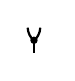
\begin{tikzpicture}[baseline=0.4ex, scale=0.4, line width=0.8pt]
		\path [use as bounding box] (0,0) rectangle (0.6,0.8);
		\draw (0.2,0) -- (0.2,0.4);
		\filldraw[black] (0.2,0.4) circle (0.08);
		\draw (0,0.8) .. controls (0,0.65) and (0.1,0.45) .. (0.2,0.4);
		\draw (0.4,0.8) .. controls (0.4,0.65) and (0.3,0.45) .. (0.2,0.4);
	\end{tikzpicture}%
}
\newcommand{\counit}{%
	\begin{tikzpicture}[baseline=0.4ex, scale=0.4, line width=0.8pt]
		\path [use as bounding box] (0,0) rectangle (0.4,0.8);
		\draw (0.2,0) -- (0.2,0.4);
		\filldraw[black] (0.2,0.4) circle (0.08);
	\end{tikzpicture}%
}

% camera-ready
\newcommand{\ifcameraready}[2]{\ifdefined\cameraready #2 \else #1 \fi}

\input{../../../sample.tikzstyles}
\input{../../../hypergraph.tikzstyles}
\input{../../../hypergraph.tikzdefs}


\def\BibTeX{{\rm B\kern-.05em{\sc i\kern-.025em b}\kern-.08em
    T\kern-.1667em\lower.7ex\hbox{E}\kern-.125emX}}
\begin{document}

\title{Equivalence Hypergraphs: DPO Rewriting for Monoidal E-Graphs}

% \author{\IEEEauthorblockN{1\textsuperscript{st} Given Name Surname}
% \IEEEauthorblockA{\textit{dept. name of organization (of Aff.)} \\
% \textit{name of organization (of Aff.)}\\
% City, Country \\
% email address or ORCID}
% \and
% }

\author{Anonymous}

\maketitle

\begin{abstract}
	The technique of equipping graphs with an equivalence relation, called equality saturation, has recently proved both powerful and practical in program optimisation, particularly for satisfiability modulo theory solvers. 
We give a categorical semantics to these structures, called e-graphs, in terms of Cartesian categories enriched over a category of semilattices.
We show how this semantics can be generalised to monoidal categories, which opens the door to new applications of e-graph techniques, from algebraic to monoidal theories.
Finally, we present a sound and complete combinatorial representation of morphisms in such a category,  based on a generalisation of hypergraphs which we call e-hypergraphs.
They have the usual advantage that many of their structural equations are absorbed into a general notion of isomorphism.    
\end{abstract}



% !TEX root = ../main.tex

\newcommand\mylet[2]{\textsf{let } #1 = #2 \textsf{ in }}


\cite{heijltjes_functional_2023}
\cite{barrett_functional_2023}
\cite{griggio_proceedings_2022}
\cite{flatt_small_2022}
\cite{ghica_operational_2021}
 % digital circuits
\cite{ghica_hierarchical_2023}
\cite{ghica_rewriting_2023} % traced comonoid
\cite{wilson_string_2023} % non-strict categories

\cite{zhang_relational_2022} % relational ematching 
\cite{alvarez-picallo_rewriting_2022} % hierarchical
\cite{alvarez-picallo_functorial_2021} % hierarchical 

\cite{bonchi_tape_nodate} % tape diagrams
\cite{baldan_categorical_2014} % signal flow
\cite{dpo}
\cite{maclane}
\cite{singher2023colored}



\section{Introduction}

Rewrite-driven program optimization consists of applying a sequence of semantics-preserving rewrites which may improve speed of execution, resource usage, \textit{etc}. Because early application of some rewrites can enable or block the subsequent application of others, the choice of application order hugely impacts the quality of the resulting optimization.  This long-standing issue is known as the \textit{phase-ordering problem}, with a \textit{phase} referring to a particular set of rewrites, for example,  those implementing constant propogation, loop unfolding, or unreachable code elimination. Typical approaches to this problem use heuristics to make an ad-hoc choice of ordering. 

A recently proposed,  alternative solution to this problem is \textit{equality saturation} 
\cite{10.1145/1594834.1480915}: instead of maintaining a \textit{single},  putatively optimized program which is rewritten \textit{destructively} at each step, we can maintain a \textit{set} of equivalent programs, where each rewrite step \textit{non-destructively} grows the set.  Upon reaching a fixed point (\textit{saturation}),  a \textit{globally} optimal program can then be extracted.% from the set,  which now represents all equivalent ways to express the program with respect to the given rewrites.  

The use of \textit{equality graphs (e-graphs)} \cite{EggPaper} -- a generalization of the typical directed acylcic graph (DAG) representation of terms to include equivalence classes -- to compactly represent the set of equivalent programs is what makes the technique tractable in practise, where the naive approach is clearly unfeasible. 

While equality saturation is a state-of-the-art optimization technique, the formal mathematical theory of e-graphs is perhaps underdeveloped. In this paper, we contribute a categorical understanding of e-graphs and their rewriting. Considering programs as represented by terms of an arbitrary algebraic theory, we demonstrate a correspondence between e-graphs and (string diagrams for) simple \textit{semilattice-enriched} Cartesian categories, where the semilattice \textit{join} allows us to consider formal sets of terms (string diagrams, morphisms). 

However, we do not develop the categorical perspective purely for its own sake: rephrasing the formalism of e-graphs in terms of algebraic theories and Cartesian categories suggests a natural generalization to monoidal theories. Therefore, our theoretical development leads to new potential domains of application, including optimziation of string diagrams representing digital \cite{ghica_compositional_2023} and quantum circuits
\cite{coecke_interacting_2011,ZX} and potentially to natural language \cite{wazni_quantum_2022,coecke_lambek_2013}.  We also suggest how our approach will allow future  generalization to include rewriting for the $\lambda$-calculus 
\cite{koehler2022sketchguided} % latest egraph. 

Towards implementation, we 
additionally provide a combinatorial representation of our enriched string diagrams in terms of (hierarchical)  hypergraphs.  We give a specification of hypergraph rewriting in this novel setting via a suitable extension of the double pushout (DPO) rewriting framework 
\cite{bonchi_string_2022-1,bonchi_string_2022-2,bonchi_string_2022},  thus also formalizing the rewriting theory of standard e-graphs. 

\subsection*{E-graphs}

\begin{figure}\label{fig:egraph-strings}
\[
    \tikzfig{categorical-semantics/egraph-strings}
\]
\caption{String diagrams for semilattice enriched symmetric monoidal categories.}
\end{figure}

\begin{figure}\label{fig:e-graph-example}
\[
    \scalebox{0.5}{
    \tikzfig{categorical-semantics/egraph-translation}
    }
\]
\caption{Example translation of e-graphs into string diagrams for semilattice enriched (traced) Cartesian categories.}
\end{figure}

\begin{figure}\label{fig:let-calculus}
\begin{align*}
    (a*2)/2 \\
    \mylet{y}{a*2} y/2 \\ 
    \mylet{y}{\{a*2,a<\!\!<1\}} y/2 \\
    \mylet{y}{\{a*2,a<\!\!<1\}} \{y/2, a*(2/2)\} \\
    \mylet{x}{\{2/2, 1\}} \mylet{y}{\{a*2, a <\!\!< 1\}} \{y/2, a*x\} \\
    \textsf{letrec } z = (\mylet{x}{\{2/2, 1\}} \mylet{y}{\{z*2, z <\!\!< 1\}} \{a, y/2, z*x\}) \textsf{ in } z
\end{align*}
\caption{Example term calculus corresponding to the string diagrams of Figure \ref{fig:e-graph-example}}
\end{figure}

E-graphs are a data structure which can efficiently represent many equivalent terms of an algebraic theory. They generalize the typical DAG representation of terms to include equivalence classes. 
A sequence of examples, taken from \cite{EggPaper}, are given in the first row of Figure \ref{fig:e-graph-example}. Here,  nodes (solid boxes) have children given by equivalence classes (dashed boxes) of nodes instead of just a single node.  Note, the equivalence classes relate nodes whose corresponding \textit{sub-trees} denote equivalent terms. 

Beginning with the e-graph (a), corresponding to the DAG representation of the term $(a*2)/2$, each subsequent e-graph (b)-(e) uses the given rewrite rule to add information: creating new nodes and edges, or merging equivalence classes. The final e-graph, (e), contains a cycle, and represents infinitely many terms: $a, a*1, (a*1)*1, $... 

\subsection*{Semantics via Semilattice Enriched Categories}

One can easily see the correspondence between (acyclic) e-graphs and morphisms of a suitably enriched Cartesian category by considering string diagrams 
\cite{noauthor_09083347_nodate,joyal_geometry_1991, mellies_functorial_2006}. In Figure \ref{fig:egraph-strings} we have extended the usual string diagrammatic notation for symmetric monoidal categories with an additional generator which has the  typing rule below, left.
The ability to take formal sums of morphisms is used to model the equivalence class structure of e-graphs.  
\[
\infer{\phi_1 + \ldots + \phi_n: A \to B}{\{\phi_i: A \to B\}_{i \in \{1,\ldots,n\}}}
\qquad
\infer{\Gamma \vdash \{t_1, \ldots, t_n\}: A}{\{\Gamma \vdash t_i: A\}_{i \in \{1, \ldots, n\}}}
\]
To aid understanding, in Figure \ref{fig:let-calculus} we give an example of a representation of the string diagrams in Figure \ref{fig:e-graph-example} using an informal let-calculus, which is standard except for its augmentation with the typing rule above, right, corresponding to semilattice enrichment. The new construct forms a set of terms and satisfies the following additional congruence: $K\{\{t_1, \ldots, t_n\}\} = \{K\{t_1\}, \ldots, K\{t_n\}\}$. 

String diagrams are read from bottom-to-top and we consider additional generators for the duplication and deletion transformations of a Cartesian category.  Note, further, that in the Cartesian case we can restrict to generators $c$ with a single output. 

The translation from e-graphs to our enriched string diagrams is illustrated informally below. 
Note how the typing constraints of the $+$ constructor are satisfied in the image of the translation by discarding in each component unnecessary inputs.
\[
    \tikzfig{categorical-semantics/egraph-translation-1}
\]

Examples of this translation are given in the second row of Figure \ref{fig:e-graph-example}. In particular, note that the translation of the \textit{cyclic} e-graph (e)
requires the use of a categorical \textit{trace}, generating a cycle. In this paper, we focus on \textit{acyclic} e-graphs and their corresponding catgeories; but the above example illustrates that the extension to the cyclic case appears routine.

Note how the natural level of generality for our string diagrams is not Cartesian, but monoidal: the generators of a Cartesian category are required in order to embed e-graphs, but are orthogonal to the addition of formal sums. Thus we generalize e-graphs from algebraic to monoidal theories. 

\subsection*{Combinatorial Representation of Enriched String Diagrams}

In order to \textit{implement} our generalized version of e-graphs, we will  perform rewriting not on algebraic terms, but on combinatorial representations of the corresponding string diagrams.  String diagrams can be considered equivalently as either topological objects (\textit{i.e.}, taken modulo "connectivity") or as a 2-dimensional syntax quotiented by the equations of an SMC. For example, we have the following equivalences between diagrams. 
%\[(f_1 \otimes f_2) ; (g_1 \otimes g_2) = (f_1 ; g_1) \otimes (f_2 ; g_2)\] 
\[
	\tikzfig{categorical-semantics/interchange}
\]

Unfortunately, this makes string diagrams relatively unamenable to efficient implementation as a data structure, due to the difficulty of calculating the quotient. 

Nevertheless, there is a body of work dealing with this issue by representing string diagrams as combinatorial objects -- namely, (appropriately generalized) hypergraphs 
\cite{bonchi_string_2022-1,bonchi_string_2022-2,bonchi_string_2022}.  Here, the generators $c_i$ become vertices which are connected via hyper-edges.  Thus the expected quotient becomes simply hypergraph isomorphism.  With appropriate restrictions on the form these hypergraphs can take, this approach can be used to \textit{characterize} the free symmetric monoidal category generated by some $c_i$. 

We are interested in not just the free SMC over a set of generators, but rather in \textit{symmetric monoidal theories} which involve considering extra equations between morphisms: for instance, the rewrite rules $(a)-(e)$ of Figure \ref{fig:e-graph-example}. These can be seen as equations between string diagrams, and thus between their hypergraph representations.  Because the generating equations can be applied in any context, we are lead to the notion of \textit{(hyper)graph rewriting}: given an equation $l=r$, we require some way to identify (a sub-hypergraph corresponding to) $l$ in any hypergraph $G$ and replace it with (a sub-hypergraph corresponding to) $r$.
The standard approach to this is known as\textit{double pushout (DPO) rewriting}. 

Our application requires a generalization of these concepts from hypergraphs to \textit{e-hypergraphs}, which we define as a hypergraph with two additional relations denoting the hierarchical structure introduced by "e-boxes" ( \textit{i.e.,} the generator for semilattice enrichment) and the separation of the components of each e-box.
Giving the appropriate definitions is slightly delicate matter, and constitutes the main body of the paper. 

\subsection*{Soundness and Completeness}
The main technical result of the paper is a proof soundness and completeness of the combinatorial representation for semilattice enriched SMCs, extending the results of \cite{bonchi_string_2022-2} for plain SMCs. While the structural equalities of SMCs are factored out in the representation,  important structural equalities arising from the enrichment (see the equations of Figure \ref{fig:string-equations}) are not, and should not be: they represent the un/sharing of subdiagrams with respect to the e-box structure,  which is precisely what allows for the compact representation of equivalence classes.  Instead, we consider DPO-rewrites implementing both the structural equalities for enrichment (which involve the e-box structure) and the equalities arising from the generating symmetric monoidal theory (which do not).  

Quotienting e-hypergraphs by the induced equivalence gives rise to a sound and complete model of semilattice enriched categories.  That is, we exhibit a translation functor $\llbracket-\rrbracket$ from the free semilattice enriched SMC over a symmetric monoidal theory to our (quotiented) category of e-hypergraphs such that 
morphisms $f = g$ if and only if there exists a sequence of DPO-rewrites (each induced by a structural equality or the theory) between their translations: $\llbracket f \rrbracket \rightsquigarrow \llbracket_{DPO} g \rrbracket$. 

\subsection*{E-matching and E-rewriting}

Having defined e-hypergraphs and shown them to correctly model rewriting string diagrams for SMCs, equipped with a notion of "equivalence class", we note that the naive implementation of DPO-rewriting is inefficient: to find a redex within an e-hypergraph involves finding a structurally equivalent e-hypergraph which contains the redex as a subgraph. In general, this involves unsharing the e-box structure before a redex becomes available. Thus, we define a notion of e-matching for e-hypergraphs: that is, to find redexes working modulo the e-structure. In particular, we wish to locate the smallest subgraph $G' \subset G$ "containing" the redex $L$. Given this, the analogue of e-rewriting $L \to R$ is simple to define, due to its non-destructive nature: we rewrite $G' \to G' + R$ in $G$. 

[Example diagrams]

\subsection*{Future Applications}

Example diagrams for circuits, trace (loop unrolling, PEGs), LC, ZX here.

\subsection{Related Work}
Q: Related work - at end? \\
% !TEX root = ../main.tex

\section{Combinatorial semantics}


\update{Below I will assume that we work with a simple PROP (not coloured)}

Before we begin we first fix some notation.
When $V$ is a set, we denote with $V^{*}$ a set of all finite sequences of the elements of $V$, i.e. $^*$ is a free monoid.
When $\phi : V \to V'$ is a function, we denote with $\phi^{*}$ an extension of $\phi$ to sequences, i.e. $\phi^{*} : V^* \to V'^{*}$ and it applies $\phi$ element-wise.
Similarly, in the case when $\psi \subset V \times V$ is a relation: we denote with $\psi^{*}: \subset V^* \times V^*$ the element-wise relation on ordered sequences.
We will denote with $A +_{f,g} B$ the pushout of $A \xleftarrow{f} C \xrightarrow{g} B$ and will use $i_j$ to denote the $j^{\text{th}}$ injection into a coproduct of the form $X_{j} \xrightarrow{i_{j}} X_{1} + \ldots X_{j} + \ldots X_{n}$ where $+$ denotes the coproduct.

There was a correspondence between hypergraphs and terms in $\textsf{PROP}(\Sigma)$ developed in~\cite{Frobenius, Frobenius2} which we will refer to throughout this section. We first recall the notion of a hypergraph from there.

\Aleksei{Actually, in~\cite{Frobenius} a hypergraph is defined as an object of the corresponding category and labelled hypergraphs are defined as a slice category. This is needed to show adhesiveness. As our category is not adhesive, I think we can follow a more straightforward definition of a tuple.}

\begin{definition}[Category $\catname{Hyp_{\Sigma}}$]


A hypergraph $\mathcal{G}_{\Sigma}$ over a monoidal signature $\Sigma$ is a tuple 
\[
(V_{\mathcal{G}},E_{\mathcal{G}},s,t,l)
\]
\label{def:hypergraph}

where $V_{\mathcal{G}}$ is the set of nodes, $E_{\mathcal{G}}$ is a set of edges, $s : E_{\mathcal{G}} \to V_{\mathcal{G}}^{*}$ is a source function that for each edge returns the ordered list of the edge's source nodes, $t : E_{\mathcal{G}} \to V_{\mathcal{G}}^{*}$ is a target function that for each edge returns the ordered list of the edge's target nodes, $l : E_{\mathcal{G}} \to \Sigma$ is a label function that labels each edge with a generator from monoidal signature $\Sigma$. The label function should satisfy the following conditions: $\forall e,\; \text{s.t.}\; l(e) : m \to n\;. \;|s(e)| = m$ and $\forall e,\; \text{s.t.}\; l(e) : m \to n \;. \;|t(e)| = n$

We will omit the subscripts when they are clear from the context.

A homomorphism $\phi: \mathcal{F} \to \mathcal{G}$ of hypergraphs $\mathcal{F},\mathcal{G}$ is a pair of functions $\phi_V : V_{\mathcal{F}} \to V_{\mathcal{G}}, \phi_E : E_{\mathcal{F}} \to E_{\mathcal{G}}$ such that

\begin{enumerate}
        \item $(s_{\mathcal{F}};\phi_V^*)(e) = (\phi_E;s_{\mathcal{G}})(e)$
    \item $(t_{\mathcal{F}};\phi_V^*)(e) = (\phi_E;t_{\mathcal{G}})(e)$
    \item $l_{\mathcal{F}}(e) = \phi_E;l_{\mathcal{G}}(e)$
\end{enumerate}


Hypergraphs over a monoidal signature $\Sigma$ together with hypergraph homomorphisms form a category $\catname{Hyp_{\Sigma}}$. 
\end{definition}

\begin{definition}[Definition 2.10~\cite{Frobenius}]
Let $\mathbb{C}$ be a category with all finite colimits. A cospan from $X$ to $Y$ is a pair of arrows $X \xrightarrow{} A \xleftarrow{} Y$  in $\mathbb{C}$.

Two cospans $X \xrightarrow{} A \xleftarrow{} Y$ and $X \xrightarrow{} B \xleftarrow{} Y$ are isomorphic if the following diagram commutes and $\alpha$ is iso.

\[
\begin{tikzcd}
                                               & A \arrow[dd, "\alpha"] &                                                \\
X \arrow[ru, bend left] \arrow[rd, bend right] &                        & Y \arrow[ld, bend left] \arrow[lu, bend right] \\
                                               & B                      &                                               
\end{tikzcd}
\]


For $X \in \mathbb{C}$ an $id$-cospan is $X \xrightarrow{id_X} X \xleftarrow{id_X} X$.
The composition of cospans $X \xrightarrow{} A \xleftarrow{f} Y$ and $Y \xrightarrow{g} B \xleftarrow{} Z$ is $X \xrightarrow{} A +_{f,g} B \xleftarrow{} Z$, constructed by taking a pushout of $f,g$.
This data is the category $\catname{Csp(\mathbb{C})}$: the objects are those of $\mathbb{C}$ and the arrows are isomorphism classes of cospans.
Finally, $\catname{Csp(\mathbb{C})}$ is a monoidal category: monoidal product is given by a coproduct (denoted with $+$) in $\mathbb{C}$ and the unit is given by the initial object of $\mathcal{C}$ as can be seen below.

% \[
% \adjustbox{scale=0.75,center}{
% https://q.uiver.app/#q=WzAsMTEsWzAsMCwiQSJdLFsxLDAsIlxcbWF0aGNhbHtHfSJdLFsyLDAsIkIiXSxbMywwLCJcXG90aW1lcyJdLFs0LDAsIkEnIl0sWzYsMCwiQiciXSxbNSwwLCJcXG1hdGhjYWx7Ryd9Il0sWzcsMCwiOj0iXSxbOCwwLCJBK0EnIl0sWzEwLDAsIlxcbWF0aGNhbHtHfStcXG1hdGhjYWx7Ryd9Il0sWzEyLDAsIkIrQiciXSxbMCwxLCJmIl0sWzIsMSwiZyIsMl0sWzQsNiwiZiciXSxbNSw2LCJnJyIsMl0sWzgsOSwiZitmJyJdLFsxMCw5LCJnK2cnIiwyXV0=
% \begin{tikzcd}
% 	A & {\mathcal{G}} & B & \otimes & {A'} & {\mathcal{G'}} & {B'} & {:=} & {A+A'} && {\mathcal{G}+\mathcal{G'}} && {B+B'}
% 	\arrow["f", from=1-1, to=1-2]
% 	\arrow["g"', from=1-3, to=1-2]
% 	\arrow["{f'}", from=1-5, to=1-6]
% 	\arrow["{g'}"', from=1-7, to=1-6]
% 	\arrow["{f+f'}", from=1-9, to=1-11]
% 	\arrow["{g+g'}"', from=1-13, to=1-11]
% \end{tikzcd}
\[
    A \xrightarrow{f} \mathcal{G} \xleftarrow{g} B \otimes A' \xrightarrow{f'} \mathcal{G'} \xleftarrow{g'} B' := A + A' \xrightarrow{f'} \mathcal{G} + \mathcal{G'} \xleftarrow{g'} B + B'
\]

Symmetry is inherited from $\mathcal{C}$ as the coproduct is commutative and is given below.

\[
n + m \xrightarrow{\sigma_{n,m}} m + n \xleftarrow{id + id} m + n
\]

This construction turns this data into a symmetric monoidal category~\cite{MonoidalCoproduct}.

\end{definition}


\begin{remark}
    
Taking isomorphism classes of cospans as morphisms turns $\catname{Csp(\mathbb{C})}$ into a proper category since pushouts are defined up to isomorphism and associative.
\end{remark}

When $\mathbb{C} = \catname{Hyp_{\Sigma}}$ we get a category of cospans of hypergraphs.
$\catname{Hyp_{\Sigma}}$ has all finite colimits and, in particular, coproduct is a disjoint union of two hypergraphs.
An empty hypergraph is the initial object in $Hyp_{\Sigma}$ and coproduct and pushout are defined on the underlying sets of nodes and edges.
Following~\cite{Frobenius2} morphisms in an SMC with a signature $\Sigma$ can be interpreted as particular cospans of hypergraphs. 

\begin{definition}[Category $\;\catname{Csp_{D}(Hyp_{\Sigma})}$]
\label{def:cspd}
Category $\catname{Csp_{D}(Hyp_{\Sigma})}$ is a \textit{full} sub-category of $\catname{Csp(Hyp_{\Sigma})}$ which has discrete hypergraphs as objects.
% \update{Assuming that $D$ is a functor from PROP to $\catname{Hyp_{\Sigma}}$, $\catname{Csp_{D}(Hyp_{\Sigma})}$ is also a PROP and hence an SMC (Theorem 3.6~\cite{Frobenius}).}
\end{definition}

In particular, this means that any morphism in $\catname{Csp_{D}(Hyp_{\Sigma})}$ is of the form $n \xrightarrow{} \mathcal{G} \xleftarrow{} m$,
where $n,\;m$ are discrete hypergraphs and $\mathcal{G}$ is an arbitrary hypergraph.
When string diagrams are interpreted as cospans of hypergraphs $n,m$ correspond to input and output interfaces of a string diagram respectively.
A pictorial representation of such a cospan is depicted below in Figure~\ref{fig:hypergraph_and_string_diagram}.
We use node labels to define mappings $n \to \mathcal{F}$ and $m \to \mathcal{F}$.

\begin{figure}
    \centering
    \begin{subfigure}{0.45\linewidth}
    \[
    \scalebox{0.6}{
	\tikzfig{combinatorial_semantics/mda-hypergraph-example}
   }
   \]
    \end{subfigure}
    \hfill
    \begin{subfigure}{0.45\linewidth}
        \[
        \raisebox{-0.6cm}{
        \scalebox{0.75}{
        \tikzfig{combinatorial_semantics/mda-hypergraph-example-string}
        }}
        \]
    \end{subfigure}
    \caption{Cospan of hypergraphs and corresponding string diagram}
    \label{fig:hypergraph_and_string_diagram}
\end{figure}

\begin{definition}[Degree of a node] 
The in-degree of a node $v$ in a hypergraph $\mathcal{G}$ is the number of hyperedges $e \in {E_\mathcal{G}}$ such that $v \in s(e)$  Similarly, the out-degree of $v$ is the number of edges $e \in E_\mathcal{G}$ such that $v \in t(e)$.
    
\end{definition}

\begin{definition}[Path]
    A path from $e_0$ to $e_{n-1}$ of length $n$ in a hypergraph $\mathcal{G}$ is an ordered sequence of edges $e_i \in E_{G}$ : $[e_0, e_1, \ldots, e_{n-1}]$ such that for all $i < n - 1$ some node $v \in t(e_i)$ is also in $s(e_{i+1})$.
\end{definition}

\begin{definition}[Acyclicity]
    A hypergraph is acyclic if it contains no paths of length $n > 0$ that start and end in the same edge $e$.
\end{definition}

\begin{definition}[Monogamy]
\label{def:monogamy_hyp}

We call a cospan $n \xrightarrow{f} \mathcal{G} \xleftarrow{g} m$ in $\catname{Csp_{D}(Hyp_{\Sigma})}$ monogamous directed acyclic if

\begin{enumerate}
    \item $\mathcal{G}$ is a directed acyclic hypergraph
    \item $f$ and $g$ are monos
    \item the in-degree and out-degree of every vertex of $\mathcal{G}$ is at most 1
    \item vertices of $\mathcal{G}$ with in-degree 0 are precisely the image of $f$
    \item vertices of $\mathcal{G}$ with out-degree 0 are precisely the image of $g$
\end{enumerate}

\end{definition}

When we narrow our attention to cospans (morphisms) of $\catname{Csp_{D}(Hyp_{\Sigma})}$ which are monogamous we get the category of monogamous directed acyclic (mda-) cospans of hypegraphs $\MdaCospans$.

\begin{definition}[Category $\MdaCospans$]
    We define $\MdaCospans$ as a subcategory of $\catname{Csp_{D}(Hyp_{\Sigma})}$.
\end{definition}

Vertical and horizontal compositions of mda-cospans are mda-cospans, identities and symmetries are mda-cospans, tensor unit is discrete, and hence this is a proper symmetric monoidal category~\cite{Frobenius2}.


\begin{theorem}[Corollary 26~\cite{Frobenius2}]
    $\textsf{PROP}(\Sigma) \cong \MdaCospans$
\end{theorem}
This theorem essentially states a correspondence between morphisms in SMC (string diagrams) and mda-cospans of hypergraphs.

\begin{remark}[Pushout in $\catname{Hyp_{\Sigma}}$]
    Consider a diagram below
    % https://tikzcd.yichuanshen.de/#N4Igdg9gJgpgziAXAbVABwnAlgFyxMJZABgBpiBdUkANwEMAbAVxiRAC0QBfU9TXfIRQBGclVqMWbABrdeIDNjwEiZYePrNWiEAE05fJYKKj11TVJ0AdK3ABmAJzoBjYNIDUursBvYAtgAEAEpcBgr8ykLIAEyk0RqS2iAAitziMFAA5vBEoI4QfkhkIDgQSKISWmx2YfmFiMWlSLGVliCZINQMdABGMAwAChHGOg5YmQAWOLUOBeXUTYgAzOaJbL6OLsBYAPrC3r5YgSEzc4gtiyutSRtOrrvRB7ZHwaE8ebP1F2WIACzUfTAUCQAFolsULEkAFY7aKdEDdPqDYYqUbjKaneoVRb-ECA4HLCFrHQw4SYpBXHGrKo6JhpLhAA

\[
    \adjustbox{scale=1}{
        \begin{tikzcd}
        Z \arrow[r, "f"] \arrow[d, "g"']                                   & X \arrow[d, "\sfrac{i_1}{\sim R}"] \arrow[rdd, "j_1", bend left] &   \\
        Y \arrow[r, "\sfrac{i_2}{\sim R}"] \arrow[rrd, "j_2"', bend right] & \sfrac{X+Y}{\sim R} \arrow[rd, "u"]                              &   \\
                                                                        &                                                                  & Q
        \end{tikzcd}
    }
\]

Pushout of two hypergraphs $X = \{V_{X}, E_{X}, s_{X}, t_{X}\}$ and $Y = \{V_{Y}, E_{Y}, s_{Y}, t_{Y}\}$ (we will omit labelling functions here since they are irrelevant) along $Z$ is computed in two steps.
First, a coproduct of $X$ and $Y$ is taken which is 
\[
    X + Y = \{V_{X} + V_{Y}, E_{X} + E_{Y}, s_{X + Y}, t_{X+Y}\}
\]
where $s_{X+Y} : E_{X} + E_{Y} \to (V_{X} + V_{Y})^{*}$ which can be defined as a copairing $\langle s'_{X}, s'_{Y} \rangle : E_{X} + E_{Y} \to (V_{X} + V_{Y})^{*}$ and $s'_{X} : E_{X} \to (V_{X} + V_{Y})^{*}$, $s'_{Y} : E_{Y} \to (V_{X} + V_{Y})^{*}$ defined as $s'_{X} = s_{X};i_{1,V}^{*}$ and $s'_{Y} = s_{Y};i_{2,V}^{*}$ where $i_1,i_2$ are corresponding coproduct injections, similarly for $t_{X+Y}$.
Recall that each arrow in $\catname{Hyp_{\Sigma}}$ is a pair of arrows for edges and nodes and we will further use subscripts $V$ and $E$ when referring to these functions.
Then, consider relations 
\[
    S_{V} = \{(x_i,y_j) \in (V_{X} + V_{Y}) \times (V_{X} + V_{Y})\; | \; \exists z \in V_{Z} \; . \; x_i = f_{V};i_{1,V}(z) \text{ and } y_j = g_{V};i_{2,V}(z) \text{where $x_i \in V_{X}$ and $y_j \in V_{Y}$ }\}
\]
\[
    S_{E} = \{(x_i,y_j) \in (E_{X} + E_{Y}) \times (E_{X} + E_{Y})\; | \; \exists z \in E_{Z} \; . \; x_i = f_{E};i_{1,E}(z) \text{ and } y_j = g_{E};i_{2,E}(z) \text{where $x_i \in E_{X}$ and $y_j \in E_{Y}$ }\}
\]
and let relations $R_{V}$ and $R_{E}$ be their reflexive symmetric and transitive closures respectively.

\begin{lemma}
    $x R y$ if and only if either $x = y$ or there exists a sequence $(a_1,\ldots,a_{n-1},{a_n})$ such that $x = a_1$ and $y = a_{n}$ such that $a_k S a_{k+1}$ or $a_{k + 1} S a_{k}$ for $k < n$.
\end{lemma}

A quotient of $X+Y$ by these relation is 
\[
    \sfrac{X+Y}{\sim (R_{V},R_{E})} = \{\sfrac{V_{X} + V_{Y}}{\sim R_{V}}, \sfrac{E_{X} + E_{Y}}{\sim R_{E}}, \sfrac{s_{X+Y}}{\sim (R_{V},R_{E})}, \sfrac{t_{X+Y}}{\sim (R_{V},R_{E})}\}
\]
We will then refer to $\sim (R_{V},R_{E})$ just as $\sim$, i.e. writing $\sfrac{V_{X} + V_{Y}}{\sim}$ and the exact relation will be clear from the context.
We have 
\[
    \sfrac{s_{X+Y}}{\sim} : \sfrac{E_{X} + E_{Y}}{\sim} \to (\sfrac{V_{X} + V_{Y}}{\sim})^{*}
\]
In particular, there is an obvious surjective function $[-]_{V} : (V_{X} + V_{Y}) \to (\sfrac{V_{X} + V_{Y}}{\sim})$ that maps elements to their equivalence classes and $[-]_{V}^{*}$ is its extension to sequences. 
Let $s_2 : E_{X} + E_{Y} \to (\sfrac{V_{X} + V_{Y}}{\sim})^{*} = s_{X+Y};[-]^{*}$ and then $\sfrac{s_{X+Y}}{\sim}([e]) = s_{X+Y};[-]^{*}(e) = [s_{X+Y}(e)]^{*}$.
There is also $[-] : E_{X} + E_{Y} \to \sfrac{E_{X} + E_{Y}}{\sim}$ and we will omit subscripts as the correct type will be clear from the argument.
We will also use subscripts when it is important to tell if an element of $E_{X} + E_{Y}$ has in image in either $E_{X}$ or $E_{Y}$ by writing $e_{x}$ or $e_{y}$.
We need to check that if $t_1 \sim t_2$ then $\sfrac{s_{X+Y}}{\sim}([t_1]) = \sfrac{s_{X+Y}}{\sim}([t_2])$. 
There are three options
\begin{enumerate}
    \item $t_1 = e_{y}^{1}$ and $t_2 = e_{y}^{2}$
    \item $t_1 = e_{x}^{1}$ and $t_2 = e_{x}^{2}$
    \item $t_1 = e_{x}$ and $t_2 = e_{y}$ 
\end{enumerate}
We will prove the last point (all the others are analogous).
\begin{proof}
    According to the lemma above $e_{x} \sim e_{y}$ gives us two options.
    \begin{enumerate}
        \item Either $e_{x} = e_{y}$
        \item or there is a sequence $w = (a_1, \ldots, a_{n})$ such that $a_1 = e_{x}$ and $a_{n} = e_{y}$.
    \end{enumerate}
    In the first case the equality holds on the nose.
    We then prove the second case by induction on the length of $w$.
    \begin{itemize}
        \item In the case $|w| = 2$, $e_{x} S e_{y}$ (or $e_{y} S e_{x}$) which means that there exists $z$ in $E_{Z}$ such that $f_{E};i_{1,E}(z) = e_{x}$ and $g_{E};i_{2,E}(z) = e_{y}$.
              Recall that because $f$ and $g$ are homomorphisms, the following equalities hold
              \[
                s_{Z};f_{V}^{*};i_{1,V}^{*}(z) = f_{E};i_{1,E};s_{X+Y}(z) = s_{X+Y}(e_{x})
              \]
              \[
                s_{Z};g_{V}^{*};i_{2,V}^{*}(z) = g_{E};i_{2,E};s_{X+Y}(z) = s_{X+Y}(e_{y})
              \]
              Then,
              \[
                \sfrac{s_{X+Y}}{\sim}([e_{x}]) = [s_{X+Y}(e_{x})]^{*} = [s_{Z};f_{V}^{*};i_{1,V}^{*}(z)]^{*}
              \]
              and
              \[
                \sfrac{s_{X+Y}}{\sim}([e_{y}]) = [s_{X+Y}(e_{y})]^{*} = [s_{Z};g_{V}^{*};i_{2,V}^{*}(z)]^{*}
              \]
              Then, by noting that $f_{V};i_{1,V}(z) = g_{V};i_{2,V}(z)$ for all $z$ in $V_{Z}$ (because $\sfrac{V_{X} + V_{Y}}{\sim}$ is so defined) we have $[s_{X+Y};(e_{x})]^{*} = [s_{X+Y}(e_{y})]^{*}$.
        \item Suppose if $e_{x} S e_{y}$ by a chain of length $n$ or less then $[s_{X+Y}(e_{x})]^{*} = [s_{X+Y}(e_{y})]^{*}$.
        \item Now suppose $e_{x} S e_{y}$ by a chain $w = (a_1, \ldots, a_{n+1})$ and a subchain $(a_1, \ldots, a_{n})$ satisfies the inductive hypothesis and hence $s_{X+Y};s_{1}^{*}(e_{x}) = s_{X+Y};s_{1}^{*}(a_{n})$.
              Note that $S_{E}, S_{V}$ relate only elements with the pre-image in $E_{X}$ (respectively, $V_{X}$) with elements with the pre-image in $E_{Y}$ (respectively, $V_{Y}$). 
              Elements with the pre-image in the same set are not related.
              Then we have $a_n S a_{n+1} = e_{y}$ and need to show that $[s_{X+Y}(a_{n+1})]^{*} = [s_{X+Y}(e_{y})]^{*}$.
              This follows by exactly the same argument as the base case as $a_{n+1}$ is necessarily in $E_{X}$.
              And we finally have $[s_{X+Y}(e_{x})]^{*} = [s_{X+Y}(a_{n+1})]^{*} = [s_{X+Y}(e_{y})]^{*}$.
    \end{itemize}
\end{proof}

Next 
\[
    \sfrac{i_{1,V}}{\sim} : V_{X} \to \sfrac{V_{X} + V_{Y}}{\sim} = [i_{1,V}]
\]
and
\[
\sfrac{i_{1,E}}{\sim} : E_{X} \to \sfrac{E_{X} + E_{Y}}{\sim} = [i_{1,E}]
\]
similarly for $\sfrac{i_{2,E}}{\sim}$ and $\sfrac{i_{2,V}}{\sim}$
We need to show
\begin{enumerate}
    \item $s_{X};(\sfrac{i_{1,V}}{\sim})^{*}(e) = \sfrac{i_{1,E}}{\sim};\sfrac{s_{X+Y}}{\sim}(e)$
    \item $t_{X};(\sfrac{i_{1,V}}{\sim})^{*}(e) = \sfrac{i_{1,E}}{\sim};\sfrac{t_{X+Y}}{\sim}(e)$
\end{enumerate}
and likewise for $i_{2}$.
Let's check the first one for which we first need to check that $([-]_{E},[-]_{V})$ is a homomorphisms, i.e.
\[
[s_{X+Y}(e)]^{*} = \sfrac{s_{X+Y}}{\sim}([e]) = [s_{X+Y}(e)]^{*}
\]
hence, $(\sfrac{i_{1,V}}{\sim}, \sfrac{i_{1,E}}{\sim})$ is a homomorphism because $(i_{1,V},i_{1,E})$ and $([-]_{E},[-]_{V})$ are.

% Note that if $s : e_1 \mapsto \{v_1,v_2\}$ and $s : e_2 \mapsto \{v_3,v_4\}$  and $e_1 \sim e_2$ then $\sfrac{s}{\sim R} : [e_1,e_2] \to \{[v_1,v_3],[v_2,v_4]\}$ because $f$ and $g$ are homomorphisms.
% Then, $\sfrac{i_1}{\sim R}$ maps $y \in Y$ to its equivalence class and likewise for $\sfrac{i_2}{\sim R}$.
% we will denote the equivalence classes in $\sfrac{X + Y}{\sim R}$ as $[x]$ and $[y]$ depending on their pre-image being either in $X$ or $Y$.
% Before we procced, we need to show that $\sfrac{i_1}{\sim R}$ and $\sfrac{i_2}{\sim R}$ are homomorphisms.
% Let $e_{x}$ be an edge in $X$ and $v_x$ is its source. We need to check that $\sfrac{i_1}{\sim R}(v_x) = (\sfrac{i_1}{\sim R};\sfrac{s_{X}}{\sim R})(e_x)$.
% $\sfrac{i_1}{\sim R}(v_x) = [v_x]$ and $(\sfrac{i_1}{\sim R};\sfrac{s_{X}}{\sim R})(e_x) = \sfrac{s_{X}}{\sim R}([e_x]) = [v_x]$ and hence $\sfrac{i_1}{\sim R}$ is a homomorphism, simialrly $\sfrac{i_2}{\sim R}$ is.
Now, the square obviously commutes.
To show that $\sfrac{X + Y}{\sim}$ is a pushout we need to argue that for each $Q$ and morphisms $j_1 = (j_{1,V}, j_{1,E})$ and $j_2 = (j_{2,V}, j_{2,E})$ such that the above square commutes there is a unique $u = (u_{V}, u_{E})$ such that $j_1 = \sfrac{i_{1}}{\sim} ; u$ and $j_2 = \sfrac{i_2}{\sim} ; u$.
We will define such $u$ as $u_{E}([i_{1,E}(e_{x})]) = j_{1,E}(e_{x})$ and $u_{E}([i_{2,E}(e_{y})]) = j_{2,E}(e_y)$ (similarly for $u_{V}$) and claim that it is a well-defined function by showing that if $t_1 \sim t_2$ then $u_{E}(t_1) = u_{E}(t_2)$.
There are three options analogoues to the proof above, so we will show the base case for $t_1 = i_{1,E}(e_{x})$ and $t_2 = i_{2,E}(e_{y})$.
$t_1 \sim t_2$ implies that there exists at least one $z$ in $E_{Z}$ such that $i_{1,E}(e_{x}) = f_{E};i_{1,E}(z)$ (or $e_{x} = f_{E}(z)$) and $[i_{1,E}(e_{x})] = \sfrac{i_{1,V}}{\sim}(e_x)$, and $e_y = g_{E}(z)$ $[in_{2,E}(e_{y})] = \sfrac{i_{2,V}}{\sim}(e_y)$.
By applying $j_{1,E}$ to the first we get $j_{1,E}(f_{E}(z)) = j_{1,E}(e_x)$ and similarly for $j_{2,E}$: $j_{2,E}(g_{E}(z)) = j_{2,E}(e_y)$ and $j_{1,E}(e_{x}) = j_{2,E}(e_{y})$ by commutativity.
Hence, $u_{E}([in_{1,E}(e_x)]) = u_{E}([in_{2,E}(e_y)])$.
% \update{Above $e_x$ and $e_y$ are different from $e_x$ and $e_y$ from the first proof, i.e. they are in $E_{X}$ and $E_{Y}$. This is probablty not good.}

Next, $u$ is a homomorphism because $j_1$ and $j_2$ are.
Finally, $u$ is unique.
Assume, that there exists $w : \sfrac{X+Y}{\sim R} \to Q$ for the same $j_1$ and $j_2$.
In order for them to commute $w_{E}([i_{1,E}(x)]) = j_1(x)$ and $w([in_{2,E}(y)]) = j_2(y)$ (similarly for $w_{V}$) which is the same as $u_{E}$.
That is, $j_1$ and $j_2$ determine $u$ uniquely.

\end{remark}

Now we are ready to define e-hypergraphs which are a combinatorial representation of enriched PROPs.

\begin{definition}[E-hypergraph]

    An e-hypergraph $\mathcal{G}$ over a monoidal signature $\Sigma$ is a tuple \[(V_{\mathcal{G}},E_{\mathcal{G}},s,t,l,<_c,\#)\] where $(V_{\mathcal{G}},E_{\mathcal{G}},s,t)$ are the same as in~\ref{def:hypergraph}.
    The labelling $l$ is modified to include an extra value $\bot \;$ $l :E_{\mathcal{G}} \to \Sigma + 1$. 
    % With an abuse of notation, we will confuse $\mathcal{G}$ with $V_{\mathcal{G}} \cup E_{\mathcal{G}}$, when treating it as a set.    
    $<_c \subset (V_\mathcal{G} + E_\mathcal{G}) \times (V_\mathcal{G} + E_\mathcal{G})$ is a child relation imposing a strict partial order on $(V_\mathcal{G} + E_\mathcal{G})$.
    We require that for a given $x \in (V_\mathcal{G} + E_\mathcal{G})$ a set of all predecessors of $x\;$ $[x) = \{x' \in E_\mathcal{G} \;||\; x' <_c x\; \}$ is finite and consists of edges $e \in E_{\mathcal{G}}$ such that $l(e) = \bot$ only.
    Next, each $x$ has at most one immediate predecessor.
    We will denote the fact that $e$ is an immediate predecessor of $v$ as $e <_c^{\mu} v$.
    Similarly, a set of all successors is $(x] = \{x' \in (V_\mathcal{G} + E_\mathcal{G}) \; ||\; x <_{c} x'\}$ where $x'$ can be a node or an edge. 
    % An edge $e \in E_{\mathcal{G}}$ is unlabelled, i.e. $l(e) = \bot$ iff $(e] \not = \varnothing$.
    Finally, we require that $<_c^{\mu}$ respects connectivity, i.e. if $v \in s(e)$ then $e' <_c^{\mu} e$ iff $e' <_c^{\mu} v$.

    Then, consider a relation $\consistency^{\mu} \subseteq (V_{\mathcal{G}} + E_{\mathcal{G}}) \times (V_{\mathcal{G}} + E_{\mathcal{G}})$ which we will call a \textit{consistency} relation and which has the following properties.
    \begin{enumerate}
        \label{def:consistency_properties}
        \item The relation is an equivalence relation
        \item If $v \in s(e)$ then $v \consistency^{\mu} e$
        \item If $v \in t(e)$ then $v \consistency^{\mu} e$
        \item The relation is defined only for edges $e$ and nodes $v$ such that $[v) = [e) \not = \varnothing$
    \end{enumerate}
    
%     $\langle (V_\mathcal{G} + E_\mathcal{G}), <_c, \# \rangle$ is an event-structure where $\# \subset (V_\mathcal{G} + E_\mathcal{G}) \times (V_\mathcal{G} + E_\mathcal{G})$ is an irreflexive symmetric relation called \textit{conflict} relation which satisfies the following
%     \begin{enumerate}
%         \label{def:e-hypergraph-req}
%         \item 
%         \[
%     \forall x_1, x_2, x_3 \in (V_\mathcal{G} + E_\mathcal{G}) \text{, if } x_1 <_c x_2 \text{ and } x_1 \# x_3 \text{ then } x_2 \# x_3
%     \] 
%     if $x_1 <_c x_2$ we say that conflict $x_2 \# x_3$ is inherited from the conflict $x_1 \# x_3$. If the conflict is not inherited we say it is \textit{immediate} and denote it with $\#_{\mu}$
%     \item $<_c$ and $\#$ are mutually exclusive
%     \item $\#$ is defined \textit{only} for $x \in (V_\mathcal{G} + E_\mathcal{G})$ such that $[x) \not \eq \varnothing$
%     \item $\#$ should respect connectivity
%     \item \update{Complement of $\hashtag_{\mu}$ should be transitive}
%     \item for all distinct $x_1, x_2, x_3 \in (V_\mathcal{G} + E_\mathcal{G})$ $x_1 \#_{\mu} x_2$ and $x_2 \#_{\mu} x_3$ implies $x_1 \#_{\mu} x_3$
%     \item for all $x, x' \in (V_\mathcal{G} + E_\mathcal{G})$ $x \#_{\mu} x'$ implies $[x) = [x')$
%         \end{enumerate}

% The last two requirements are known as \textit{confusion freeness}~\cite{ConfusionFreeEvents}.
\end{definition}

% Intuitively, the child and conflict relation together make it possible to model e-classes in our e-hypergraphs: an unlabelled edge $e$ represents an e-class where the children of $e$ that are in immediate conflict correspond to nodes and edges in different e-class instances.
% Condition (5) states that the following situation is not possible: $x_1 \# x_3$ and $x_1 \bar{\#} x_2$ and $x_2 \bar{\#} x_3$.
% Transitivity of $\bar{\#}$ requires that in this case $x_1 \bar{\#} x_3$.

% \begin{lemma}[Complement of $\#$ is equivalence relation]
% \begin{proof}
% As $\#$ is irreflexive then its complement $\bar{\#}$ is reflexive because $\forall x \; . \; (x,x) \not \in \#$. Because $\#$ is symmetric so is $\bar{\#}$, otherwise if $(x_1, x_2) \in \bar{\#}$ and $(x_2,x_1) \not \in \bar{\#}$ then $(x_2,x_1) \in {\#}$ which is symmetric and hence $(x_1,x_2)$ should be in ${\#}$.
% Finally, the complement is transitive because of (5).

% \end{proof}
% \end{lemma}


\begin{remark}
    We will further call edges $e$ such that $l(e) = \bot$ \textit{hierarchical}.
    We will also refer to edges $e$ and nodes $v$ such that $[e) = \varnothing$ and $[v) = \varnothing$ as top-level.
\end{remark}

\begin{remark}
    Because $\consistency^{\mu}$ respects connectivity and is reflexive, symmetric and transitive, it is essentially a relation between connected components that have the same predecessor.
    This notion will be helpful in the following example.
\end{remark}
% We associate an e-class with a hierarchical edge, i.e. an edge with children. 
% The parent functions satisfy some conditions. First, an edge and any of its source and target vertices must have the same parent: $p_V (v) = p_E(e) = p_V (v')$ for all $v \in s(e)$ and $v' \in t(e)$, respectively.
% Second, the parent relation must be acyclic.
% More precisely, we assume for all $e \in E$ there is some $k \geq 1$ such that $(p_E,\bot)k(e) = \bot$ where $\bot$ is the element of $1$ and $p_{E,\bot} :E+1 \to E+1$ is the extension of $p_E$ adding $p_{E,\bot}(\bot)=\bot$.


% $\#_{V}$ and $\#_{E}$ are conflict relations that tell whether nodes and edges belong to different instances within an e-class: if the elements are in conflict, they belong to different instances. \update{E-classes are represented by edges $e : l_E(e) = \bot$. Hence, the conflict relation $\#_{V}$ between $v_1$ and $v_2$ is defined only when $p_V(e_1) \not \eq \bot$ and $p_V(e_2) \not \eq \bot$. Likewise the conflict relation $\#_{E}$ between $e_1$ and $e_2$ is defined only when $p_{E}(e_1) \not \eq \bot$ and $p_{E}(e_2) \not \eq \bot$}



% The relation should respect connectivity, that is, if $e_1 \#_E e_2$ then $s(e_1) \#_V^* s(e_2)$ and $t(e_1) \#_V^* t(e_2)$, where $\#_V^*$ is element-wise relation. 
% % This guarantees that related nodes and edges are contained within the same e-class.
% \update{
% We also require that if $v_1 \#_{V} v_2$ then $\forall e_1,e_2 : v_1 \in s(e_1)$ and $v_2 \in s(e_2)\; e_1 \#_{E} e_2$  and the same for the case when $v_i \in t(e_1),\;v_j \in t(e_2)$. Finally, the relation should be \textit{hereditary}: if $e_1 \#_E e_2 \text{ and } \forall n,m,k,q > 0, \; v_1,v_2 \in V_{\mathcal{G}} \text{ and } e_1', e_2' \in E_{\mathcal{G}} \text{ s.t. } p^n(v_1) = e_1, \; p^m(v_2) = e_2, \; p^k(e_1') = e_1, \; p^q(e_2') = e_2\; . \;
%  v_1 \#_V v_2 \text{ and } e_1' \#_E e_2'$. Where $p^n(v),\; n > 0$ is $n^{th}$ parent of $v$} The relation is also irreflexive and symmetric.

\begin{example}
    
A few examples of e-hypergraphs (and their corresponding graphical interpretation) can be seen in Figure~\ref{fig:e-hypergraph-example}.
In example~\ref{fig:example_a} the relations $<_{c}$ and $\consistency^{\mu}$ are the following
\[
    <_{c} = \{(v_3,e_1), (e_2, e_1), (v_4, e_1) \}
\] and 
\begin{align*}
    \consistency^{\mu} = \{ (v_1,e_1),
                            (v_2, e_1), 
                            (v_3,e_2), (v_4,e_2)\}^{c}
\end{align*}
where $c$ denotes the reflexive, syymetric and transitive closure.
In other words, $e_1$ is the predecessor of the connected component that contains edge $e_2$ and this connected component is consistent with itself only.
The connected component that contains $e_1$ is also consistent with itself only.

In the next example~\ref{fig:example_b} $e_1$ is the predecessor of two connected components but these components are consistent only with themselves.
We denote this fact by using a vertical line. 
Practically, hierarchical edges such as $e_1$ represent e-classes and connected components which are pairwise not consistent belong to different instances of the same e-class.

In the last example~\ref{fig:example_c} two connected components that contain $e_2$ and $e_3$ respectively are consistent with themselves and with each other.
\end{example}

\begin{figure}[t]
    \begin{subfigure}{0.3\linewidth}
        \[
            \scalebox{0.6}{
                \tikzfig{combinatorial_semantics/e-hypergraph-example-1}
            }
            \]
        \caption{}
        \label{fig:example_a}
    \end{subfigure}
    \hfill
    \begin{subfigure}{0.3\linewidth}
        \[
          \scalebox{0.6}{
            \tikzfig{combinatorial_semantics/e-hypergraph-example-2}
          }  
        \]
        \caption{}
        \label{fig:example_b}
    \end{subfigure}
    \hfill
    \begin{subfigure}{0.3\linewidth}
        \[
          \scalebox{0.6}{
            \tikzfig{combinatorial_semantics/e-hypergraph-example-3}
          }  
        \]
        \caption{}
        \label{fig:example_c}
    \end{subfigure}
    \caption{E-hypergraph examples}
    \label{fig:e-hypergraph-example}
\end{figure}

\begin{example}
An example of an e-hypergraph can be found in Figure~\ref{fig:e-cospan}.
The e-hypergraph is depicted in the area shaded grey.
Edges $g$ and $h$ are in conflict (as well as their incoming and outcoming nodes) and they share the same predecessor --- the edge shaded with lighter colour. 
Vertical line delimits the edges and nodes which are in conflict. 
Intuitively, such lines delimit e-class instances.
\end{example}

\begin{definition}[Convex subgraph]
  We call a subgraph $\mathcal{H}$ of an e-hypergraph $\mathcal{G}$ convex if for all $v_i, v_j \in V_{\mathcal{H}}$ all $v_k \in path(v_i, v_j)$ are also in $\mathcal{H}$.
\end{definition}


\begin{definition}[Down-closed subgraph]
    We call a subgraph $\mathcal{H}$ of an e-hypergraph $\mathcal{G}$ down-closed if for all $e \in E_{\mathcal{H}}$ all elements of $(e]$ are also in $\mathcal{H}$.
\end{definition}

 % \begin{remark}
 %    We will use $p_{E}^n(e)$ as a syntactic sugar for $p_{E,\bot} ; p_{E,\bot} \ldots p_{E,\bot}(e)$ to denote the n$^{th}$ parent of an edge $e$. Similarly
 %     we will use $p_{V}^n(v)$ as a syntactic sugar for $p_{E}^{n-1};p_{V}(v)$ to denote the n$^{th}$ parent of a node $v$.
 % \end{remark}

\begin{remark}
    Both relations can be considered as functions defined on $V_{\mathcal{F}} + E_{\mathcal{F}}$, i.e. on the coproduct of nodes and edges.
    To make things well-typed, we will use corresponding coproduct injections $i_{V_{\mathcal{F}}} \to V_{\mathcal{F}} + E_{\mathcal{F}}$ and $i_{E_{\mathcal{F}}} \to V_{\mathcal{F}} + E_{\mathcal{F}}$ when passing either node or edge into these functions.
    For example, an immediate successor of a node $x$ can be written functionally as $<_{c,\mathcal{F}}^{\mu}(i_{V_{\mathcal{F}}}(x))$.
\end{remark}

\begin{definition}{E-hypergraphs homomorphism}
\label{def:e-homo}    
A homomorphism $\phi: \mathcal{F} \to \mathcal{G}$ of e-hypergraphs $\mathcal{F},\mathcal{G}$ is a pair of functions $\phi_V : V_{\mathcal{F}} \to V_{\mathcal{G}}, \phi_E : E_{\mathcal{F}} \to E_{\mathcal{G}}$ such that

\begin{enumerate}
    \item $\phi$ is hypergraph homomorphism
    
    \item \[
        \phi_{E}(<_{c,\mathcal{F}}^{\mu}(i_{V_{\mathcal{F}}}(x))) = <_{c,\mathcal{G}}^{\mu}(\phi_{V};i_{V_{\mathcal{G}}}(x))
        \] when $x$ is a node,
        and
        \[
        \phi_{E}(<_{c,\mathcal{F}}^{\mu}(i_{E_{\mathcal{F}}}(x))) = <_{c,\mathcal{G}}^{\mu}(\phi_{E};i_{E_{\mathcal{G}}}(x))  
        \] when $x$ is an edge.
        We do not require such an equation when $[x) = \varnothing$.

    % \item
    % $x_1 \#_{\mathcal{F}} x_2$ iff $\phi(x_1) \#_{\mathcal{G}} \phi(x_2)$, where $x_1, x_2 \in \mathcal{F}$
  
        \item
    if $x_1 \consistency_{\mathcal{F}}^{\mu} x_2$ then $\phi(x_1) \consistency_{\mathcal{G}}^{\mu} \phi(x_2)$, where $x_1, x_2 \in \mathcal{F}$.
    Or, written functionally, when $x \in E_{\mathcal{F}}$
    \[
        \langle \phi_{V};i_{V_{\mathcal{G}}}, \phi_{E};i_{E_{\mathcal{G}}} \rangle^{*}(\consistency_{\mathcal{F}}^{\mu}(i_{E_{\mathcal{F}}}(x)))
        \subseteq
        \consistency_{\mathcal{G}}^{\mu}(\phi_{E};i_{E_{\mathcal{G}}}(x))
    \]
    , where $\phi_{V};i_{V_{\mathcal{G}}} : V_{\mathcal{F}} \to V_{\mathcal{G}} + E_{\mathcal{G}}$, and similarly for $\phi_{E};i_{E_\mathcal{G}}$ so that $\langle \phi_{V};i_{V_{\mathcal{G}}}, \phi_{E};i_{E_{\mathcal{G}}} \rangle : V_{\mathcal{F}} + E_{\mathcal{F}} \to  V_{\mathcal{G}} + E_{\mathcal{G}}$.
    And, when $x \in V_{\mathcal{F}}$
    \[
        \langle \phi_{V};i_{V_{\mathcal{G}}}, \phi_{E};i_{E_{\mathcal{G}}} \rangle^{*}(\consistency_{\mathcal{F}}^{\mu}(i_{V_{\mathcal{F}}}(x)))
        \subseteq
        \consistency_{\mathcal{G}}^{\mu}(\phi_{V};i_{V_{\mathcal{G}}}(x))
    \]
    % Or, on per-component basis, if $i_{E_{\mathcal{F}}}(x_1) \in \hashtag_{\mathcal{F}}(i_{E_{\mathcal{F}}}(x_2))$ then $i_{E_{\mathcal{G}}}(\phi_{E}(x_1)) \in \hashtag_{\mathcal{G}}(i_{E_{\mathcal{G}}}(\phi_{E}(x_2)))$ and similarly for other types of $x_1,x_2$.
\end{enumerate}

% \update{Let's denote the fact of $x_1$ being the immediate predecessor of $x_2$ by $x_1 <_{\mu} x_2$.
%  Also, note that preserving the immediate predecessor implies preserving order.
% Homomorphism definition seems to be fine: by not requiring the \textit{only if} direction in bullet 2 we basically allow either of two things 

% \begin{itemize}
%     \item $\phi(x_1) <_{\mu} \phi(x_2)$ and $x_1 <_{\mu} x_2$
%     \item $\phi(x_1) <_{\mu} \phi(x_2)$ and $x_1$ is unrelated to $x_2$
% \end{itemize}

% We can not have $\phi(x_1) <_{\mu} \phi(x_2)$ and $x_1 < x_2$, i.e. the case where $x_1$ is not the immediate predecessor of $x_2$ because then it would mean that there exists at least $x_3$ such that $x_1 <_{\mu} x_3 <_{\mu} x_2$ and because $\phi$ should preserve them it would mean that $\phi(x_1) <_{\mu} \phi(x_3) <_{\mu} \phi(x_2)$ implying that $\phi(x_2)$ has two immediate predecessors: $\phi(x_1)$ and $\phi(x_3)$.
% Of course, if $\phi$ does not identify $x_1$ and $x_3$.
% The first bullet is fine because it means that $\phi$ reflects the immediate predecessor.
% The second bullet leaves us with two options depicted above.

% }

% \begin{figure}
%     \centering
% \begin{subfigure}{0.4\linewidth}

% \scalebox{0.5}{
% \begin{tikzpicture}
% 	\begin{pgfonlayer}{nodelayer}
% 		\node [style=node, label={above:$x_1$}] (19) at (-3.5, -4.5) {};
% 		\node [style=node, label={above:$x_2$}] (20) at (-4.5, -6.5) {};
% 		\node [style=node, label={above:$x_3$}] (21) at (-2.5, -6.5) {};
% 		\node [style=node, label={above:$x_4$}] (22) at (-3.5, -8.5) {};
% 		\node [style=node, label={above:$x_5$}] (23) at (-1.5, -8.5) {};
% 		\node [style=node, label={right:$x_2$}] (24) at (4.5, -5.5) {};
% 		\node [style=node, label={above:$x_1$}] (25) at (4.5, -2.5) {};
% 		\node [style=node, label={below:$x_5$}] (26) at (4.5, -11.5) {};
% 		\node [style=none] (27) at (4.5, -7.5) {};
% 		\node [style=none] (28) at (4.5, -9.5) {};
% 		\node [style=none] (29) at (4.5, -8.5) {$\vdots$};
% 		\node [style=none] (30) at (0.5, -6.5) {};
% 		\node [style=none] (31) at (2.5, -6.5) {};
% 		\node [style=none] (32) at (1.5, -5.5) {$\phi$};
% 	\end{pgfonlayer}
% 	\begin{pgfonlayer}{edgelayer}
% 		\draw (19) to (20);
% 		\draw (19) to (21);
% 		\draw (21) to (22);
% 		\draw (21) to (23);
% 		\draw (24) to (27.center);
% 		\draw (26) to (28.center);
% 		\draw (25) to (24);
% 		\draw [style=diredge] (30.center) to (31.center);
% 	\end{pgfonlayer}
% \end{tikzpicture}

% }

% \caption{Case 1}
% \end{subfigure}
% \hfill
% \begin{subfigure}{0.4\linewidth}

% \scalebox{0.5}{
% \begin{tikzpicture}
% 	\begin{pgfonlayer}{nodelayer}
% 		\node [style=node, label={above:$x_1$}] (19) at (-6.5, -4.5) {};
% 		\node [style=node, label={above:$x_2$}] (20) at (-7.5, -6.5) {};
% 		\node [style=node, label={above:$x_3$}] (21) at (-5.5, -6.5) {};
% 		\node [style=node, label={above:$x_4$}] (30) at (-3, -4.5) {};
% 		\node [style=node, label={above:$x_1$}] (31) at (2.5, -4.5) {};
% 		\node [style=node, label={above:$x_2$}] (32) at (1.5, -6.5) {};
% 		\node [style=node, label={above:$x_3$}] (33) at (2.75, -6.5) {};
% 		\node [style=node, label={above:$x_4$}] (34) at (4, -6.5) {};
% 		\node [style=none] (35) at (-1.5, -5.5) {};
% 		\node [style=none] (36) at (-0.5, -5.5) {};
% 		\node [style=none] (37) at (-1, -5) {$\phi$};
% 	\end{pgfonlayer}
% 	\begin{pgfonlayer}{edgelayer}
% 		\draw (19) to (20);
% 		\draw (19) to (21);
% 		\draw (31) to (32);
% 		\draw (31) to (33);
% 		\draw (31) to (34);
% 		\draw [style=diredge] (35.center) to (36.center);
% 	\end{pgfonlayer}
% \end{tikzpicture}

% }

% \caption{Case 2}
    
% \end{subfigure}
% \end{figure}

% \update{Case (a) above is impossible on two occasions: for the image of $x_5$ to be a successor of the image of $x_2$, $x_5$ itself should be hierarchical. Then, because $\phi$ should preserve the immediate predecessor, the image of $x_3$ should be the immediate predecessor of the image of $x_5$ and the image of $x_1$ should be the immediate predecessor of the image of $x_3$ and of the image of $x_2$. Since the image of $x_2$ is a successor of the image of $x_5$ on the right there should be two paths from the image of $x_5$ to the image of $x_1$ one through the image of $x_3$ and another through the image of $x_2$, this effectively means that some node on this path has two immediate predecessors.

% The case (b) above typechecks (for typed e-hypergraphs) only if $x_4$ is of type $0 \to 0$. This case is fine because we always can append, e.g. an edge, to a hierarchical edge using the semilattice equations (the one for tensoring the box). This also assumes that the image is down-closed.
% }

% \question{There is an issue with requiring that $\phi$ should reflect the conflict though. When we consider e-cospans and the maps from the interfaces to the carrier we map some nodes from the interface to conflicted nodes in the carrier. However, these nodes in the interface can not be in conflict as they have no predecessors. We can ask that this is a property of a matching morphism $m$ rather than arbitrary homomorphism. The same was done for down-closed-ness, for example.
% }

If we further require that if $[x_1) = \varnothing$ then $[\phi(x_1)) = \varnothing$ we will call such homomorphism \textit{strict}.
\end{definition}


% The last 2 conditions say that if two elements are from different instances of an e-class, then, under a homomorphism they shall remain in different instances. that is, homomorphism should preserve and reflect conflicts.

% \question{If we do not introduce $\bot$ as a parent, we do not need a notion of a weaker homomorphism. That is point 2 above suffices. Is is enough or shall we require the preservation of the immediate predecessor?}

In other words, homomorphism should preserve immediate predecessors and the conflict relation.

\begin{remark}
    When we consider an image of $\mathcal{F}$ under $\phi$ in $\mathcal{G}$ as an e-hypergraph in its own rights we assign $[x) = \varnothing$ for all $x$ whose immediate predecessor $x'$ not in the image of $\phi$.
\end{remark}

\begin{definition}[Category $\catname{EHyp_{\Sigma}}$]
Such e-hypergraphs form a category $\catname{EHyp_{\Sigma}}$ where morphisms are e-hypergraph homomorphisms defined above.
In particular, it has a coproduct which is a disjoint union of e-hypergraphs and a tensor unit which is an empty e-hypergraphs with empty relations which makes it into a monoidal category.
\end{definition}

\begin{definition}[Pushout in $\catname{EHyp_{\Sigma}}$]

    We will compute pushouts in $\catname{EHyp_{\Sigma}}$ similarly to $\catname{Hyp_{\Sigma}}$ but additionally will make a few assumptions.
    Recall the diagram below.
    \[
    \adjustbox{scale=1}{
        \begin{tikzcd}
        Z \arrow[r, "f"] \arrow[d, "g"']                                   & X \arrow[d, "\sfrac{i_1}{\sim R}"] \arrow[rdd, "j_1", bend left] &   \\
        Y \arrow[r, "\sfrac{i_2}{\sim R}"] \arrow[rrd, "j_2"', bend right] & \sfrac{X+Y}{\sim R} \arrow[rd, "u"]                              &   \\
                                                                        &                                                                  & Q
        \end{tikzcd}
    }
    \]

    \begin{enumerate}
    \item $Z$ is a \textit{discrete} e-hypergraph, i.e. it has no edges.
    \item $[f_{V}(v_i)) = [f_{V}(v_j))$ and $[g_{V}(v_i)) = [g_{V}(v_j))$ for all $v_i,v_j \in V_{Z}$.
    This essentially means that $f,g$ do not map nodes to levels of different hierarchy.
    \item If $[f_{V}(v)) \not = \varnothing$ then $[g_{V}(v)) = \varnothing$ and vice versa.
    \item $\consistency^{\mu}(f(v_i)) = \consistency^{\mu}(f(v_j))$ and $\consistency^{\mu}(f(g_i)) = \consistency^{\mu}(g(v_j))$.
    \item $f$ and $g$ are mono.
    \label{pushout:assumptions}
    \end{enumerate}

    Then, the pushout of e-hypergraphs $X$ and $Y$ is computed in two steps.
    First, a coproduct of $X+Y$ is computed which is 
    \[
        X + Y = \{V_{X} + V_{Y}, E_{X} + E_{Y}, s_{X+Y}, t_{X+Y}, \consistency_{X+Y}, <_{c,X+Y} \}
    \]
    
    once again omitting the labelling function and where source and target functions are as before.
    And consider the same relations $S_{V},S_{E}$ and $R_{V}, R_{E}$.

    % \update{Now $<_{c,{X+Y}} : V_{X} + V_{Y} + E_{X} + E_{Y} \to E_{X} + E_{Y} + \bot_{X} + \bot_{Y}$
    % And let's get back to the case when $<_{c,Z}^{\mu}(z) = \bot_{Z}$, $<_{c,X}^{\mu}(f_{V}(z)) = \bot_{X}$, $f_{E}(\bot_{Z}) = \bot_{X}$ and $g_{E}(\bot_{Z}) = <_{c,Y}^{\mu}(g_{V}(z))$
    % We then want to show that $[<_{c,X+Y}^{\mu}(f_{V};i_{1,V}(z))] = [<_{c,X+Y}^{\mu}(g_{V};i_{2,V}(z))]$
    % Note that we have $[i_{1,E}(\bot_{X})] = [i_{2,E}(<_{c,Y}^{\mu}(g_{V}(z)))]$ and $[<_{c,X+Y}^{\mu}(f_{V};i_{1,V}(z))] = [i_{1,V}(\bot_{X})]$ because $i_{1,V}$ is a coproduct injection and $<_{c}^{\mu}(\bot) = \bot$.
    % Now, because $g_{V};i_{2,V}$ is a homomorphism: $<_{c,X+Y}^{\mu}(g_{V};i_{2,V}(z)) = g_{V};i_{2,V}(<_{c,Z}(z)) = i_{2,V}(<_{c,Y}^{\mu}(g_{V}(z)))$
    % }
    We then quotient the sets of edges and nodes in $X + Y$ by $R_{V},R_{E}$
    \[
        \sfrac{X + Y}{\sim (R_{V},R_{E})} = \{\sfrac{V_{X} + V_{Y}}{\sim R_{V}}, \sfrac{E_{X} + E_{Y}}{\sim R_{E}}, \sfrac{s_{X+Y}}{\sim (R_{V},R_{E})}, \sfrac{t_{X,Y}}{\sim (R_{V},R_{E})}, \#_{\sfrac{X+Y}{\sim (R_{V},R_{E})}}, <_{c,\sfrac{X + Y}{\sim (R_{V},R_{E})}} \}    
    \]
    where quotienting on source and target functions is taken as in $Hyp_{\Sigma}$ and we will further omit writing the relations explicitly.
    Recall that $<_{c}$ is essentially a transitive clousure of $<_{c}^{\mu}$ and hence we can first define 
    \[<_{c,\sfrac{X+Y}{\sim}}^{\mu}(i_{\sfrac{E_{X} + E_{Y}}{\sim}}[u]_{E})
    \] and 
    \[
        <_{c,\sfrac{X+Y}{\sim}}^{\mu}(i_{\sfrac{V_{X} + V_{Y}}{\sim}}[u]_{V})
    \] where $i_*$ are injections into $\sfrac{V_{X} + V_{Y}}{\sim} + \sfrac{E_{X} + E_{Y}}{\sim}$.
    We will consider several cases.
    Assume that $u$ is an element of $V_{X+Y}$ and
    \begin{enumerate}
        % \item $u$ has a pre-image $z$ in $V_{Z}$, $[z) \not = \varnothing$.
        %       The last requirement means that there necessarily exist $x = <_{c,X}^{\mu}(f_{E}(z)) = f_{E}(<_{c,Z}^{\mu}(z))$ and $y = <_{c,Y}^{\mu}(g_{E}(z)) = g_{E}(<_{c,Z}^{\mu}(z))$.
        %       We then define $<_{c,\sfrac{X+Y}{\sim}}^{\mu}([u]) = [<_{c,X+Y}^{\mu}(u)]$
        \item $u$ has a pre-image $z$ in $V_{Z}$ (by discreteness, $[z) = \varnothing$) and $[f_{V}(z)) = \varnothing$ $[g_{V}(z)) \not = \varnothing$.
              The last condition means that there exists $e_y = <_{c,Y}^{\mu}(i_{V_{Y}}(g_{V}(z)))$.
              We then define 
              \[
                <_{c,\sfrac{X+Y}{\sim}}^{\mu}(i_{\sfrac{V_{X} + V_{Y}}{\sim}}[u]) = [g_{V};i_{V_{Y}};<_{c,Y}^{\mu};i_{2,E}(z)] = [i_{2,E}(e_y)]
              \]
        \item $u$ has a pre-image $z$ in $V_{Z}$, (by discreteness, $[z) = \varnothing$) and $[f_{V}(z)) \not = \varnothing$ $[g_{V}(z)) = \varnothing$.
              The one before the last condition means that there exists $e_x = <_{c,X}^{\mu}(i_{V_{X}}(f_{V}(z)))$.
              We then define 
              \[
                <_{c,\sfrac{X+Y}{\sim}}^{\mu}(i_{\sfrac{V_{X} + V_{Y}}{\sim}}[u]) = [f_{V};i_{V_{X}};<_{c,X}^{\mu};i_{1,E}(z)] = [i_{1,E}(e_x)]
              \]
        \item $u$ has no pre-image in $Z$ and $<_{c,X+Y}^{\mu}(i_{V_{X} + V_{Y}}(u)) = e'$
        \[
            <_{c,\sfrac{X+Y}{\sim}}^{\mu}(i_{\sfrac{V_{X} + V_{Y}}{\sim}}[u]) = [<_{c,X+Y}^{\mu}(i_{V_{X} + V_{Y}}(u))] = [e']
        \]
        \item $u$ has no pre-image in $Z$ and $<_{c,X+Y}^{\mu}(i_{V_{X} + V_{Y}}(u))$ is undefined (i.e. $[u) = \varnothing$), but there exists $[e]$ such that $<_{c,\sfrac{X+Y}{\sim}}^{\mu}(i_{\sfrac{E_{X} + E_{Y}}{\sim}}([e])) = [e']$ and $[u] \in t([e])$ or $[u] \in s([e])$, then
              \[ 
                <_{c,\sfrac{X+Y}{\sim}}^{\mu}(i_{\sfrac{V_{X} + V_{Y}}{\sim}}[u]) = <_{c,\sfrac{X+Y}{\sim}}^{\mu}(i_{\sfrac{E_{X} + E_{Y}}{\sim}}[e])
              \]
              Assumptions above guarantee that the predecessor of such node does not depend on the choice of $e$ if there are several of them.
    \end{enumerate}
    % \question{In the case when images of $f$ and $g$ are top-level the function is undefined. Shall we introduce bottom?}
    Now, if $u$ is an element of $E_{X+Y}$.
    We have the only case of $u$ having no pre-image in $E_{Z}$ because it is empty.
              Consider two cases.
              \begin{enumerate}
                \item  $<_{c,X+Y}^{\mu}(i_{E_{X} + E_{Y}}(u)) = u_1$.
                        Then we define
                    \[
                        <_{c,\sfrac{X+Y}{\sim}}^{\mu}(i_{\sfrac{E_{X} + E_{Y}}{\sim}}[u]) = [<_{c,X+Y}^{\mu}(i_{E_{X} + E_{Y}}(u))]
                    \]
                \item $[u) = \varnothing$ and for some $[v_i] \in s([u])$ and $[v_j] \in t([u])$ $[[v_i]) \not = \varnothing$ and $[[v_j]) \not = \varnothing$.
                      Then we define 
                    \[
                        <_{c,\sfrac{X+Y}{\sim}}^{\mu}(i_{\sfrac{E_{X} + E_{Y}}{\sim}}[u]) = <_{c,\sfrac{X+Y}{\sim}}^{\mu}(i_{\sfrac{V_{X} + V_{Y}}{\sim}}[v])
                    \] where $[v]$ is either in $s([u])$ or $t([u])$.
                     The second assumption in~\ref{pushout:assumptions} guarantees that all candidates for $[v]$ share the same predecessor, i.e. the definition does not depend on a particular $[v]$.
              \end{enumerate}
    We will also build this relation in steps, first we do steps for nodes (1) - (3), then step (1) for edges and finally, we will interleave step (2) for edges and step (4) for nodes until fixed point.
    Essentially, this interleaving means that nodes inherit the relation from incident edges and vice versa.
    Clearly, all the cases above are disjoint.

    Let's check that this is a well-defined function.
    Suppose $t_1, t_2$ are nodes and $t_1 \sim t_2$, then $<_{c,\sfrac{X+Y}{\sim}}^{\mu}(i_{\sfrac{V_{X}+V_{Y}}{\sim}}[t_1]) = <_{c,\sfrac{X+Y}{\sim}}^{\mu}(i_{\sfrac{V_{X} + V_{Y}}{\sim}}[t_2])$.
    $t_1 \sim t_2$ implies there is $z$ such that $t_1 = f_{V};i_{1,V}(z)$ and $t_2 = g_{V};i_{2,V}(z)$ and two cases
    \begin{itemize}
        \item $[f_{V}(z)) \not = \varnothing$ and $[g_{V}(t_2)) = \varnothing$
        \item $[f_{V}(z)) = \varnothing$ and $[g_{V}(t_2)) \not = \varnothing$
    \end{itemize} 
    Consider the first case, then, by definition.
    \[
        <_{c,\sfrac{X+Y}{\sim}}^{\mu}(i_{\sfrac{V_{X} + V_{Y}}{\sim}}[t_1]) = [f_{V};i_{V_{X}};<_{c,X}^{\mu};i_{1,E}(z)]
    \]
    and
    \[
        <_{c,\sfrac{X+Y}{\sim}}^{\mu}(i_{\sfrac{V_{X} + V_{Y}}{\sim}}[t_2]) = [f_{V};i_{V_{X}};<_{c,X}^{\mu};i_{1,E}(z)]
    \]
    so we have well-defined-ness on the nose. We do not need to check well-defined-ness for edges as $e_1 \sim e_2$ just implies $e_1 = e_2$ for edges.

    % \begin{itemize}
        % \item If there exists $z' = <_{c,Z}^{\mu}(z)$ then 
        % \[
        %     [<_{c,X+Y}^{\mu}(f_{E};i_{1,E}(z))] = [f_{E};i_{1,E}(<_{c,Z}^{\mu}(z))] = [f_{E};i_{1,E}(z')]
        % \]
        % \[
        %     [<_{c,X+Y}^{\mu}(g_{E};i_{2,E}(z))] = [g_{E};i_{2,E}(<_{c,Z}^{\mu}(z))] = [g_{E};i_{2,E}(z')]
        % \]
        % and
        % \[ 
        %     [f_{E};i_{1,E}(z')] = [g_{E};i_{2,E}(z')]
        % \]
        % by commutativity.
        % \item The other conditions satisfy functionality by definition.

    % \end{itemize}

    We also need to makes sure that $[]_{E} : E_{X} + E_{Y} \to \sfrac{E_{X} + E_{Y}}{\sim}$ and $[]_{V} : V_{X} + V_{Y} \to \sfrac{V_{X} + V_{Y}}{\sim}$ are homomorphisms.
    \begin{enumerate}
        \item $s_{X+Y};[]_{V}^{*}(e) = []_{E};s_{\sfrac{X+Y}{\sim}}(e)$
              This is the same as in $\catname{Hyp_{\Sigma}}$.
        \item $[<_{c,X+Y}^{\mu}(i_{E_{X} + E_{Y}}(e))]_{E} = <_{c,\sfrac{X+Y}{\sim}}^{\mu}(i_{\sfrac{V_{X} + V_{Y}}{\sim}}([e]_{E}))$ for $e$ such that $[e) \not = \varnothing$.
              Note that by requiring $[e) \not = \varnothing$ we use the first definition for edges.
              This is homomorphic by definition. 
        \item $[<_{c,X+Y}^{\mu}(i_{V_{X} + V_{Y}}(v))]_{E} = <_{c,\sfrac{X+Y}{\sim}}^{\mu}(i_{\sfrac{V_{X} + V_{Y}}{\sim}}([v]_{V}))$.
              Let's make case analysis on $[v]_{V}$.
              \begin{itemize}
                \item $v$ has a pre-image $z$ in $V_{Z}$ such that $v = f_{V};i_{1,V}(z)$.
                    \begin{itemize}
                        \item If $[f_{V}(z)) = \varnothing$ and $[g_{V}(z)) \not = \varnothing$, then, because $i_{1,V}$ is a coproduct injection, it must be the case that $[i_{1,V}(f_{V}(z))) = \varnothing$ and we do not require any equalities for such $v$.
                        \item If $[f_{V}(z)) \not = \varnothing$ and $[g_{V}(z)) = \varnothing$, then,
                              by definition, we have $<_{c,\sfrac{X+Y}{\sim}}^{\mu}(i_{V_{X} + V_{Y}}[v]) = [f_{V};i_{V_{X}};<_{c,X}^{\mu};i_{1,E}(z)] = [i_{1,E}(<_{c,X}^{\mu}(f_{V};i_{V_{X}}(z)))] = [i_{1,E}(e_x)]$.
                              Because $i_{1,E}$ is a homomorphism, we also have $[<_{c,X+Y}^{\mu}(f_{V};i_{1,V};i_{V_{X} + V_{Y}}(z))] = [i_{1,E}(<_{c,X}^{\mu}(f_{V};i_{V_{X}}(z)))] = [i_{1,E}(e_x)]$.
                    \end{itemize}
                \item The case when $v = g_{V};i_{2,V}(z)$ is symmetric.
                \item If $v$ has no pre-image in $V_{Z}$ then homomorphism-ness of $[]_{V}$ is similar to the case for $[]_{E}$ above.
              \end{itemize}
    \end{enumerate}
    Then $<_{c,\sfrac{X+Y}{\sim}} : V_{\sfrac{X+Y}{\sim}} + E_{\sfrac{X+Y}{\sim}} \to (E_{\sfrac{X+Y}{\sim}})^{*}$ is defined as a transitive closure of $<_{c,\sfrac{X+Y}{\sim}}^{\mu}$.
        
    Let's now define $\consistency_{\sfrac{X+Y}{\sim}}^{\mu}$.
    We can consider the original consistency relation as a function $\consistency_{X+Y}^{\mu} : (V_{X} + V_{Y}) + (E_{X} + E_{Y}) \to 2^{(V_{X} + V_{Y}) + (E_{X} + E_{Y})}$.
    Quotienting the range of the function gives us $\consistency_{X+Y}'^{\mu} : V_{X} + V_{Y} + E_{X} + E_{Y} \to 2^{(\sfrac{V_{X} + V_{Y}}{\sim}) + \sfrac{(E_{X} + E_{Y})}{\sim}}$, which is essentially $\langle []_{V};i_{\sfrac{V_{X} + V_{Y}}{\sim}}, []_{E};i_{\sfrac{E_{X} + E_{Y}}{\sim}} \rangle^{*}$ (a copairing extended to sequences that we will further denote as $\langle []_{V}^{\consistency^{\mu}} []_{E}^{\consistency^{\mu}} \rangle$) applied to the return value of $\consistency_{X+Y}^{\mu}$.
    We then first define an auxiliary relation $\consistency^{\hashtag}$ for edges as
    \begin{enumerate}
        \item If $\consistency_{X+Y}^{\mu}(i_{E_{X} + E_{Y}}(e)) \not = \varnothing$, then
                \begin{align*}
                    \consistency_{\sfrac{X+Y}{\sim}}^{\hashtag}(i_{\sfrac{E_{X} + E_{Y}}{\sim}}([e]_{E})) =
                    \langle []_{V}^{\consistency}, []_{E}^{\consistency}\rangle^{*}(\consistency_{X+Y}^{\mu}(i_{E_{X} + E_{Y}}(e)))
                \end{align*}
        \item $\consistency_{X+Y}^{\mu}(i_{E_{X} + E_{Y}}(e)) = \varnothing$ and there exists $[v]$ in $s([e])$ or $t([e])$ such that $\consistency_{\sfrac{X+Y}{\sim}}^{\hashtag}(i_{\sfrac{V_{X} + V_{Y}}{\sim}}([v]) \not = \varnothing$, then
        \[
            \consistency_{\sfrac{X+Y}{\sim}}^{\hashtag}(i_{\sfrac{E_{X} + E_{Y}}{\sim}}([e]_{E})) = \consistency_{\sfrac{X+Y}{\sim}}^{\hashtag}(i_{V_{X} + V_{Y}}([v]_{V}))
        \]
    \end{enumerate}
    

    and for nodes
    \begin{enumerate}

    \item If there exists $v' \in V_{X+Y}$ such that $\consistency_{X+Y}^{\mu}(i_{V_{X} + V_{Y}}(v')) \not = \varnothing$ and $v' \sim v$
    \[
        \consistency_{\sfrac{X+Y}{\sim}}^{\hashtag}(i_{\sfrac{V_{X} + V_{Y}}{\sim}}([v]_{V})) = \langle []_{V}^{\consistency}, []_{E}^{\consistency} \rangle^{*}(\bigcup_{v' \in V_{X} + V_{Y} | [v']_{V} = [v]_{V}} \consistency_{X+Y}^{\mu}(i_{V_{X} + V_{Y}}(v')))
    \]
    \item If for all $v' \in V_{X+Y}$ such that $v' \sim v$, $\consistency_{X+Y}^{\mu}(i_{V_{X} + V_{Y}}(v')) = \varnothing$ and there exists $e \in E_{X+Y}$ such that either $[v] \in s([e])$ or $[v] \in t([e])$ and $\consistency_{\sfrac{X+Y}{\sim}}^{\hashtag}(i_{\sfrac{E_{X} + E_{Y}}{\sim}}([e])) \not = \varnothing$, then
    \[
        \consistency_{\sfrac{X+Y}{\sim}}^{\hashtag}(i_{\sfrac{V_{X} + V_{Y}}{\sim}}([v]_{V})) = \consistency_{\sfrac{X+Y}{\sim}}^{\hashtag}(i_{E_{X} + E_{Y}}([e]_{E}))
    \]
    \end{enumerate}
    where $i_*$ are injections into $\sfrac{V_{X} + V_{Y}}{\sim} + \sfrac{E_{X} + E_{Y}}{\sim}$.
    We also build this relation step by step as the relation above: first steps (1) for nodes and edges and then we interleave steps for edges and for nodes. 

    We then define
    \[
      \consistency_{\sfrac{X+Y}{\sim}}^{\mu}(i_{\sfrac{V_{X} + V_{Y}}{\sim}}([v])) = (\consistency_{\sfrac{X+Y}{\sim}}^{\hashtag}(i_{\sfrac{V_{X} + V_{Y}}{\sim}}([v])))^{c}
    \]
    \[
      \consistency_{\sfrac{X+Y}{\sim}}^{\mu}(i_{\sfrac{E_{X} + E_{Y}}{\sim}}([e])) = (\consistency_{\sfrac{X+Y}{\sim}}^{\hashtag}(i_{\sfrac{E_{X} + E_{Y}}{\sim}}([e])))^{c}  
    \]
    where $c$ is a reflexive, symmetric and transitive closure.

    Again, we need to check that this is a well-defined function and that our $([]_{V},[]_{E})$ is indeed a homomorphism with respect to $\consistency^{\mu}$.

    \begin{itemize}
        \item Let us show well-definedness.
        \begin{itemize}

            \item  Assume that $v_1, v_2 \in V_{X+Y}$ and $v_1 \sim v_2$ then $\consistency_{\sfrac{X+Y}{\sim}}^{\mu}(i_{E_{X} + E_{Y}}[v_1]) = \consistency_{\sfrac{X+Y}{\sim}}^{\mu}(i_{E_{X} + E_{Y}}[v_2])$.
              $v_1 \sim v_2$ implies there exists $z \in V_{Z}$ such that $v_1 = f_{V};i_{1,V}(z)$ and $v_2 = g_{V};i_{2,V}(z)$ and supposing that for any of $v_i$ $\consistency_{X+Y}^{\mu}(i_{V_{X} + V_{Y}}(v_i)) \not = \varnothing$, then
              \begin{align*}
                \consistency_{\sfrac{X+Y}{\sim}}^{\mu}(i_{\sfrac{V_{X} + V_{Y}}{\sim}}([v_1])) = (\langle []_{V}^{\consistency}, []_{E}^{\consistency} \rangle^{*}(\bigcup_{v_i \in \{v_1, v_2\}} \consistency_{X+Y}^{\mu}(i_{V_{X} + V_{Y}}(v_i))))^{c}
                %      \langle []_{V}^{\hashtag}, []_{E}^{\hashtag} \rangle^{*}(\hashtag_{X+Y}(i_{E_{X} + E_{Y}}(t_1))) = \langle []_{V}^{\hashtag}, []_{E}^{\hashtag} \rangle^{*}(\hashtag_{X+Y}(f_{E};i_{1,E};i_{E_{X} + E_{Y}}(z)) = \\
                %      \text{By homomorphism-ness of $f_{E};i_{1,E}$} \\
                %      = \langle []_{V}^{\hashtag}, []_{E}^{\hashtag} \rangle^{*}(\langle f_{V};i_{1,V};i_{V_{X} + V_{Y}} ,f_{E};i_{1,E};i_{E_{X} + E_{Y}} \rangle^{*}(\hashtag_{Z}(i_{E_{Z}}(z)))
              \end{align*}
              Similarly,
              \[
                \consistency_{\sfrac{X+Y}{\sim}}^{\mu}(i_{\sfrac{V_{X} + V_{Y}}{\sim}}([v_2])) = (\langle []_{V}^{\consistency}, []_{E}^{\consistency} \rangle^{*}(\bigcup_{v_i \in \{v_1, v_2\}} \consistency_{X+Y}^{\mu}(i_{V_{X} + V_{Y}}(v_i))))^{c}
              \]
              and we get well-definedness on the nose.
              We do not need to check well-definedness for edges as $e_1 \sim e_2$ implies $e_1 = e_2$.
            \item Now suppose that both $\consistency_{X+Y}^{\mu}(i_{V_{X} + V_{Y}}(v_1)) = \varnothing$ and $\consistency_{X+Y}^{\mu}(i_{V_{X} + V_{Y}}(v_2)) = \varnothing$.
                  This would mean that for all $v_i \in V_{Z}$ $\consistency^{\mu}(f_{V}(v)) = \varnothing$ and $\consistency^{\mu}(g_{V}(z)) = \varnothing$ and automatically
                  \[
                    \consistency_{\sfrac{X+Y}{\sim}}^{\mu}(i_{\sfrac{V_{X} + V_{Y}}{\sim}}([v_1])) = \consistency_{\sfrac{X+Y}{\sim}}^{\mu}(i_{\sfrac{V_{X} + V_{Y}}{\sim}}([v_2]))
                  \]
            \end{itemize}
        \item Putting $\phi = ([]_{V},[]_{E})$ into the definition of a homomorphism gives us
            \[
             \langle []_{V};i_{\sfrac{V_{X} + V_{Y}}{\sim}}, []_{E};i_{\sfrac{E_{X} + E_{Y}}{\sim}} \rangle^{*}(\consistency_{X+Y}^{\mu}(i_{V_{X} + V_{Y}}(x)))
             \subseteq
             \consistency_{\sfrac{X+Y}{\sim}}^{\mu}([]_{V};i_{\sfrac{V_{X} + V_{Y}}{\sim}}(x))
             \]
            By definition, 
            \[
                \consistency_{\sfrac{X+Y}{\sim}}^{\hashtag}([]_{V};i_{\sfrac{V_{X} + V_{Y}}{\sim}}(x)) = \langle []_{V}^{\consistency}, []_{E}^{\consistency} \rangle^{*} (\bigcup_{x' \in V_{X} + V_{Y} | [x']_{V} = [x]_{V}} \consistency_{X+Y}^{\mu}(i_{V_{X} + V_{Y}}(x)))
            \]
            and by recalling that $[]_V^{\consistency} = []_{V};i_{\sfrac{V_{X} + V_{Y}}{\sim}}$ and similarly for $[]_{E}^{\consistency}$ we get the inclusion $\subseteq \consistency_{\sfrac{X+Y}{\sim}}^{\hashtag}([]_{V};i_{\sfrac{V_{X} + V_{Y}}{\sim}}(x))$ and the latter is the subset of $\consistency_{\sfrac{X+Y}{\sim}}^{\mu}([]_{V};i_{\sfrac{V_{X} + V_{Y}}{\sim}}(x))$ because it is a closure.
            If $\consistency_{X+Y}^{\mu}(i_{V_{X} + V_{Y}}(x)) = \varnothing$ then homomorphismness is true because empty set is a subset of any set.
            Similarly for edges.
    \end{itemize}

    Let's now prove the universal property.
    Let $u_{E}([i_{1,E}(x)]) = j_{1,E}(x)$ and $u_{E}([i_{2,E}(y)]) = j_2(y)$.
    We will need to check that this a well-defined function, while homomorphism-ness follows from homomorphism-ness of $j_{1,E}$ and $j_{2,E}$.

    Let's say that $t_1 \sim t_2$ then $u_{E}([t_1]) = u_{E}([t_2])$.
    $u_{E}([t_1]) = u_{E}(f_{E};i_{1,E}(z)) = j_1{f_{E}(z)}$ and $u_{E}([t_2]) = u_{E}(g_{E};i_{2,E}(z)) = j_{2}(g_{E}(z))$ which are equal by commutativity.
    
\end{definition}

\begin{lemma}
    \label{lemma:choice_of_nodes_agnostic}
    Suppose $[e) = \varnothing$ and there exists $[v_1] \in s([e])$ and $[v_2] \in s([e])$ such that $[[v_1]) \not = \varnothing$ and $[[v_2]) \not = \varnothing$, then $<_{c,\sfrac{X+Y}{\sim}}^{\mu}(i_{V_{X} + V_{Y}}([v_1])) = <_{c,\sfrac{X+Y}{\sim}}^{\mu}(i_{V_{X} + V_{Y}}([v_2]))$.
    \begin{proof}
        We will show the statement is true for the base case when $[v_1]$ and $[v_2]$ do not inherit their relations.
        In other words, $[[v_1]) \not = \varnothing$ and $[[v_2]) \not = \varnothing$ mean that was achieved after running steps (1)-(3) for nodes.
        From $[v_1] \in s([e])$ we get that there exists $v'_1$ such that $v_1 \sim v'_1$ and $v'_1 \in s(e)$ and similarly $v'_2 \sim v_2$.
        \begin{itemize}
            \item $v_1 = v'_1$, $v_1 \in s(e)$, and $v_2 = v'_2$, $v_2 \in s(e)$.
            \begin{itemize}
                \item $v_1$ has a pre-image $f_{V};i_{1,V}(z)$ and hence $[f_{V}(z)) = \varnothing$ (because $[e) = \varnothing$) and $v_2$ has a pre-image $f_{V};i_{1,V}(z')$.
                      Then, $<_{c,\sfrac{X+Y}{\sim}}^{\mu}(i_{\sfrac{V_{X} + V_{Y}}{\sim}}([v_1])) = [i_{2,E}(e_{y})]$ and $<_{c,\sfrac{X+Y}{\sim}}^{\mu}(i_{\sfrac{V_{X} + V_{Y}}{\sim}}([v_2])) = [i_{2,E}(e'_{y})]$.
                      Because $e_{y} = <_{c,Y}^{\mu}(i_{V_{Y}}(g_{V}(z)))$ and $e'_{y} = <_{c,Y}^{\mu}(i_{V_{Y}}(g_{V}(z')))$ we have $e_{y} = e'_{y}$ because under our assumptions nodes in the image of $g_{V}$ should share the same predecessor.
                      Hence, $[i_{2,E}(e_{y})] = [i_{2,E}(e'_{y})]$.
                \item Case for $v_1 = g_{V};i_{2,V}(z)$ is symmetric.
                \item Case when $v_1$ has no pre-image in $V_Z$ is not possible, because it would mean that $<_{c,\sfrac{X+Y}{\sim}}^{\mu}(i_{\sfrac{V_{X} + V_{Y}}{\sim}}([v_1])) = [<_{c,X+Y}^{\mu}(i_{V_{X} + V_{Y}}(v_1))]$ (according to step (3)) which is not possible as it would mean that $[e) \not = \varnothing$ (because $[v_1) \not = \varnothing$).
            \end{itemize}
            \item $v_1 \not = v'_1$ and $v'_2 \not = v_2$ and hence $v'_1 \in s(e)$ and $v'_2 \in s(e)$.
            \begin{itemize}
                \item $v'_1$ has a pre-image $f_{V};i_{1,V}(z)$ and hence $[f_{V}(z)) = \varnothing$ and $<_{c,\sfrac{X+Y}{\sim}}^{\mu}(i_{\sfrac{V_{X} + V_{Y}}{\sim}}([v'_1])) = [i_{2,E}(e_{y})]$.
                      $v'_2$ has a pre-image $f_{V};i_{1,V}(z')$ and for the same reason 
                      \begin{align*}
                        &<_{c,\sfrac{X+Y}{\sim}}^{\mu}(i_{\sfrac{V_{X} + V_{Y}}{\sim}}([v_1])) = <_{c,\sfrac{X+Y}{\sim}}^{\mu}(i_{\sfrac{V_{X} + V_{Y}}{\sim}}([v'_1])) =\\ 
                        &[i_{2,E}(e_{y})] = [i_{2,E}(e'_{y})] =\\
                        &<_{c,\sfrac{X+Y}{\sim}}^{\mu}(i_{\sfrac{V_{X} + V_{Y}}{\sim}}([v'_2])) = <_{c,\sfrac{X+Y}{\sim}}^{\mu}(i_{\sfrac{V_{X} + V_{Y}}{\sim}}([v_2]))
                    \end{align*}
                \item Case when $v'_1 = g_{V};i_{2,V}(z)$ is similar.
            \end{itemize}
            \item $v_1 = v'_1$, $v'_2 \sim v_2$ and $v_1 \in s(e)$, $v'_2 \in s(e)$.
            \begin{itemize}
                \item $v_1 = f_{V};i_{1,V}(z)$ and hence $v'_2 = f_{V};i_{1,V}(z')$ and $[f_{V}(z)) = \varnothing$ as well as $[f_{V}(z')) = \varnothing$.
                      Then, $<_{c,\sfrac{X+Y}{\sim}}^{\mu}(i_{\sfrac{V_{X} + V_{Y}}{\sim}}([v_1])) = [i_{2,E}(e_{y})]$ and similarly $<_{c,\sfrac{X+Y}{\sim}}^{\mu}(i_{\sfrac{V_{X} + V_{Y}}{\sim}}([v_2])) = [i_{2,E}(e'_{y})]$.
                      And by the following the same reasoning as above we get the equality.
                \item Case when $v_1 = g_{V};i_{2,V}(z)$ is similar.
            \end{itemize}
            \item The remaining case is similar.
        \end{itemize}
        The proofs for the cases when $[v_1] \in t([e])$ and $[v_2] \in t([e])$ and for the combinations of $t,s$ are similar.
    \end{proof}
\end{lemma}

\begin{lemma}
    \label{lemma:choice_of_edges_agnostic}
    Suppose $[v) = \varnothing$ and there exist $e_1$ and $e_2$ such that $[[e_1]) \not = \varnothing$ and $[[e_2]) \not = \varnothing$ and $[v] \in s([e_1])$, $[v] \in s([e_2])$.
    Then, $<_{c,\sfrac{X+Y}{\sim}}^{\mu}(i_{\sfrac{E_{X} + E_{Y}}{\sim}}([e_1])) = <_{c,\sfrac{X+Y}{\sim}}^{\mu}(i_{\sfrac{E_{X} + E_{Y}}{\sim}}([e_2]))$
    \begin{proof}
        We will again show the base case when $[e_1]$ and $[e_2]$ inherit the relation atmost at 1 step.
        That is, $[[e_1]) \not = \varnothing$ and $[[e_2]) \not = \varnothing$ mean that this was achieved after performing steps (1) - (2) for edges.
        We then have the following cases.
        \begin{itemize}
            \item $v \in s(e_1)$ and $v \in s(e_2)$.
                  The only possible case for $e_1$ and $e_2$ is that $[e_1) = \varnothing$ and $[e_2) = \varnothing$ (because $[v) = \varnothing$).
                  Then, 
                  \[
                    <_{c,\sfrac{X+Y}{\sim}}^{\mu}(i_{\sfrac{E_{X} + E_{Y}}{\sim}}([e_1])) = <_{c,\sfrac{X+Y}{\sim}}^{\mu}(i_{\sfrac{V_{X} + V_{Y}}{\sim}}([v_1]))
                  \], where $[v_1] \in s([e_1])$ and $[[v_1]) \not = \varnothing$.
                  And 
                  \[
                    <_{c,\sfrac{X+Y}{\sim}}^{\mu}(i_{\sfrac{E_{X} + E_{Y}}{\sim}}([e_2])) = <_{c,\sfrac{X+Y}{\sim}}^{\mu}(i_{\sfrac{V_{X} + V_{Y}}{\sim}}([v_2]))
                  \], where $[v_2] \in s([e_2])$ and $[[v_2]) \not = \varnothing$.
                  The cases are following.
                  \begin{itemize}
                    \item $<_{c,\sfrac{X+Y}{\sim}}^{\mu}(i_{\sfrac{V_{X} + V_{Y}}{\sim}}([v_1])) = [i_{1,E}(e_{x})]$ and 
                          $<_{c,\sfrac{X+Y}{\sim}}^{\mu}(i_{\sfrac{V_{X} + V_{Y}}{\sim}}([v_2])) = [i_{1,E}(e'_{x})]$. 
                          Then, $e'_{x} = e_{x}$ because the nodes in the image of $f$ should have the same predecessor.
                    \item $<_{c,\sfrac{X+Y}{\sim}}^{\mu}(i_{\sfrac{V_{X} + V_{Y}}{\sim}}([v_1])) = [i_{1,E}(e_{x})]$ and 
                          $<_{c,\sfrac{X+Y}{\sim}}^{\mu}(i_{\sfrac{V_{X} + V_{Y}}{\sim}}([v_2])) = [i_{2,E}(e_{y})]$
                          $e_1$ and $e_2$ should both have pre-image in either $E_{Y}$ or $E_{X}$ (because they are from the same connected component).
                          \begin{itemize}
                            \item $v_1 = f_{V};i_{1,V}(z)$ and $[f_{V}(z)) \not = \varnothing$.
                                  Then, necessarily, $v'_1 \in s(e_1)$ and $v_1 \sim v'_1$ and $v'_1 = g_{V};i_{2,V}(z)$ and hence $e_1$, $e_2$ have pre-image in $E_{Y}$.
                                  If $v_2 \in s(e_2)$ then it should have a pre-image in $V_{Y}$ and it can not be the case that $<_{c,\sfrac{X+Y}{\sim}}^{\mu}(i_{\sfrac{V_{X} + V_{Y}}{\sim}}([v_2])) = [i_{2,E}(e_y)]$.
                                  If $v'_2 \in s(e_2)$ and $v_2 \sim v'_2$ then $v'_2$ has a pre-image in $V_{Y}$ and $v_2$ has a pre-image in $V_{X}$, i.e. $v_2 = f_{V};i_{1,V}(z_2)$. 
                                  The equation above implies that $[g_{V}(z_2)) \not = \varnothing$ which is not the case as $[v'_2) = \varnothing$.
                            \item $v_1 = g_{V};i_{2,V}(z_1)$ and $[g_{V}(z_1)) = \varnothing$. 
                                  Then, necessarily, $v_1 \in s(e_1)$ and $v_1 \sim v'_1$ and $v'_1 = f_{V};i_{1,V}(z_1)$ and hence $e_1$, $e_2$ have pre-image in $E_{Y}$.
                                  If $v_2 \in s(e_2)$ then it should have a pre-image in $V_{Y}$, i.e. $v_2 = g_{V};i_{2,V}(z_2)$ and then it should be $[g_{V}(z_2)) \not = \varnothing$ which is not the case.
                                  If $v'_2 \in s(e_2)$ then it should have a pre-image in $V_{Y}$, i.e. $v'_2 = g_{V};i_{2,V}(z_2)$ and then it should be $[g_{V}(z_2)) \not = \varnothing$ which is not the case.
                          \end{itemize}
                    \item Other cases are not possible, for example, $<_{c,\sfrac{X+Y}{\sim}}^{\mu}(i_{\sfrac{V_{X}+V_{Y}}{\sim}}([v_1])) = [i_{1,E}(e_{x})]$ and $<_{c,\sfrac{X+Y}{\sim}}^{\mu}(i_{\sfrac{V_{X}+V_{Y}}{\sim}}([v_2])) = [<_{c,X+Y}^{\mu}(i_{V_{X} + V_{Y}})(v_2)]$
                          would mean that $e_2$ has a predecessor because $v_2$ does and $v_2 \in s(e_2)$ because $v_2$ has no pre-image in $V_{Z}$. $[v_2]$ can not inherit the relation because we consider inheritance only upto 1 step: inheritance for $v_2$ would mean that $v$ inherits the relation in more than 1 step.
                  \end{itemize}
            \item $v' \in s(e_1)$ and $v \in s(e_2)$ and $v' \sim v$
                  Suppose $[e_1) \not = \varnothing$. Then,
                  \[
                    <_{c,\sfrac{X+Y}{\sim}}^{\mu}(i_{\sfrac{E_{X} + E_{Y}}{\sim}}([e_1])) = [<_{c,X+Y}^{\mu}(i_{E_{X} + E_{Y}}(e_1))]
                  \] and $[e_2) = \varnothing$ and
                  \[
                    <_{c,\sfrac{X+Y}{\sim}}^{\mu}(i_{\sfrac{E_{X} + E_{Y}}{\sim}}([e_2])) = <_{c,\sfrac{X+Y}{\sim}}^{\mu}(i_{\sfrac{V_{X} + V_{Y}}{\sim}}([v_2]))
                  \],
                  where $[v_2] \in s([e_2])$ and $[[v_2]) \not = \varnothing$.
                  \begin{itemize}
                    \item $<_{c,\sfrac{X+Y}{\sim}}^{\mu}(i_{\sfrac{V_{X} + V_{Y}}{\sim}}([v_2])) = [i_{1,E}(e_x)]$.
                          If $v_2 = f_{V};i_{1,V}(z_2)$, then $[f_{V}(z_2)) \not = \varnothing$ and hence $v'_2 \in s(e_2)$ and $v'_2 \sim v_2$.
                          It should be the case that $v = g_{V};i_{2,V}(z)$ (if it had a pre-image in $V_{X}$ it would share the predecessor with the pre-image of $v_2$, but $[v) = \varnothing$) and $v' = f_{V};i_{1,V}(z)$, then $e_1$ has a pre-image in $E_{X}$ and $e_2$ has a pre-image in $E_{Y}$.
                          Then $v'$ and $v_2$ both have pre-image in $V_{X}$ and because of the assumption $[f_{V}(z)) = [f_{V}(z_2))$ and $[<_{c,X+Y}^{\mu}(i_{E_{X} + E_{Y}}(e_1))] = [<_{c,X+Y}^{\mu}(i_{V_{X} + V_{Y}}(v'))] = [i_{1,E}(e_x)] = <_{c,\sfrac{X+Y}{\sim}}^{\mu}(i_{\sfrac{V_{X} + V_{Y}}{\sim}}([v_2]))$.
                          The case when $v_2 = g_{V};i_{2,V}(z_2)$ is symmetric.
                    \item $<_{c,\sfrac{X+Y}{\sim}}^{\mu}(i_{\sfrac{V_{X} + V_{Y}}{\sim}}([v_2])) = [<_{c,X+Y}^{\mu}(i_{V_{X} + V_{Y}})(v_2)]$ is not possible as it would mean that $v_2 \in s(e_2)$, but $[e_2) = \varnothing$.
                    \item $<_{c,\sfrac{X+Y}{\sim}}^{\mu}(i_{\sfrac{V_{X} + V_{Y}}{\sim}}([v_2])) = <_{c,\sfrac{X+Y}{\sim}}^{\mu}(i_{\sfrac{E_{X} + E_{Y}}{\sim}}([e']))$ is also not possible as it would mean that $e_2$ inherits the relation in more than 1 step.
                \end{itemize}
                Cases $[e_1) = \varnothing$ and $[e_2) = \varnothing$ and $[e_1) = \varnothing$, $[e_2) \not = \varnothing$ are not possible.
            \item $v \in s(e_1)$ and $v' \in s(e_2)$ and $v' \sim v$
                  This is symmetric to the above.
            \item $v' \in s(e_1)$ and $v'' \in s(e_2)$ and $v' \sim v$, $v'' \sim v$. 
                  The last bit also means that $v'' \sim v'$, but because $f$ and $g$ are mono we have at most 2 elements in each equivalence class so it reduces to the cases above.
        \end{itemize}
        The proofs for the cases when $[v] \in t([e_1])$ and $[v] \in t([e_2])$ and for the combinations of $t,s$ are similar.
    \end{proof}
\end{lemma}

\begin{remark}
    To get the result for arbitrary number of steps we take the above lemmas as base case and procceed by induction on the number of steps.
\end{remark}

\begin{corollary}
    \label{corollary:nodes}
    If $[v) = \varnothing$ and $[[v]) \not = \varnothing$ then there exist $v''$ such that there exists an undirected path from $v$ to $v''$ and there exists $v' \sim v''$ such that
    \begin{align*}
         [v') \not = \varnothing,\\
         <_{c,\sfrac{X+Y}{\sim}}^{\mu}(i_{\sfrac{V_{X} + V_{Y}}{\sim}}([v])) = <_{c,\sfrac{X+Y}{\sim}}^{\mu}(i_{\sfrac{V_{X} + V_{Y}}{\sim}}([v']))
    \end{align*}
    In other words, there exists the node which initiates the inheritance for nodes that had no predecessor.
\end{corollary}
\begin{corollary}
    \label{corollary:edges}
    If $[e) = \varnothing$ and $[[e]) \not = \varnothing$ then there exist $[v]$ such that there is an undirected path from $e$ to $v$ and such that there exists $v' \sim v$
    \begin{align*}
        [v') \not = \varnothing,\\
        <_{c,\sfrac{X+Y}{\sim}}^{\mu}(i_{\sfrac{E_{X} + E_{Y}}{\sim}}([e])) = <_{c,\sfrac{X+Y}{\sim}}^{\mu}(i_{\sfrac{V_{X} + V_{Y}}{\sim}}([v']))
    \end{align*}  
    In other words, there exists the node which initiates the inheritance for edges that had no predecessor.
\end{corollary}

\begin{lemma}
    $<_{c,\sfrac{X+Y}{\sim}}^{\mu}$ is irreflexive, assymetric and respects connectivity.
    \begin{proof}
        We will separately consider each property.
        \begin{itemize}
            \item Suppose there exist $[e]$ such that $[e] = <_{c,\sfrac{X+Y}{\sim}}^{\mu}(i_{\sfrac{E_{X} + E_{Y}}{\sim}}([e]))$.
                  Then we have two cases.
                  \begin{itemize}
                    \item Assume $<_{c,X+Y}^{\mu}(i_{E_{X} + E_{Y}}(e)) = e_1$, then  $<_{c,\sfrac{X+Y}{\sim}}^{\mu}(i_{\sfrac{E_{X} + E_{Y}}{\sim}}([e])) = [e_1]$. 
                          This would mean that $e_1 = e$ which would mean that the relation $<_{c,X+Y}^{\mu}$ is not irreflexive because $e_1$ is the predecessor of $e$.
                    \item Assume $[e) = \varnothing$, then, by Corollary~\ref{corollary:edges} there exists $v$ such there is a path from $e$ to $v$ and there exists $v' \sim v$ and $[v') \not = \varnothing$ and therefore $<_{c,\sfrac{X+Y}{\sim}}^{\mu}(i_{\sfrac{E_{X} + E_{Y}}{\sim}}([e])) = <_{c,\sfrac{X+Y}{\sim}}^{\mu}(i_{\sfrac{E_{X} + E_{Y}}{\sim}}([v]))$.
                          \begin{itemize}
                            \item $v$ has a pre-image $f_{V};i_{1,V}(z)$ in $V_{Z}$ and since there is a path from $e$ to $v$ $[f_{V}(z)) = \varnothing$ and $v' = g_{V};i_{2,V}(z)$, $[g_{V}(z)) \not = \varnothing$.
                                  Then, $<_{c,\sfrac{X+Y}{\sim}}^{\mu}(i_{\sfrac{V_{X} + V_{Y}}{\sim}}([v])) = [g_{V};i_{V_{Y}};<_{c,Y}^{\mu};i_{2,E}(z)] = [e]$.
                                  This means that $e$ has a pre-image in $E_{Y}$, but because there is a path from $e$ to $v$, $e$ should have a pre-image in $E_{X}$ (because $v$ has one in $V_{X}$). 
                                  Contradiction.
                            \item Case when $v = g_{V};i_{2,V}(z)$ is symmetric.
                          \end{itemize}
                  \end{itemize}                  
                    We do not need to check this requirement for nodes because a node can not be a predecessor.
            \item Let $e_1,e_2$ be edges. 
                  Then, if $[e_1] = <_{c,\sfrac{X+Y}{\sim}}^{\mu}(i_{\sfrac{E_{X} + E_{Y}}{\sim}}([e_2]))$ it must not be the case that $[e_2] = <_{c,\sfrac{X+Y}{\sim}}^{\mu}(i_{\sfrac{E_{X} + E_{Y}}{\sim}}([e_1]))$.
                  For $[e_1] = <_{c,\sfrac{X+Y}{\sim}}^{\mu}(i_{\sfrac{E_{X} + E_{Y}}{\sim}}([e_2]))$ we have two cases.
                  \begin{itemize}
                    \item If $<_{c,X+Y}^{\mu}(i_{E_{X} + E_{Y}}(e_2)) = e_3$ then $[e_1] = [e_3]$ which yields $e_1 = e_3$.
                          Having at the same time $[e_2] = <_{c,\sfrac{X+Y}{\sim}}^{\mu}(i_{\sfrac{E_{X} + E_{Y}}{\sim}}([e_1]))$ gives us also two cases.
                    \begin{itemize}
                        \item $<_{c,X+Y}^{\mu}(i_{E_{X} + E_{Y}}(e_1)) = e_4$ then $[e_2] = [e_4]$ and $e_2 = e_4$.
                         This would mean that $e_1$ is a predecessor of $e_2$ and vice versa which violates the e-hypergraphness of $X+Y$.
                        \item $[e_1) = \varnothing$ and then by Corollary~\ref{corollary:edges} there exists $v$ such that there is a path from $e_1$ to $v$ and there exists $v' \sim v$ such that $[v') \not = \varnothing$.
                              Then, $[e_2] = [<_{c,\sfrac{X+Y}{\sim}}^{\mu}(i_{\sfrac{V_{X} + V_{Y}}{\sim}}([v])]$.
                              \begin{itemize}
                                % \item If $v$ has no pre-image in $V_{Z}$, then 
                                % \[
                                %     [<_{c,\sfrac{X+Y}{\sim}}^{\mu}(i_{\sfrac{V_{X} + V_{Y}}{\sim}}([v])] = [<_{c,X+Y}^{\mu}(i_{V_{X} + V_{Y}}(v))] = [e_2]
                                % \]
                                %       It would mean that $e_2$ is a predecessor of $v$ and, by connectivity, a predecessor of $e_1$.
                                %       However, $[e_1) = \varnothing$ and we get a contradiction.
                                \item If $v$ has a pre-image $f_{V};i_{1,V}(z)$ in $V_{Z}$ (and hence $e_1$ has a pre-image in $E_{X}$) then necessarily $[f_{V}(z)) = \varnothing$ (because $[e_1) = \varnothing$) and hence $[g_{V}(z)) \not = \varnothing$.
                                      Then,
                                      \[
                                        [<_{c,\sfrac{X+Y}{\sim}}^{\mu}(i_{\sfrac{V_{X} + V_{Y}}{\sim}}([v])] = [i_{2,E}(e_y)] = [e_2]
                                      \]
                                      This means that $e_2$ has a pre-image in $E_{Y}$, but because $e_1$ is the predecessor of $e_2$ they both should have pre-image in either $E_{X}$ or $E_{Y}$.
                                \item Case when $v$ has a pre-image $g_{V};i_{2,V}(z)$ is symmetric to the above.
                              \end{itemize}
                        \end{itemize}
                        \item $[e_2) = \varnothing$ and by Corollary~\ref{corollary:edges} there exits $v_2$ such that there is a path from $e_2$ to $v_2$ and there exists $v'_2 \sim v_2$ such that $[v'_2) \not = \varnothing$. 
                              Then, 
                              \[
                                <_{c,\sfrac{X+Y}{\sim}}^{\mu}(i_{\sfrac{E_{X}+E_{Y}}{\sim}}([e_2])) = <_{c,\sfrac{X+Y}{\sim}}^{\mu}(i_{\sfrac{V_{X} + V_{Y}}{\sim}}([v_2])) = [e_1]
                              \]
                              The case when $[e_1) \not = \varnothing$ are similar to the above, so we will just jump to the interesting case when 
                              $[e_1) = \varnothing$ and
                              \[
                                <_{c,\sfrac{X+Y}{\sim}}^{\mu}(i_{\sfrac{E_{X}+E_{Y}}{\sim}}([e_1])) = <_{c,\sfrac{X+Y}{\sim}}^{\mu}(i_{\sfrac{V_{X} + V_{Y}}{\sim}}([v_1])) = [e_2]
                              \]
                              The cases we have are the following.
                              \begin{itemize}
                                \item $v_2 = f_{V};i_{1,V}(z_2)$ and necessarily $[f_{V}(z_2)) = \varnothing$ and $v'_2 = g_{V};i_{2,V}(z_2)$.
                                Then, $<_{c,\sfrac{X+Y}{\sim}}^{\mu}(i_{\sfrac{V_{X} + V_{Y}}{\sim}}([v_2])) = [g_{V};i_{V_{Y}};<_{c,Y}^{\mu};i_{2,E}(z_2)] = [e_1]$ which also implies that $e_1$ has a pre-image in $E_{Y}$.
                                \begin{itemize}
                                    \item $v_1 = g_{V};i_{2,V}(z_1)$ (because there is a path from $e_1$ to $v_1$) and necessarily $[g_{V}(z_1)) = \varnothing$ (because $[e_1) = \varnothing$) and $v'_1 = f_{V};i_{1,V}(z_1)$.
                                    Then, $<_{c,\sfrac{X+Y}{\sim}}^{\mu}(i_{\sfrac{V_{X} + V_{Y}}{\sim}}([v_1])) = [f_{V};i_{V_{X}};<_{c,X}^{\mu};i_{1,E}(z_1)] = [e_2]$  
                                    However, it means that $[f_{V}(z_2)) = \varnothing$ and $[f_{V}(z_1)) \not = \varnothing$ which violates our assumptions.
                                \end{itemize}
                                \item Case when $v_2 = g_{V};i_{2,V}(z_2)$ is symmetric.
                              \end{itemize}
                            %   \begin{itemize}
                            %     \item $v$ has no pre-image in $V_{Z}$. 
                            %           Then $<_{c,\sfrac{X+Y}{\sim}}^{\mu}(i_{\sfrac{V_{X} + V_{Y}}{\sim}}([v])) = [<_{c,X+Y}^{\mu}(i_{V_{X} + V_{Y}}(v))] = [e_1]$
                            %           This implies that $e_1$ is the predecessor of $e_2$ because it is the predecessor of $v$ and $v$ is $e_2$'s sources of targets.
                            %           \begin{itemize}
                            %             \item $v'$ has no pre-image in $V_{Z}$.
                            %             Then $<_{c,\sfrac{X+Y}{\sim}}(i_{\sfrac{V_{X} + V_{Y}}{\sim}}([v'])) = [<_{c,X+Y}^{\mu}(i_{V_{X} + V_{Y}}(v'))] = [e_2]$.
                            %             This implies that $e_2$ is the predecessor of $v'$ and hence of $e_1$. 
                            %             This contradicts the assymetry of $<_{c,X+Y}^{\mu}$.
                            %             \item $v'$ has a pre-image $f_{V};i_{1,E}(z) = v'$ in $V_{Z}$ (and so should $e_1$ do) and therefore $[f_{V}(z)) = \varnothing$ and $[g_{V}(z)) \not = \varnothing$ because $[e_1) = \varnothing$.
                            %                   Then, $<_{c,\sfrac{X+Y}{\sim}}(i_{\sfrac{V_{X} + V_{Y}}{\sim}}([v'])) = [i_{2,E}(e_y)] = [e_2]$.
                            %                   This means that $e_2$ has a pre-image in $E_{Y}$ but $e_1$ is the predecessor of $e_2$ and hence they should both have pre-image in $E_{X}$ (as $e_1$ does so).
                            %             \item Case when $v' = g_{V};i_{2,V}(z)$ is symmetric.
                            %             \end{itemize}
                            %     \item $v$ has a pre-image $f_{V};i_{1,V}(z)$ (and so should $e_2$ do) in $Z_{V}$ and therefore $[f_{V}(z)) = \varnothing$ and $[g_{V}(z)) \not = \varnothing$.
                            %           Then, $<_{c,\sfrac{X+Y}{\sim}}(i_{\sfrac{V_{X} + V_{Y}}{\sim}}([v])) = [g_{V};i_{V_{Y}};<_{c,Y}^{\mu};i_{2,E}(z)] = [i_{2,E}(e_{y})] = [e_1]$.
                            %           This implies that $e_1$ has a pre-image in $E_{Y}$.
                            %           \begin{itemize}
                            %             \item $v'$ has no pre-image in $V_{Z}$.
                            %                   Then $<_{c,\sfrac{X+Y}{\sim}}^{\mu}(i_{\sfrac{V_{X} + V_{Y}}{\sim}}([v'])) = [<_{c,X+Y}^{\mu}(i_{V_{X} + V_{Y}}(v'))] = [e_2]$.
                            %                   This implies that $e_2$ is the predecessor of $v'$ and hence of $e_1$.
                            %                   But $[e_1) = \varnothing$ and hence we have a contradiction.
                            %             \item $v'$ has a pre-image $f_{V};i_{1,V}(z') = v'$ in $V_{Z}$ (and so should $e_1$ do) and therefore $[f_{V}(z')) = \varnothing$ and $[g_{V}(z')) \not = \varnothing$.
                            %                   This also means that $[g_{V}(z)) = [g_{V}(z'))$.
                            %                   By definition we have that $e_1$ is the image of the predecessor of $g_{V}(z')$ and $e_2$ is the image of the predecessor of $g_{V}(z)$ and because their predecessors are equal it implies $e_1 = e_2$ but the relation is irreflexive.
                            %             \item $v'$ has a pre-image $g_{V};i_{2,V}(z') = v'$ in $V_{Z}$ and therefore $[f_{V}(z')) \not = \varnothing$ and $[g_{V}(z')) = \varnothing$.
                            %                   This is impossible as it violates the requirement that $[f_{V}(z)) = [f_{V}(z'))$ for all $z,z' \in V_{Z}$.
                            %         \end{itemize}
                            %     \item The case when $v$ has a pre-image $g_{V};i_{2,V}(z)$ is symmetric.
                            %     \end{itemize}
                  \end{itemize} 
                  Once again, we do not need to check for nodes as a node can not be on the lefthand side of the relation.
            \item We need to show that if $[v] \in s([e_1])$ and $[e_2] = <_{c,\sfrac{X+Y}{\sim}}^{\mu}(i_{\sfrac{E_{X} + E_{Y}}{\sim}}([e_1]))$ then $[e_2] = <_{c,\sfrac{X+Y}{\sim}}^{\mu}(i_{\sfrac{V_{X} + V_{Y}}{\sim}}[v])$.
                  $[e_2] = <_{c,\sfrac{X+Y}{\sim}}^{\mu}(i_{\sfrac{E_{X} + E_{Y}}{\sim}}([e_1]))$ gives us two cases.
                  \begin{itemize}
                    \item If $<_{c,X+Y}^{\mu}(i_{E_{X} + E_{Y}}(e_1)) = e_3$, then $<_{c,\sfrac{X+Y}{\sim}}^{\mu}(i_{\sfrac{E_{X} + E_{Y}}{\sim}}([e_1])) = [<_{c,X+Y}^{\mu}(i_{E_{X} + E_{Y}}(e_1))] = [e_3] = [e_2]$ which means that $e_2$ is the predecessor of $e_1$.
                          $[v] \in s([e_1])$ means that there exists $v'$ such that $[v] = [v']$ and $v' \in s(e_1)$.
                          \begin{itemize}
                            \item $v = v'$ then $v \in s(e_1)$ and because $e_2$ is the predecessor of $e_1$ it is also a predecessor of $v$ because $X+Y$ is an e-hypergraph.
                                That is, $e_2 = <_{c,X+Y}^{\mu}(i_{V_{X} + V_{Y}}(v))$ and we have $[e_2] = [<_{c,X+Y}^{\mu}(i_{V_{X} + V_{Y}}(v))] = <_{c,\sfrac{X+Y}{\sim}}^{\mu}(i_{\sfrac{V_{X} + V_{Y}}{\sim}}([v]))$.
                            \item $v \sim v'$ which means there exists $z \in V_{Z}$ such that $v = f_{V};i_{1,V}(z)$ and $v' = g_{V};i_{2,V}(z)$ and $v' \in s(e_1)$.
                                  Once again, $e_2 = <_{c,X+Y}^{\mu}(i_{E_{X} + E_{Y}}(e_1))$ implies $e_2 = <_{c,X+Y}^{\mu}(i_{V_{X} + V_{Y}}(v'))$ and 
                                  \[
                                    [e_2] = [<_{c,X+Y}^{\mu}(i_{V_{X} + V_{Y}}(v'))] = <_{c,\sfrac{X+Y}{\sim}}^{\mu}(i_{\sfrac{V_{X} + V_{Y}}{\sim}}([v'])) = <_{c,\sfrac{X+Y}{\sim}}^{\mu}(i_{\sfrac{V_{X} + V_{Y}}{\sim}}([v]))
                                  \]
                            \end{itemize}
                    \item $[e_1) = \varnothing$ and by Corollary~\ref{corollary:edges} there exists $v_1$ such that there is a path from $e_1$ to $v_1$ and there exists $v'_1 \sim v_1$ such that $[v'_1) \not = \varnothing$.
                          Then, $<_{c,\sfrac{X+Y}{\sim}}^{\mu}(i_{\sfrac{E_{X} + E_{Y}}{\sim}}([e_1])) = <_{c,\sfrac{X+Y}{\sim}}^{\mu}(i_{\sfrac{V_{X} + V_{Y}}{\sim}}([v_1]))$.
                          Suppose $v_1 = f_{V};i_{1,V}(z)$ and then $v'_1 = g_{V};i_{2,V}(z)$ and $[g_{V}(z)) \not = \varnothing$ and $<_{c,\sfrac{X+Y}{\sim}}^{\mu}(i_{\sfrac{V_{X} + V_{Y}}{\sim}}([v_1])) = [g_{V};i_{V_{Y}};<_{c,Y}^{\mu};i_{2,E}(z)] = [e_2]$ and hence $e_2$ has a pre-image in $E_{Y}$.
                          \begin{itemize}
                            \item $v = v'$ and then $v \in s(e_1)$ and $[v) = \varnothing$.
                                  Because there is a path from $e_1$ to $v_1$ there is also a path from $v$ to $v_1$ and hence $<_{c,\sfrac{X+Y}{\sim}}^{\mu}(i_{\sfrac{V_{X} + V_{Y}}{\sim}}([v])) = <_{c,\sfrac{X+Y}{\sim}}^{\mu}(i_{\sfrac{V_{X} + V_{Y}}{\sim}}([v_1])) = [e_2]$
                            \item $v \sim v'$ and $v' \in s(e_1)$ and $[v') = \varnothing$.
                                  By the same argument, 
                                  \[
                                    <_{c,\sfrac{X+Y}{\sim}}^{\mu}(i_{\sfrac{V_{X} + V_{Y}}{\sim}}([v])) = <_{c,\sfrac{X+Y}{\sim}}^{\mu}(i_{\sfrac{V_{X} + V_{Y}}{\sim}}([v'])) = <_{c,\sfrac{X+Y}{\sim}}^{\mu}(i_{\sfrac{V_{X} + V_{Y}}{\sim}}([v_1])) = [e_2]
                                  \]
                          \end{itemize}                    
                  \end{itemize}
            \item Finally, we need to check that if $[v] \in s([e_1])$ and $[e_2] = <_{c,\sfrac{X+Y}{\sim}}^{\mu}(i_{\sfrac{V_{X} + V_{Y}}{\sim}}([v]))$ then $[e_2] = <_{c,\sfrac{X+Y}{\sim}}^{\mu}(i_{\sfrac{E_{X} + E_{Y}}{\sim}}([e_1]))$.
            Once again, $[v] \in s([e_1])$ means that there exists $v' \in s(e_1)$ such that $v' \sim v$.
            \begin{itemize}
                \item $v' = v$ and hence $v \in s(e_1)$.
                \begin{itemize}
                    \item If $v$ has no pre-image in $V_{Z}$, then $[e_2] = <_{c,\sfrac{X+Y}{\sim}}^{\mu}(i_{\sfrac{V_{X} + V_{Y}}{\sim}}([v])) = [<_{c,X+Y}^{\mu}(i_{V_{X} + V_{Y}}(v))]$.
                          This essentially means that $e_2$ is the predecessor of $v$ and, by e-hypergraphness of $X+Y$, $e_2 = <_{c,X+Y}^{\mu}(i_{E_{X} + E_{Y}}(e_1))$ and $[e_2] = [<_{c,X+Y}^{\mu}(i_{E_{X} + E_{Y}}(e_1))] = <_{c,\sfrac{X+Y}{\sim}}^{\mu}(i_{\sfrac{E_{X} + E_{Y}}{\sim}}([e_1]))$ which is what we want.
                    \item $v$ has no pre-image in $V$ and $[v) = \varnothing$.
                          By Corollary~\ref{corollary:nodes} there exists $v'$ such that there is a path from $v$ to $v'$ and $v'' \sim v'$ such that $[v'') \not = \varnothing$.
                          Then, $<_{c,\sfrac{X+Y}{\sim}}^{\mu}(i_{\sfrac{V_{X} + V_{Y}}{\sim}}([v])) = <_{c,\sfrac{X+Y}{\sim}}^{\mu}(i_{\sfrac{V_{X} + V_{Y}}{\sim}}([v'])) = [e_2]$.
                          Because $v \in s(e_1)$ there should also be a path from $e_1$ to $v'$ and $<_{c,\sfrac{X+Y}{\sim}}^{\mu}(i_{\sfrac{E_{X} + E_{Y}}{\sim}}([e_1])) = <_{c,\sfrac{X+Y}{\sim}}^{\mu}(i_{\sfrac{V_{X} + V_{Y}}{\sim}}([v'])) = [e_2]$
                    \item $v$ has a pre-image $f_{V};i_{1,V}(z)$ and $[f_{V}(z)) \not = \varnothing$ and $[g_{V}(z)) = \varnothing$, then
                    \[ 
                        [e_2] = <_{c,\sfrac{X+Y}{\sim}}^{\mu}(i_{\sfrac{V_{X} + V_{Y}}{\sim}}([v])) = [f_{V};i_{V_{X}};<_{c,X}^{\mu};i_{1,E}(z)]
                    \]
                    This means that the pre-image of $e_2$ is the predecessor of $f_{V};(z)$ and hence $e_2$ should be the predecessor of $f_{V};i_{1,V}(z)$ and hence of $e_1$ since $v_1 \in s(e_1)$ and $X+Y$ is an e-hypergraph.
                    That is, $e_2 = <_{c,X+Y}^{\mu}(i_{E_{X} + E_{Y}}(e_1))$ and $[e_2] = [<_{c,X+Y}^{\mu}(i_{E_{X} + E_{Y}}(e_1))] = <_{c,\sfrac{X+Y}{\sim}}^{\mu}(i_{\sfrac{E_{X} + E_{Y}}{\sim}}([e_1]))$.
                    \item $v$ has a pre-image $f_{V};i_{1,V}(z)$ and $[f_{V}(z)) = \varnothing$ and $[g_{V}(z)) \not = \varnothing$, then
                    \[ 
                        [e_2] = <_{c,\sfrac{X+Y}{\sim}}^{\mu}(i_{\sfrac{V_{X} + V_{Y}}{\sim}}([v])) = [i_{2,E}(e_y)]
                    \]
                    This means that $e_2$ has a pre-image in $E_{Y}$ and $[e_1) = \varnothing$ since $e_1$ necessarily has a pre-image in $E_{X}$.
                    Then, by definition, $<_{c,\sfrac{X+Y}{\sim}}^{\mu}([e_1]) = <_{c,\sfrac{X+Y}{\sim}}^{\mu}(i_{\sfrac{V_{X} + V_{Y}}{\sim}}[v]) = [i_{2,E}(e_y)] = [e_2]$.
                    \item Cases when $v$ has a pre-image $g_{V};i_{2,V}(z)$ are symmetric.
                \end{itemize}
                \item $v \sim v'$.
                    Follows by the same argument as above by recalling that $<_{c,\sfrac{X+Y}{\sim}}^{\mu}(i_{\sfrac{V_{X} + V_{Y}}{\sim}}([v'])) = <_{c,\sfrac{X+Y}{\sim}}^{\mu}(i_{\sfrac{V_{X} + V_{Y}}{\sim}}([v]))$.
            \end{itemize}    
        \end{itemize}
    \end{proof}
\end{lemma}

\begin{lemma}
    If for all $v' \in V_{X+Y}$ such that $v' \sim v$, $\consistency_{X+Y}^{\mu}(i_{V_{X} + V_{Y}}(v')) = \varnothing$ and there exist $e_1 \in E_{X+Y}$ such that either $[v] \in s([e_1])$ or $[v] \in t([e_1])$ and $\consistency_{\sfrac{X+Y}{\sim}}^{\hashtag}(i_{\sfrac{E_{X} + E_{Y}}{\sim}}([e_1])) \not = \varnothing$ and $e_2 \in E_{X+Y}$ such that either $[v] \in s([e_2])$ or $[v] \in t([e_2])$ and $\consistency_{\sfrac{X+Y}{\sim}}^{\hashtag}(i_{\sfrac{E_{X} + E_{Y}}{\sim}}([e_2])) \not = \varnothing$ then
    \[
      \consistency_{\sfrac{X+Y}{\sim}}^{\hashtag}(i_{\sfrac{E_{X} + E_{Y}}{\sim}}([e_1])) = \consistency_{\sfrac{X+Y}{\sim}}^{\hashtag}(i_{\sfrac{E_{X} + E_{Y}}{\sim}}([e_2]))
    \]
    \begin{proof}
        The proof is analogous to the proof of an analogous lemma for $<_{c,\sfrac{X+Y}{\sim}}^{\mu}$.
    \end{proof}
\end{lemma}

\begin{lemma}
    If $\consistency_{X+Y}^{\mu}(i_{E_{X} + E_{Y}}(e)) = \varnothing$ and there exist $v_1$ such that either $[v_1] \in s([e])$ or $[v_1] \in t([e])$ and $v_2$ such that either $[v_2] \in s([e])$ or $[v_2] \in t([e])$ and $\consistency_{\sfrac{X+Y}{\sim}}^{\hashtag}(i_{\sfrac{V_{X} + V_{Y}}{\sim}}([v_1])) \not = \varnothing$ and $\consistency_{\sfrac{X+Y}{\sim}}^{\hashtag}(i_{\sfrac{V_{X} + V_{Y}}{\sim}}([v_2])) \not = \varnothing$ then
    \[
        \consistency_{\sfrac{X+Y}{\sim}}^{\hashtag}(i_{\sfrac{V_{X} + V_{Y}}{\sim}}([v_2])) = \consistency_{\sfrac{X+Y}{\sim}}^{\hashtag}(i_{\sfrac{V_{X} + V_{Y}}{\sim}}([v_1]))
    \]
    \begin{proof}
        The proof is analogous to the proof of the analogous lemma for $<_{c,\sfrac{X+Y}{\sim}}^{\mu}$.
    \end{proof}
\end{lemma}

\begin{corollary}
    \label{corollary:consistency_nodes}
    If $\consistency_{X+Y}^{\mu}(i_{V_{X} + V_{Y}}(v)) = \varnothing$ and $\consistency_{\sfrac{X+Y}{\sim}}^{\hashtag}(i_{\sfrac{V_{X} + V_{Y}}{\sim}}([v])) \not = \varnothing$ then there exists $v'$ such that there is a path from $v$ to $v'$ and there exists $v'' \sim v'$ such that
    \[
        \consistency_{X+Y}^{\mu}(i_{V_{X} + V_{Y}}(v'')) \not = \varnothing
    \]
    \[
        \consistency_{\sfrac{X+Y}{\sim}}^{\hashtag}(i_{\sfrac{V_{X} + V_{Y}}{\sim}}([v])) = \consistency_{\sfrac{X+Y}{\sim}}^{\hashtag}(i_{\sfrac{V_{X} + V_{Y}}{\sim}}([v']))
    \]
\end{corollary}

\begin{corollary}
    \label{corollary:consistency_edges}
    If $\consistency_{X+Y}^{\mu}(i_{E_{X} + E_{Y}}(e)) = \varnothing$ and $\consistency_{\sfrac{X+Y}{\sim}}^{\hashtag}(i_{\sfrac{E_{X} + E_{Y}}{\sim}}([e])) \not = \varnothing$ then there exists $v$ such that there is a path from $e$ to $v$ and there exists $v' \sim v$ such that
    \[
        \consistency_{X+Y}^{\mu}(i_{V_{X} + V_{Y}}(v')) \not = \varnothing
    \]
    \[
        \consistency_{\sfrac{X+Y}{\sim}}^{\hashtag}(i_{\sfrac{E_{X} + E_{Y}}{\sim}}([e])) = \consistency_{\sfrac{X+Y}{\sim}}^{\hashtag}(i_{\sfrac{V_{X} + V_{Y}}{\sim}}([v']))
    \]
\end{corollary}

\begin{lemma}
    $\consistency_{\sfrac{X+Y}{\sim}}^{\mu}$ satisfies properties~\ref{def:consistency_properties}.
    The property (1) is satisfied by construction because we explicitly perform a closure.
    Hence we need to check whether properties (2),(3) and (4) are satisfied.
    \begin{proof}
        \begin{itemize}
            \item Suppose $[v] \in s([e])$ and $[[v]) = [[e]) \not = \varnothing$, then it must be the case that $i_{\sfrac{E_{X} + E_{Y}}{\sim}}([e]) \in \consistency_{\sfrac{X+Y}{\sim}}^{\mu}(i_{\sfrac{V_{X} + V_{Y}}{\sim}}([v]))$.
                  $[v] \in s([e])$ means there exists $v' \in s(e)$ such that $v \sim v'$.
                  We then have two cases.
                  \begin{itemize}
                    \item $v = v'$ and then $v \in s(e)$.
                    \begin{itemize}
                        \item $[v) \not = \varnothing$ and then $[e) \not = \varnothing$ and necessarily $i_{E_{X} + E_{Y}}(e) \in \consistency_{X+Y}^{\mu}(i_{V_{X} + V_{Y}}(v))$.
                                By applying $([]_{V},[]_{E})$ we get 
                                \[
                                i_{\sfrac{E_{X}+E_{Y}}{\sim}}([e]) \in \langle []_{V};i_{\sfrac{V_{X} + V_{Y}}{\sim}},[]_{E};i_{\sfrac{E_{X} + E_{Y}}{\sim}}) \rangle^{*}(\consistency_{X+Y}^{\mu}(i_{V_{X} + V_{Y}}(v))) \subseteq \consistency_{\sfrac{X+Y}{\sim}}^{\hashtag}(i_{\sfrac{V_{X} + V_{Y}}{\sim}}[v]) \subseteq \consistency_{\sfrac{X+Y}{\sim}}^{\mu}(i_{\sfrac{V_{X} + V_{Y}}{\sim}}[v])
                                \]
                        \item $[v) = \varnothing$ and then $[e) = \varnothing$ then there exists $v'$ such that there is a path from $e$ to $v'$ and $v'' \sim v'$ such that $[v'') \not = \varnothing$.
                              It is then also the case that $\consistency_{X+Y}^{\mu}(i_{V_{X} + V_{Y}}(v)) = \varnothing$ and $\consistency_{X+Y}^{\mu}(i_{E_{X} + E_{Y}}(e)) = \varnothing$ and $\consistency_{X+Y}^{\mu}(i_{V_{X} + V_{Y}}(v'')) \not = \varnothing$.
                              Then, by definition, $\consistency_{\sfrac{X+Y}{\sim}}^{\hashtag}(i_{\sfrac{E_{X} + E_{Y}}{\sim}}([e])) = \consistency_{\sfrac{X+Y}{\sim}}^{\hashtag}(i_{\sfrac{V_{X} + V_{Y}}{\sim}}([v])) = \consistency_{\sfrac{X+Y}{\sim}}^{\hashtag}(i_{\sfrac{V_{X} + V_{Y}}{\sim}}([v'']))$ and by reflexivity $i_{\sfrac{E_{X} + E_{Y}}{\sim}}([e]) \in \consistency_{\sfrac{X+Y}{\sim}}^{\mu}(i_{\sfrac{E_{X} + E_{Y}}{\sim}}([e])) = \consistency_{\sfrac{X+Y}{\sim}}^{\mu}(i_{\sfrac{V_{X} + V_{Y}}{\sim}}([v]))$    
                    \end{itemize}
                    \item $v \sim v'$ follows by the same argument by using functionality, 
                        \[
                            \consistency_{\sfrac{X+Y}{\sim}}^{\mu}(i_{\sfrac{V_{X} + V_{Y}}{\sim}}[v']) = \consistency_{\sfrac{X+Y}{\sim}}^{\mu}(i_{\sfrac{V_{X} + V_{Y}}{\sim}}[v])
                        \]
                   \end{itemize}
                  \item The case when $[v] \in t([e])$ is symmetric.
                  \item If $i_{\sfrac{V_{X} + V_{Y}}{\sim}}([v_1]) \in \consistency_{\sfrac{X+Y}{\sim}}^{\mu}(i_{\sfrac{V_{X} + V_{Y}}{\sim}}([v_2]))$ then
                        $<_{c,\sfrac{X+Y}{\sim}}^{\mu}(i_{\sfrac{V_{X}+V_{Y}}{\sim}}([v_1])) = <_{c,\sfrac{X+Y}{\sim}}^{\mu}(i_{\sfrac{V_{X}+V_{Y}}{\sim}}([v_2]))$.
                        By definition, either
                        \[
                            \consistency_{\sfrac{X+Y}{\sim}}^{\mu}(i_{\sfrac{V_{X} + V_{Y}}{\sim}}([v_2])) = (\langle []_{V}^{\consistency}, []_{E}^{\consistency} \rangle^{*} (\bigcup_{v' \in V_{X} + V_{Y} | [v']_{V} = [v_2]_{V}} \consistency_{X+Y}^{\mu}(i_{V_{X} + V_{Y}}(v'))))^{c}
                        \]
                        which means that either $v_1 \consistency_{X+Y}^{\mu} v_2$ or $v'_1 \consistency_{X+Y}^{\mu} v_2$ and $v'_1 \sim v_1$, or $v_1 \consistency_{X+Y}^{\mu} v_2'$ and $v_2' \sim v_2$, or $v_1' \consistency_{X+Y}^{\mu}(v_2')$ and $v_1' \sim v_1$, $v_2' \sim v_2$.
                        Suppose, $v_1' \consistency_{X+Y}^{\mu} v_2$ and $v_1' \sim v_1$.
                        It implies that $[v_1') = [v_2)$ and that 
                        \[
                            <_{c,\sfrac{X+Y}{\sim}}^{\mu}(i_{\sfrac{V_{X} + V_{Y}}{\sim}}([v_1])) = <_{c,\sfrac{X+Y}{\sim}}^{\mu}(i_{\sfrac{V_{X} + V_{Y}}{\sim}}([v_1'])) = [<_{c,X+Y}^{\mu}(i_{V_{X} + V_{Y}}(v_1'))] = [<_{c,X+Y}^{\mu}(i_{V_{X} + V_{Y}}(v_2))] = <_{c,\sfrac{X+Y}{\sim}}^{\mu}(i_{\sfrac{V_{X} + V_{Y}}{\sim}}([v_2]))
                        \]
                        The rest cases are analogous.
                        Or there exists $v_3$ such that there is a path from $v_2$ to $v_3$ and there is $v_3' \sim v_3$ such that $\consistency_{X+Y}^{\mu}(v_3') \not = \varnothing$ and
                        \[
                            \consistency_{\sfrac{X+Y}{\sim}}^{\mu}(i_{\sfrac{V_{X} + V_{Y}}{\sim}}([v_2])) = \consistency_{\sfrac{X+Y}{\sim}}^{\mu}(i_{\sfrac{V_{X} + V_{Y}}{\sim}}([v_3]))
                        \]
                        Then the argument is the same but with using $v_3$ in place of $v_2$.
                    \item Case for edges is analogous.
        \end{itemize}
    \end{proof}
\end{lemma}

\begin{proposition}[$\sfrac{X+Y}{\sim}$ is an e-hypergraph]
For this we need to check that the defined relations satisfy all the needed properties.
\begin{proof}
    This proposition then follows by taking two lemmas above.
\end{proof}
\end{proposition}

\begin{example}
    Consider an example span in Figure~\ref{fig:pushout_fail}.
\begin{figure}[h!]
    \centering
    \[    
    \scalebox{0.5}{\tikzfig{combinatorial_semantics/pushout_fail_example}
    }
    \]
    \caption{Pushout failure}
    \label{fig:pushout_fail}
\end{figure}

    The pushout defined above does not exist for this span because it does not satisfy the assumptions on two occasions.
    First, the carrier e-hypergraph $Z$ is not descrete.
    Second, it is not true that if $[f_V(z)) = \varnothing$ then $[g_{V}(z)) = \varnothing$.
\end{example}

\begin{example}
    Consider an example span in Figure~\ref{fig:pushout_success_example}.
    The span satisfies the assumptions since $Z$ is discrete, $[f_{V}(1)) = [f_{V}(2)) = \varnothing$ and $\consistency^{\mu}(g_{V}(1)) = \consistency^{\mu}(g_{V}(2))$.
    The pushout can be seen in the lower left corner.
    Note how $\consistency^{\mu}$ and $<_{c}^{\mu}$ get inherited from the right foot of the span.
\end{example}

\begin{figure}[h!]
    \centering
    \[
    \scalebox{0.5}{
        \tikzfig{combinatorial_semantics/pushout_success_example}
    }
    \]
    \caption{Pushout example}
    \label{fig:pushout_success_example}
\end{figure}

To build a proper correspondence between terms in an enriched category and e-hypergraphs we introduce e-hypergraphs with interfaces.

\update{I will build below $\Ecospans$ (E for extended) instead of $ECsp(\mathcal{C})$ for arbitrary $\mathcal{C}$ with colimits to avoid talking about pushouts in general below, because we use set difference.}
\begin{definition}[Category $\Ecospans$]
    We will build the category of \textit{extended} cospans of e-hypergraphs as follows.
    Let the objects of $\Ecospans$ be only discrete e-hypergraphs (sets of edges and nodes are empty as well as both child and conflict relations) of $\catname{EHyp_{\Sigma}}$ and morphisms from $W \to Z$ be the cospans

    \[
    W \xrightarrow{f} X \xrightarrow{g} A \xleftarrow{h} Y \xleftarrow{k} Z
    \]

    where
    \begin{enumerate}
        \item $A \in \text{obj}(\catname{EHyp_{\Sigma}})$
        \item $W, X, Y, Z$ are discrete and $f,g,h,k$ are monos
        \item The image of $f;g$ (respectively, $k;h$) consists of nodes $v$ such that $[v) = \varnothing$
    \end{enumerate}
    Since $f$ and $k$ are monos, $W$ and $Z$ are essentially subgraphs of $X$ and $Y$ and hence we will introduce the following notation which better depicts that such cospans are effectively e-hypergraphs with \textit{external} interfaces
 
    \[
    X_{ext} \xrightarrow{f_{ext}} X \xrightarrow{f} A \xleftarrow{g} Y \xleftarrow{g_{ext}} Y_{ext}
    \]
    
    Two cospans

    \[
    \scalebox{0.75}{
        \tikzfig{combinatorial_semantics/isomorphic_e_cospans}
    }
    \]

% https://q.uiver.app/#q=WzAsOCxbMCwxLCJleHQoWCkiXSxbMSwwLCJYIl0sWzIsMCwiQSJdLFszLDAsIn5ZIl0sWzQsMSwiZXh0KFkpIl0sWzEsMiwiWCciXSxbMiwyLCJBJyJdLFszLDIsIlknIl0sWzAsMSwiIiwyLHsiY3VydmUiOi0yfV0sWzEsMl0sWzMsMl0sWzQsMywiIiwwLHsiY3VydmUiOjJ9XSxbNCw3LCIiLDIseyJjdXJ2ZSI6LTJ9XSxbNyw2XSxbNSw2XSxbMCw1LCIiLDAseyJjdXJ2ZSI6Mn1dLFsxLDUsIlxcYWxwaGEiLDFdLFsyLDYsIlxcYmV0YSIsMV0sWzMsNywiXFxnYW1tYSIsMV1d

% \[
% \begin{tikzcd}
% 	& X & A & {~Y} \\
% 	{X_{ext}} &&&& {Y_{ext}} \\
% 	& {X'} & {A'} & {Y'}
% 	\arrow[curve={height=-12pt}, from=2-1, to=1-2]
% 	\arrow[from=1-2, to=1-3]
% 	\arrow[from=1-4, to=1-3]
% 	\arrow[curve={height=12pt}, from=2-5, to=1-4]
% 	\arrow[curve={height=-12pt}, from=2-5, to=3-4]
% 	\arrow[from=3-4, to=3-3]
% 	\arrow[from=3-2, to=3-3]
% 	\arrow[curve={height=12pt}, from=2-1, to=3-2]
% 	\arrow["\alpha"{description}, from=1-2, to=3-2]
% 	\arrow["\beta"{description}, from=1-3, to=3-3]
% 	\arrow["\gamma"{description}, from=1-4, to=3-4]
% \end{tikzcd}
% \]

are isomorphic if $\alpha$, $\beta$ and $\gamma$ are isomorphisms and the diagram above commutes.

An identity cospan is

\[
X \xrightarrow{id_X} X \xrightarrow{id_X} X \xleftarrow{id_X} X \xleftarrow{id_X} X
\]\label{morphism:identity}

Composition of two morphisms $f : X_{ext} \to Y_{ext}$ and $g : Y_{ext} \to Z_{ext}$ is computed in two stages
First, $A +_{f_{ext};f, g_{ext};g} B$ is computed which is a pushout below

% https://q.uiver.app/#q=WzAsMTAsWzAsMCwiZXh0KFgpIl0sWzEsMSwiWCJdLFsyLDIsIkEiXSxbMywwLCJZIl0sWzQsMCwiZXh0KFkpIl0sWzUsMCwiWSciXSxbNiwyLCJCIl0sWzcsMSwiWiJdLFs4LDAsImV4dChaKSJdLFs0LDMsIl57XFx1bGNvcm5lcn1BK197Zl97ZXh0fTtmLGdfe2V4dH07Z31CIl0sWzAsMV0sWzEsMl0sWzMsMiwiZiJdLFs0LDMsImZfe2V4dH0iXSxbNCw1LCJnX3tleHR9IiwyXSxbNSw2LCJnIiwyXSxbNyw2XSxbOCw3XSxbMiw5XSxbNiw5XV0=

\[
\scalebox{0.9}
{\tikzfig{combinatorial_semantics/pushout_e_cospans}}
\]

Then, new feet for $A +_{f_{ext};f,g_{ext};g} B$ are computed as below

\[
X_{ext} \xrightarrow{a_{ext};i_1} X \uplus (Y' \setminus Y_{ext}) \xrightarrow{h} A +_{f_{ext};f,g_{ext};g} B \xleftarrow{k} Z \uplus (Y \setminus Y_{ext}) \xleftarrow{g_{ext};i_1} Z_{ext}
\]
where $i_1$ is a coproduct injection.
Since $X,Y,Z,Y', Y_{ext}$ are all discrete, $\uplus$ and $\setminus$ are standard set operations.
\[
    h = \langle a;p_1, g|_{Y' \setminus Y_{ext}};p_2 \rangle
\]
 
\[
    k = \langle b;p_2, f|_{Y \setminus Y_{ext}};p_1 \rangle
\]
% \[
% \begin{tikzcd}
% Y_{ext} \arrow[d] & 0 \arrow[l] \arrow[d]    \\
% Y'          & Y' \setminus Y_{ext} \arrow[l]
% \end{tikzcd}
% \]

% and then the disjoint union is just a coproduct. 
Defining cospans up to isomorphism, associativity of coproducts and pushouts, and the presence of an id-cospan turns this construction into a proper category.

Similarly to~\ref{def:cspd} this category has a symmetric monoidal product given by a coproduct in $\catname{EHyp_{\Sigma}}$ which makes it into an SMC.
More precisely, below are cospans for tensor product and symmetry.
Tensor unit is given by the initial object in $\catname{EHyp_{\Sigma}}$.


% https://q.uiver.app/#q=WzAsMTcsWzAsMCwiZXh0KFgpIl0sWzEsMCwiWCJdLFsyLDAsIkEiXSxbMywwLCJZIl0sWzQsMCwiZXh0KFkpIl0sWzAsMiwiZXh0KFgnKSJdLFsxLDIsIlgnIl0sWzIsMiwiQiJdLFszLDIsIlknIl0sWzQsMiwiZXh0KFknKSJdLFsyLDEsIlxcb3RpbWVzIl0sWzUsMSwiOj0iXSxbNiwxLCJleHQoWCkrZXh0KFgnKSJdLFs4LDEsIlgrWCciXSxbMTAsMSwiQStCIl0sWzEyLDEsIlkrWSciXSxbMTQsMSwiZXh0KFkpK2V4dChZJykiXSxbMCwxLCJmX3tleHR9Il0sWzQsMywiZ197ZXh0fSIsMl0sWzMsMiwiZyIsMl0sWzEsMiwiZiJdLFs1LDYsImYnX3tleHR9Il0sWzYsNywiZiciXSxbOCw3LCJnJyIsMl0sWzksOCwiZydfe2V4dH0iLDJdLFsxMiwxMywiZl97ZXh0fStmJ197ZXh0fSJdLFsxMywxNCwiZitmJyJdLFsxNSwxNCwiZytnJyIsMl0sWzE2LDE1LCJnX3tleHR9ICsgZydfe2V4dH0iLDJdXQ==
\[
\adjustbox{scale=0.6, center}{
\begin{tikzcd}
	{X_{ext}} & X & A & Y & {Y_{ext}} \\
	&& \otimes &&& {:=} & {X_{ext}+X'_{ext}} && {X+X'} && {A+B} && {Y+Y'} && {Y_{ext}+Y'_{ext}} \\
	{X'_{ext}} & {X'} & B & {Y'} & {Y'_{ext}}
	\arrow["{f_{ext}}", from=1-1, to=1-2]
	\arrow["{g_{ext}}"', from=1-5, to=1-4]
	\arrow["g"', from=1-4, to=1-3]
	\arrow["f", from=1-2, to=1-3]
	\arrow["{f'_{ext}}", from=3-1, to=3-2]
	\arrow["{f'}", from=3-2, to=3-3]
	\arrow["{g'}"', from=3-4, to=3-3]
	\arrow["{g'_{ext}}"', from=3-5, to=3-4]
	\arrow["{f_{ext}+f'_{ext}}", from=2-7, to=2-9]
	\arrow["{f+f'}", from=2-9, to=2-11]
	\arrow["{g+g'}"', from=2-13, to=2-11]
	\arrow["{g_{ext} + g'_{ext}}"', from=2-15, to=2-13]
\end{tikzcd}
}
\]\label{morphism:tensoring}


% https://q.uiver.app/#q=WzAsNSxbMCwwLCJYICsgWSJdLFsyLDAsIlggKyBZIl0sWzQsMCwiWSArIFgiXSxbNiwwLCJZICsgWCJdLFs4LDAsIlkgKyBYIl0sWzAsMSwiaWRfWCArIGlkX1kiXSxbMSwyLCJcXHNpZ21hX3tYLFl9Il0sWzQsMywiaWRfWSArIGlkX1giLDJdLFszLDIsImlkX1kgKyBpZF9YIiwyXV0=
\[
\adjustbox{scale=0.75, center}{
\begin{tikzcd}
	{X + Y} && {X + Y} && {Y + X} && {Y + X} && {Y + X}
	\arrow["{id_X + id_Y}", from=1-1, to=1-3]
	\arrow["{\sigma_{X,Y}}", from=1-3, to=1-5]
	\arrow["{id_Y + id_X}"', from=1-9, to=1-7]
	\arrow["{id_Y + id_X}"', from=1-7, to=1-5]
\end{tikzcd}
}
\]\label{morphism:symmetry}
\end{definition}

\begin{remark}
    When writing things like $Y' \setminus Y_{ext}$ we mean $Y' \setminus g(Y')$ and so on.
\end{remark}

\begin{remark}
An example of such a morphism in $\Ecospans$ can be found in Figure~\ref{fig:e-cospan}.
The feet of a cospan are depicted on top and at the bottom from the grey-shaded area.
These rectangles correspond to $X_{ext}$, $X$, $Y$, and $Y_{ext}$ respectively.
\end{remark}

\begin{figure}[h!]
    \centering
    \[
    \scalebox{0.5}{
    \tikzfig{combinatorial_semantics/e-hypergraph-example}
    }
    \]
    \caption{Morphism in $\Ecospans$}
    \label{fig:e-cospan}
\end{figure}


Consider a cospan

\[
    X_{ext} \xrightarrow{f_{ext}} X \xrightarrow{f} A \xleftarrow{g} Y \xleftarrow{g_{ext}} Y_{ext}
\]
\label{mda-cospan}

\begin{definition}[Interface]

When talking about cospans we will call $X$ and $Y$ input and output interfaces respectively.
We will also call $X_{ext}$ and $Y_{ext}$ the outermost or external input and output interfaces and $X \setminus X_{ext}$ and $Y \setminus Z_{ext}$ the internal input and output interfaces.
By abusing the notation we will also refer to the images of $f_{ext}$, $g_{ext}$ and $f$, $g$ (as well as their versions narrowed to $X \setminus X_{ext}$ and $Y \setminus Y_{ext}$), as to interfaces of the corresponding type.
\end{definition}

\begin{remark}
    Pushout for composition is computed by first taking a coproduct of $A$ and $B$ and then identifying the nodes that share the same pre-image in $Y_{ext}$.
    Consider an example in Figure~\ref{fig:e-hyp_composition_example} below.
    The pushout is depicted in Figure~\ref{fig:e-hyp_composition_example_2}.
    New interfaces are shown in Figure~\ref{fig:e-hyp_composition_example_3}.
    They are computed as shown: a disjoint union of the input interface of the left component of the composition with the input interface of the right component of the composition except for the nodes in the image of the outermost output interface of the left component is taken.
    Similarly for the output interface.
    In particular, $\{0,1,2,3\} \uplus (\{6,7,8,9,10\} \setminus \{6\}) = \{0,1,2,3,7,8,9,10\}$.
    % The conflict and child relations in the pushout are a disjoint union of the corresponding relations from pushout components.
    Note that pushout for such composition always exists as the interface in the middle is descrete and nodes in the images of the middle interface are at the outermost level as well.
    Furthermore, $f_{ext};f$ and $g_{ext};g$ are monos and hence the span satisfies our assumptions.
\end{remark}

\begin{figure}
    \centering

\begin{subfigure}{0.55\linewidth}
    
\centering
\[
    \scalebox{0.35}{
  
    \tikzfig{combinatorial_semantics/e-hypergraph-composition_1}
    }
    \]

\caption{Composition (nodes in the image of $Y$ are highlighted)}
\label{fig:e-hyp_composition_example_1}
\end{subfigure}
\hfill
\begin{subfigure}{0.35\linewidth}
\centering
\[
    \scalebox{0.35}{
  
    \tikzfig{combinatorial_semantics/e-hypergraph-composition_2}
    }
    \]

\caption{Coproduct of the carriers with the nodes in the image of $Y$ identified}
\label{fig:e-hyp_composition_example_2}
\end{subfigure}
\hfill
\begin{subfigure}{\linewidth}

\centering
\[
    \scalebox{0.35}{
  
    \tikzfig{combinatorial_semantics/e-hypergraph-composition_3}
    }
\]

\caption{Composition result}
\label{fig:e-hyp_composition_example_3}

\end{subfigure}

\caption{$\Ecospans$ composition example}
\label{fig:e-hyp_composition_example}
\end{figure}

Next, we will define $+$ operation on morphisms of $\Ecospans$.
This will help us make this category into a semilattice-enriched SMC but for now, we will not require that $+$ should satisfy any equations.

% \update{below definition depends on whether we require the homomorphism to reflect the conflicts}

\begin{definition}
    $+$ of two morphisms 
    \[
    X_{ext} \xrightarrow{f_{ext}} X \xrightarrow{f} A \xleftarrow{g} Y \xleftarrow{g_{ext}} Y_{ext}
    \]
    \[
    X_{ext} \xrightarrow{f'_{ext}} X' \xrightarrow{f'} B \xleftarrow{g'} Y' \xleftarrow{g'_{ext}} Y_{ext}
    \]

    is defined in the Figure~\ref{fig:A+B}. And is a cospan

    \[
    X_{ext} \xrightarrow{i_{1}} X_{ext} + X + X' \xrightarrow{h + f+f'} C \xleftarrow{k + g+g'} Y_{ext} + Y + Y' \xleftarrow{i_1} Y_{ext}
    \]
    \label{morphism:composition_ecospans}

    $A$ and $B$ are generic e-hypergraphs that represent the carriers of the morphisms.
    $C$ is a coproduct of e-hypergraphs $A$ and $B$ with the extra requirement that all nodes and edges of $A$ are now consistent with each other and similarly for edges and nodes from $B$.
    There is also a new hierarchical edge in $E_{C}$ that has $|X_{ext}|$ sources and $|Y_{ext}|$ targets and is the immediate predecessor of the edges $e$ and nodes $v$ from $A$ and $B$ such that $[e) = \varnothing$ and $[v) = \varnothing$.
    And such that its sources and targets are top-level nodes.
    $h$ and $k$ are morphisms that map $X_{ext}$ and $Y_{ext}$ to these sources and targets respectively. In particular, in Figure~\ref{fig:A+B}, $h = \{c_1 \mapsto c_1, \ldots, c_n \mapsto c_n\}$ and $k = \{d_1 \mapsto d_1, \ldots, d_l \mapsto d_l\}$.
    Since both $A$ and $B$ have the same outermost input and output interfaces they are added as the outermost interfaces of their $C$.
\end{definition}

\begin{remark}
    We can generalise the above definition to a plus of $n$ cospans in an obvious way.
\end{remark}

\begin{figure}
    \[
    \scalebox{0.6}{
    \tikzfig{combinatorial_semantics/f_plus_g_new}
    }
    \]
    \caption{$+$ of two morphisms in $\Ecospans$}
    \label{fig:A+B}
\end{figure}


\begin{definition}[Mda-cospan in $\Ecospans$]

Consider a cospan

\[
X_{ext} \xrightarrow{f_{ext}} X \xrightarrow{f} A \xleftarrow{g} Y \xleftarrow{g_{ext}} Y_{ext}
\]

We will call such cospan \textit{monogamous directed acyclic} (mda-) if

\begin{enumerate}
        \item $A$ is a directed acyclic e-hypergraph.
        \item $f_{ext}$, $f$, $g$, $g_{ext}$ are monomorphic.
        \item The in-degree and out-degree of every node in $A$ are at most 1.
        \item Nodes with the in(out)-degree of 0 are exactly the nodes in the image of $f$ (respectively, $g$).
        \item $[v) \not = \varnothing$ for all $v$ in the image of $f$ (respectively, $g$) which pre-image is not in $X_{ext}$ (respectively, $Y_{ext}$). 
        % the item below is not assumed by the definition of a cospan of e-hypergraphs
        % \item $[v) = \varnothing$ for all $v$ in the image of $f_{ext};f$, and for all $v$ in the image of $g_{ext};g$. 
\end{enumerate}
\label{def:monogamy_ehyp} 

\end{definition}

The cospan in Figure~\ref{fig:e-cospan} is also an mda-cospan.

% \update{We can probably omit the proofs below because they are obvious. But keeping them here serves as a sanity check.}

% \begin{lemma}
%     \begin{enumerate}
%         \item The tensor product of two mda-cospans is an mda-cospan.
%         \item $+$ of two mda-cospans is an mda-cospan.
%     \end{enumerate}
%     \begin{proof}
%         Tensoring does not introduce any new edges or nodes apart from those already in $A$ and $B$.
%         Hence, everything is preserved component-wise by copairing and coproduct.
%     \end{proof}
%     \begin{proof}
%         By construction in Figure~\ref{fig:A+B}.
%     \end{proof}
% \end{lemma}



% \begin{proposition}
%     Composition of two mda-cospans 
%     \[
% X_{ext} \xrightarrow{f_{ext}} X \uplus (Y' \setminus Y_{ext}) \xrightarrow{h} A +_{f_{ext};f,g_{ext};g} B \xleftarrow{k} Z \uplus (Y \setminus Y_{ext}) \xleftarrow{g_{ext}} Z_{ext}
% \]

% is again an mda-cospan.
    
%     \begin{proof}
%         Pushout glues out-degree 0 nodes on the left and in-degree 0 nodes on the right which does not introduce any cycles. This also does not increase their degree to more than 1. $f_{ext}$ is mono because its image $X$ is unchanged. The image of $B \xrightarrow{i_2} A + B$ is mono, $g$ is mono and their composition is hence mono. Pushout is then obtained by identifying the nodes with the pre-image in $Y_{ext}$ which are removed in $Y' \setminus Y_{ext}$ and hence $g';i_2$ is mono where $g'$ is $g$ narrowed to $Y' \setminus Y_{ext}$. $g';i_2$ yields $h$ and therefore $h$ is mono. Likewise, $k$ is mono.
%     \end{proof}
%     \update{Is this proof ok?}
% \end{proposition}

% \begin{proposition}
%     $+$ of two mda-cospans

%         \[
%     X_{ext} \xrightarrow{} X \xrightarrow{} A \xleftarrow{} Y \xleftarrow{} Y_{ext}
%     \]
%     \[
%     X_{ext} \xrightarrow{} X' \xrightarrow{} B \xleftarrow{} Y' \xleftarrow{} Y_{ext}
%     \]

    
%     is an mda-cospan.

%     \begin{proof}
%         By construction in Figure~\ref{fig:A+B}.
%     \end{proof}
% \end{proposition}

\begin{definition}[Category $\MdaEcospans$]

    Narrowing the morphisms of $\Ecospans$ to mda-cospans gives us a subcategory $\MdaEcospans$.


    This category is also symmetric monoidal and has $+$.
\end{definition}

\begin{proposition}
    $\MdaEcospans$ is an SMC.
\begin{proof}
To show the statement above we need to first show that $\MdaEcospans$ is a proper category and then show that it has a symmetry, tensor product and the tensor unit.
In particular we need to show that the cospans that correspond to particular morphisms are mda-ones according to~\ref{def:monogamy_ehyp}.
\begin{enumerate}
    \item Id cospan is an mda-cospan. Recall the id cospan in~\ref{morphism:identity}.
    Discrete e-hypergraph $X$ is obviously directed and acyclic.
    Id-morphisms are monos.
    The degree of all the nodes is 0 and all the nodes are in the image of $id_{X}$.
    Set of nodes for bullet (5) is empty and $[v) = \varnothing$ for bullet (6) is implied by discreteness.
    \item Composition~\ref{morphism:composition_ecospans} of two mda-cospans yields an mda-cospan.
    Pushout glues out-degree 0 nodes on the left and in-degree 0 nodes on the right which does not introduce any cycles.
    This also does not increase their degrees to more than 1.
    $a_{axt};i_{1}$ is mono because $a_{ext}$ is mono and $i_{1}$ is a coproduct injection.
    $p_1$ is mono because it only identifies $v_{1}, v_{2}$ in $V_{A}$ if there exist $y_1, y_2 \in V_{Y_{ext}}$ such that $v_{1} = f_{ext};f(y_1)$, $v_{2} = f_{ext};f(y_2)$ and there exists $v_3 \in V_{B}$ such that $v_3 = g_{ext};g(y_1)$ and $v_3 = g_{ext};g(y_2)$, but $g_{ext};g$ is mono.
    Therefore, $a;p_1$ is mono.
    $g|Y'\setminus Y_{ext}$ is mono because $g$ is and hence $g|Y'\setminus Y_{ext};p_2$ is mono and eventually $h$ is mono.
    Likewise, $k$ is mono.
    \item Tensor product~\ref{morphism:tensoring} of two mda-cospans is an mda-cospan.
          Tensoring does not introduce any new edges or nodes apart from those already in $A$ and $B$.
          Hence, everything is preserved component-wise by coproduct.
    \item Symmetry~\ref{morphism:symmetry} is an mda-cospan.
          $X$ and $Y$ are both discrete as well as their coproduct and $\sigma_{X,Y}$ is obviously mono.
          Furthermore, all nodes of $X + Y$ are in the image of $\sigma_{X,Y}$ and $id_{X} + id_{Y}$.
    \item The tensor unit is discrete because it is an empty e-hypergraph and hence does not break monogamous property.
\end{enumerate}

The bullets above makes $\MdaEcospans$ into a proper SMC.
\end{proof}    
\end{proposition}

\question{Proofs ok?}

\begin{proposition}
    $+$ of two mda-cospans is an mda-cospan.
    \begin{proof}
        By construction in Figure~\ref{fig:A+B}.
    \end{proof}
\end{proposition}

% To show the equivalence between terms in an enriched category and e-hypergraphs we introduce the notion of e-hypergraphs with interfaces. An e-hypergraph $\mathcal{G}$ with input and output interfaces is a cospan in the category $\catname{EHyp_\Sigma}$


% where $n,m$ are ordered discrete e-hypergraphs. The objects of $\catname{EHyp_{\Sigma}}$ and such cospans constitute a monoidal category $Csp(\catname{EHyp_{\Sigma}})$. Objects of $Csp(\catname{EHyp_{\Sigma}})$ are the same as of $\catname{EHyp_{\Sigma}}$ and morphisms are isomorphism classes of cospans. Cospans are isomorphic if their legs are the same and the carriers are isomorphic.



% Consider a cospan 
% \[
% n \xrightarrow{f} \mathcal{G} \xleftarrow{g} m
% \]

% \begin{definition}[Interfaces]
% \label{interfaces}
% The input interface $in(e)$ of an edge $e \in E_{\mathcal{G}}$ is the subgraph of vertices $v$ of $n$ such that $(f;p_{V,\mathcal{G}})(v) = e$. Similarly, the output interface $out(e)$ of an edge $e$ is the subgraph of $m$ satisfying $(g; p_{V,\mathcal{G}})(v) = e$. The outermost (external) input $in_{ext}(e)$ and output $out_{ext}(e)$ interfaces are the subgraphs of the interfaces whose image has parent $\bot$. 
% \end{definition}


% By slightly overloading the notation we denote with $in(\mathcal{G})$ ($out(\mathcal{G})$) the image of $f$ ($g$) and with $in_{ext}(\mathcal{G})$ ($out_{ext}(\mathcal{G})$) the set of nodes $v_i$ in the image with $p_V(v_i) = \bot$.

% An example could be seen below in Figure~\ref{fig:e-cospan}. We delimit external and internal interfaces with a vertical line. In this particular example $in(\mathcal{G}) = \{0, 1, 2, 3\}$, $in_{ext}(\mathcal{G}) = \{0,1\}$, and $out(\mathcal{G}) = \{6,4,5\}$, $out_{ext}(\mathcal{G}) = \{6\}$

% Say that D just picks discrete ehypergraphs, no arrow from PROP+

% \begin{definition}[Category of e-hypergraphs with interfaces]
%     We call a full subcategory $\catname{Csp_{D}(EHyp_{\Sigma})}$ of $\catname{Csp(EHyp_{\Sigma})}$ as a category of e-hypergraphs with interfaces. Functor $D : \text{PROP}^{+} \to EHyp_{\Sigma}$ chooses only discrete e-hypergraphs from $\catname{EHyp_{\Sigma}}$.
% \end{definition}

% say that H_e inherits ehypergraphneess

\begin{definition}[Input and output nodes of a hierarchical edge]

Consider an mda-cospan
\[
    X_{ext} \xrightarrow{f_{ext}} X \xrightarrow{f} C \xleftarrow{g} Y \xleftarrow{g_{ext}} Y_{ext}
\]
and an edge $e$ in $E_{C}$ such that $l(e) = \bot$.
Then we take all nodes that are immediate successors of $e$.
We call the nodes that have a pre-image in $X$ input nodes of $e$ and those that have a pre-image in $Y$ output nodes.
\end{definition}

\begin{definition}[Well-typed cospan]

    Consider a hierarchical edge $e$ in $E_{C}$ and the sets $V_{e, in}$ and $V_{e,out}$ of its input and output nodes respectively.
    Then consider partitions $V_{e, in}^{\consistency}$ and $V_{e,out}^{\consistency}$  of the nodes according to $\consistency^{\mu}$ relation.
    We call $e$ well-typed if for all $v \in V_{e,in}^{\consistency}$ $|v| = |s(e)|$ and for all $v \in V_{e,out}^{\consistency}$ $|v| = |t(e)|$.
    We will call an mda-cospan in $\MdaEcospans$ well-typed if all hierarchical edges in its carrier are well-typed.
\end{definition}


\begin{definition}[Category $\WellTypedMdaEcospans$]

The objects of $\MdaEcospans$ and well-typed morphisms (cospans) form the category $\WellTypedMdaEcospans$
\end{definition}

\begin{proposition}
    $\WellTypedMdaEcospans$ is a proper SMC.
\begin{proof}
    As before, we need to show the well-typedness of the key ingredients of an SMC.
    \begin{enumerate}
        \item Id-cospan~\ref{morphism:identity} is well-typed.
              Discrete e-hypergraphs do not have any hierarchical edges and hence are well-typed.
        \item Composition~\ref{morphism:composition_ecospans} of two well-typed mda-cospans is a well-typed mda-cospan.
              Composition does not introduce any new hierarchical edges.
              Furthermore, as composition identifies only nodes in the image of the outermost interfaces, input and
              output nodes of hierarchical edges are not affected and the number of sources and targets of an edge remains unchanged as well.
        \item The tensor product of two mda-cospans is again an mda-cospan.
              The tensor product does not introduce any new hierarchical edges and does not affect the existing hierarchical edges.
        \item The tensor unit is descrete and hence tensoring with it does not break well-typedness.
    \end{enumerate}
    All the items above show that $\WellTypedMdaEcospans$ is indeed an SMC.
\end{proof}
\end{proposition}



\begin{proposition}
    $+$ of two \textit{well-typed} mda-cospans

        \[
    X_{ext} \xrightarrow{} X \xrightarrow{} A \xleftarrow{} Y \xleftarrow{} Y_{ext}
    \]
    \[
    X_{ext} \xrightarrow{} X' \xrightarrow{} B \xleftarrow{} Y' \xleftarrow{} Y_{ext}
    \]

    
    is a \textit{well-typed} mda-cospan.

    \begin{proof}
        By construction in Figure~\ref{fig:A+B}.
    \end{proof}
\end{proposition}


There is an obvious inclusion 

\[
\mathcal{I} : \catname{MACsp_{D}(Hyp_\Sigma)}
\xrightarrow{} \WellTypedMdaEcospans
\]\label{functor:I} 

For any mda-cospan $X \xrightarrow{} A \xleftarrow{} Y$ in $\MdaCospans$ there is a corresponding well-typed mda-cospan in $\WellTypedMdaEcospans$: $X \xrightarrow{} X \xrightarrow{} B \xleftarrow{} Y \xleftarrow{} Y$, where $B$ is an e-hypergraph lifting of $A$ where  $\consistency^{\mu} = \varnothing$, and $<_{c} = \varnothing$.
It is well-typed on the nose as it has no hierarchical edges.

\subsection{DPO rewriting}

\Aleksei{Should this be a separate section rather than a subsection?}

% \begin{definition}[\cite{Frobenius}]
% A rewriting system $\mathcal{R}$ in a PROP $\mathbb{A}$ consists of a set of rewriting rules, i.e. pairs $\langle l , r \rangle$ of morphisms $l , r : i \to j$ in $\mathbb{A}$ with the same arities and co-arities.
% Given $a, b : m \to n$ in $\mathbb{A}$, $a$ rewrites into $b$ via $\mathcal{R}$, written $a\Rightarrow_{\mathcal{R}} b$ ,if they are decomposable as in Figure~\ref{fig:prop_rewriting}, for some rule $\langle l,r \rangle \in \mathcal{R}$    
% \end{definition}

% \begin{figure}[h!]
    
%     \[
%     \scalebox{0.75}{\tikzfig{combinatorial_semantics/prop_rewriting}}
%     \]
%     \caption{Rewriting in $\textsf{PROP}(\Sigma)$}
%     \label{fig:prop_rewriting}
% \end{figure}

% \begin{definition}
% Given a rewriting system $\mathcal{R}$ for a $\textsf{PROP}(\Sigma)$ we define 
%  a rewriting system $\mathcal{R}^{+}$ in a $\textsf{PROP}^{+}(\Sigma)$  as a set of pairs $\langle l , r \rangle$ for each pair $\langle l, r \rangle$ in $\mathcal{R}$.
% However, the rewriting happens modulo semilattice enriched laws rather than SMC laws.
% We define what $a \Rightarrow_{\mathcal{R}^+} b$ means for some rule $\langle l , r\rangle $ based on the structure of $a$ and $b$.

% If they are decomposable as in Figure~\ref{fig:prop_rewriting} then we say that $a$ rewrites to $b$ under rule $\langle l, r \rangle$ in $\mathcal{R}^{+}$.
% Another case is when some $a'$ rewrites to some $b'$ under rule $\langle l, r \rangle$ in the sense above ($\Rightarrow_{\mathcal{R}})$)) and then we say that $a$ rewrites to $b$ under the same rule if they are decomposable as in Figure~\ref{fig:enriched_prop_rewriting}.

% \begin{figure}

%     \[
%     \scalebox{0.6}{
%     \tikzfig{combinatorial_semantics/prop_plus_rewriting}
%     }
%     \]
%     \caption{Rewriting in $\textsf{PROP}^{+}(\Sigma)$}
%     \label{fig:enriched_prop_rewriting}
% \end{figure}

% \end{definition}

We will later mimic rewrites in $\textsf{PROP}^{+}(\Sigma)$ at the level of $\WellTypedMdaEcospans$ by utilising a generalisation of double-pushout with interfaces (DPOI) approach defined in~\cite{Frobenius}.
First, we will recall standard double-pushout (DPO) rewriting.

DPO is a technique for formalising rewriting in graph-like categories.
For a given rewrite rule $\langle l, r \rangle$ it corresponds to an intuitive notion of removing an occurrence of $l$ within a graph and then plugging $r$ in there.
More specifically, a DPO rule is a span $L \xleftarrow{} K \xrightarrow{} R$ in some category $\mathcal{C}$ with pushouts, where $L$ stands for the $l$ part of a rewrite rule, $R$ stands for the $r$, and $K$ is the invariant that should be maintained during rewriting.

A typical DPO square looks like this


\[
\begin{tikzcd}
L \arrow[d, "m"'] & K \arrow[d] \arrow[l, "f"'] \arrow[r, "g"] & R \arrow[d]   \\
G^{\urcorner}     & C \arrow[l] \arrow[r]                      & ^{\ulcorner}H
\end{tikzcd}
\]

where the two marked squares are pushouts. Morphisms $K \to C \to G$ are called a \textit{pushout complement} and morphism $m$ is called a \textit{match} and is defined when the corresponding pushout complement exists. When $f,g$ are injective, constructing $C$ can be intuitively understood as finding an occurrence of $L$ in $G$ and removing from this occurrence everything that has no pre-image in $K$ and then inserting in there everything from $R$ that has no pre-image in $K$ (hence the two pushouts: one for deletion and one for insertion). Then we say that $G$ is rewritten into $H$ under a rewrite rule $L \xleftarrow{} K \xrightarrow{} R$. 

However, this notion of DPO does not account for hypergraphs with interfaces, i.e. those from $\MdaCospans$ where $l,r$ from $\langle l, r \rangle$ are cospans. To support this we first assume that we only need to maintain the interfaces of $i \xrightarrow{} L \xleftarrow{} j$ and $i \xrightarrow{} R \xleftarrow{} j$ during rewriting, then we can take $K \cong i + j$, i.e. take $K$ to be the coproduct of $i,j$ (remark 3.14~\cite{Frobenius}). What remains is to account for the interfaces in $G$, $C$, and $H$, which brings us to the following modified DPOI square. $J \cong n + m$ where $n$ and $m$ are the input and output interfaces of $G$, $C$, and $H$ respectively. The only difference from DPO square above is that we now explicitly require that the initial object $G$, intermediate object $C$ and final object $H$ all share the same interfaces.


\[
\begin{tikzcd}
L \arrow[d, "m"'] & K \arrow[d] \arrow[l, "f"'] \arrow[r, "g"] & R \arrow[d]   \\
G^{\urcorner}     & C \arrow[l] \arrow[r]                      & ^{\ulcorner}H \\
                  & J \arrow[lu] \arrow[u] \arrow[ru]          &              
\end{tikzcd}
\]

To mimic rewrites in $\textsf{PROP}(\Sigma)$ we need to put some restrictions on pushout complements as not all of them lead to mda-cospans.

\begin{definition}[Boundary complement for $\catname{MACsp_{D}(Hyp_{\Sigma}))}$]
\label{def:boundary_original}
For monogamous cospans $i \xrightarrow{a_1} L \xleftarrow{a_2} j$ and $n \xrightarrow{b_1} G \xleftarrow{b_2} m$
and mono $f : L \to G$, a pushout complement as depicted below

\begin{figure}[h!]
    \centering
    \includegraphics[width=0.3\linewidth]{figures/combinatorial_semantics/boundary_complement.png}
\end{figure}

is called a boundary complement if $[c_1, c_2]$ is mono and there exist $d_1 : n \to L^{\bot}$ and $d_2 : m \to L^{\bot}$ making the above triangle commute and such that
\[
    n + j \xrightarrow{[d_1,c_2]} L^{\bot} \xleftarrow{[d_2,c_1]} m + i
\]
is a monogamous cospan. 
\end{definition}

Intuitively, such a pushout complement requires that inputs get only glued to outputs and vice-verse in the two pushout squares.

\begin{definition}{Convex match}

We call a match $m : L \to G$ convex if it is mono and its image is a convex subgraph of $G$. 
    
\end{definition}

\begin{definition}{Rewriting in $\catname{MACsp_{D}({Hyp_{\Sigma}})}$}

Given $G \xleftarrow{} n+m$ and $H \xleftarrow{} n + m$ in $\catname{Hyp_{\Sigma}}$, $G$ rewrites convexly into $H$ with interface $n + m$ --- notation $(G \xleftarrow{} n + m ) \Rrightarrow_{\mathcal{R}}  (H \xleftarrow{} n + m )$ --- if there exist rule $L \xleftarrow{} i + j \xrightarrow{} R$ in $\mathcal{R}$ and object $C$ and cospan arrows $i+j \xrightarrow{} C \xleftarrow{} n+m$ in $\catname{Hyp_{\Sigma}}$ such that the DPOI diagram above commutes and its marked squares are pushouts and the following conditions hold

\begin{itemize}
    \item $m : L \to G$ is a convex match;
    \item $i + j \to C \to G$ is a boundary complement in the leftmost pushout.
\end{itemize}
    
\end{definition}

\textbf{Update: 4 Oct}

\begin{theorem}[Theorem 35~\cite{Frobenius2}]
\label{theorem:rewriting_no_frob}
    Let $R$ be any rewriting system on $\textsf{PROP}(\Sigma)$. Then,
    \[
    g \Rightarrow_{\mathcal{R}} h \;\text{ iff }\; \llangle ^{\ulcorner}g^{\urcorner} \rrangle \Rrightarrow_{\llangle \mathcal{R} \rrangle} \llangle ^{\ulcorner}h^{\urcorner} \rrangle 
    \]

    where $\llangle \cdot \rrangle : \textsf{PROP}(\Sigma) + Frob \to \catname{Csp_{D}(Hyp_{\Sigma})}$ is an isomorphism of props.
    \update{
        Last time I confused functors $\llangle \cdot \rrangle$ and $\llbracket \cdot \rrbracket$.
        Note that the result above is a weaker version of the same result for rewriting in $\textsf{PROP}(\Sigma) + Frob$.
        $Frob$ is an SMT with the signature $\Sigma_{Frob}$ which constitutes of \textit{only} Frobenius generators and terms are quotiented by both SMC laws and Frobenius equations.
        So, essentially, $Frob = \textsf{PROP}(\Sigma_{Frob}, \mathcal{E}_{Frob})$. 
        \question{Is it true that by quotienting $\textsf{PROP}(\Sigma)$ by SMC laws and quotienting $Frob$ by SMC and Frob laws we automatically quotient $\textsf{PROP}(\Sigma) + Frob$ by SMC and Frob laws?} 
    }
\end{theorem}

\begin{definition}[\;$\ulcorner \cdot \urcorner$]

    This is a syntactic operation which is defined for terms in $\textsf{PROP}(\Sigma) + Frob$ and is given below
    \[
        \tikzfig{combinatorial_semantics/bending_wires}
    \]
    
\end{definition}

\begin{remark}
    We need the operation above because we defined the rewriting for cospans of hypergraphs only for cospans of the form $0 \to G \xleftarrow{} n + m$ (for $\catname{Csp_{D}(Hyp_{\Sigma})},\; \MdaCospans,\; \MdaEcospans$), but the functors take arbitrary terms (string diagrams) as input.
    This operation turns an arbitrary term into a term with no inputs.
    Now the left-hand and right-hand sides are equivalent in the sense that $f \Rightarrow_{\langle l, r \rangle} g$ if and only if $\ulcorner f \urcorner \Rrightarrow_{\langle \ulcorner l \urcorner, \ulcorner r \urcorner \rangle} 
 \ulcorner g \urcorner$ and the latter string diagram can be interpreted as $0 \xrightarrow{} G \xleftarrow{} n + m$ for which we defined rewriting above.

\end{remark}

% \begin{proposition}
%     $m \xrightarrow{} \mathcal{G} \xleftarrow{} n$ is mda-cospan in $\MdaCospans$ iff $0 \xrightarrow{} \mathcal{G} \xleftarrow{} n + m$ is an mda-cospan.
% \end{proposition}

% In particular, the above proposition means that by fullness of $\llbracket \cdot \rrbracket$ there exists a corresponding SMC morphism for some $0 \xrightarrow{} \mathcal{G}\xleftarrow{} n + m$.
Theorem above essentially makes two routes below. In forward direction:

\[
\textsf{PROP}(\Sigma) \xrightarrow{i_1} \textsf{PROP}(\Sigma) + Frob \xrightarrow{\ulcorner \cdot \urcorner} \textsf{PROP}(\Sigma) + Frob \xrightarrow{\llangle \cdot \rrangle} \catname{Csp_{D}(Hyp_{\Sigma})}
\]

The proof of the theorem above in the forward direction then relies on the proof for rewriting in $\textsf{PROP}(\Sigma) + Frob$ and functoriality of $\llangle \cdot \rrangle$ and checking that a match is convex.

In backwards direction

\[
  \catname{Csp_{D}(Hyp_{\Sigma})} \xrightarrow{\llbracket \cdot \rrbracket}^{-1} \textsf{PROP}(\Sigma)  
\]

relies on decomposition of a hypergraph given a convex match and on fullness of 

\[
    \llbracket \cdot \rrbracket : \textsf{PROP}(\Sigma) \to \MdaCospans
\]

\question{What options we have?
\begin{enumerate}
    \item Define $PROP(\Sigma)^{+}$ and $PROP(\Sigma)^{+} + Frob$
    \item Say that $n \xrightarrow{} \mathcal{G} \xleftarrow{} m$ rewrites into $n \xrightarrow{} \mathcal{F} \xleftarrow{} m$ iff $0 \xrightarrow{} \mathcal{G} \xrightarrow{} n + m$ rewrites into $0 \xrightarrow{} \mathcal{F} \xrightarrow{} n + m$.
          This gives the following route
          \[
            \textsf{PROP}(\Sigma)^{+} \xrightarrow{\llbracket \cdot \rrbracket} \MdaEcospans \xrightarrow{\ulcorner \cdot \urcorner} \MdaEcospans
          \]

          and the same in the other direction with flipped arrows.
\end{enumerate}
}
\Aleksei{TODO: discuss this}

If we quotient $\MdaCospans$ by $\llangle \mathcal{R} \rrangle$ by the theorem~\ref{theorem:rewriting_no_frob} and faithfulness and fullness of $\llbracket \cdot \rrbracket$ we get the following result.
$f = g$ in $\textsf{PROP}(\Sigma,\mathcal{E})$ iff $\llangle ^{\ulcorner} f ^{\urcorner} \rrangle = \llangle ^{\ulcorner} f ^{\urcorner} \rrangle$ in $\MdaCospans$.

\question{Do we want the same result for $\textsf{PROP}(\Sigma, \mathcal{E})^{+}$ and $\WellTypedMdaEcospans$?}

\textbf{End of update}

We have a more general notion of interface and hence we need to adjust DPOI rewriting a little bit.
The first issue is that whole interfaces are not preserved during rewriting, consider an example in Figure~\ref{fig:example_rewrite_ecospans} which corresponds to a rewrite rule of $\langle f, f+g \rangle$.

\begin{figure}[t]
    \centering
    \[
    \scalebox{0.6}{\tikzfig{combinatorial_semantics/f_to_f_plus_g_example}}
    \]
    \caption{Example rewrite rule in $\WellTypedMdaEcospans$}
    \label{fig:example_rewrite_ecospans}
\end{figure}

The input interface on the left-hand side of the rule is $\{1, 2\}$, while the input interface on the right-hand side of the rule is $\{1,2,5,6,7,8\}$.
Note that the outermost interfaces are preserved.

Another concern is when we delete the occurrence of the left-hand side of a rewrite rule from an e-hypergraph we also modify this e-hypergraph's interfaces.
Consider a hypothetical DPO square below in Figure~\ref{fig:interface_change_example} where long arrows denote matching between carriers of cospans.

The first row of the diagram shows the span for a rewrite rule of $\langle f + g, f \rangle$ which is like a projection rule.
Note once again the difference between the interfaces of the left-hand and right-hand sides of the rewrite rule.
The entry in the middle of the span depicts the outermost interfaces which are preserved.
The second row depicts the e-hypergraph to be rewritten on the left and the result of the rewrite on the right.
The result is obtained by first deleting the image of the left-hand side of the rewrite rule from the initial e-hypergraph (depicted in the middle) and then gluing the right-hand side of the rewrite rule into it. 
Note that the interfaces of the initial e-hypergraph and the residual e-hypergraph are different. 
Here, the outermost and the whole interfaces for the eventual e-hypergraph coincide, but if the nested-ness of the initial e-hypergraph was more intense the result could have inner interfaces as well as we would remove the interfaces of the inner edges when deleting the image of the left-hand side part of the rule from the initial e-hypergraph.


\update{$i,j$ are replaced}

To account for such changes in the interfaces we put some additional constraints on DPOI rewriting.
Consider a DPOI diagram with extra constraints below which encodes
 the notion that cospan 
 $n_{ext} \xrightarrow{} g_i \xrightarrow{} G \xleftarrow{} g_o \xleftarrow{} m_{ext}$
 rewrites into a cospan 
 $n_{ext} \xrightarrow{} h_i \xrightarrow{} H \xleftarrow{} h_o \xleftarrow{} m_{ext}$ via a rewrite rule $\langle l, r \rangle$,
 where
 $l := x_{ext} \xrightarrow{} l_i \xrightarrow{} L \xleftarrow{} l_o \xleftarrow{} y_{ext}$
 and
 $r := x_{ext} \xrightarrow{} r_i \xrightarrow{} L \xleftarrow{} r_o \xleftarrow{} y_{ext}$.
 Note there are arrows from $x_{ext} + y_{ext} \to l_i + l_o$ (respectively, $r_i + r_o$) from the corresponding cospans which are not shown in the diagram.
 Similarly for the arrows from $n_{ext} + m_{ext}$.

% \[\begin{tikzcd}
% 	&&&& {i + j} \\
% 	{l_i+l_o} && L &&&& R && {r_i+r_o} \\
% 	\\
% 	{g_i+g_o} && {G^{\urcorner}} && C && {^{\ulcorner}H} && {h_i+h_o} \\
% 	\\
% 	&&&& {n+m}
% 	\arrow[color={rgb,255:red,214;green,92;blue,92}, from=1-5, to=2-3]
% 	\arrow[color={rgb,255:red,214;green,92;blue,92}, from=1-5, to=2-7]
% 	\arrow["m", color={rgb,255:red,214;green,92;blue,92}, from=2-3, to=4-3]
% 	\arrow["{[i_c,j_c]}", color={rgb,255:red,214;green,92;blue,92}, from=1-5, to=4-5]
% 	\arrow[color={rgb,255:red,214;green,92;blue,92}, from=2-7, to=4-7]
% 	\arrow["{[n_c,m_c]}"', color={rgb,255:red,214;green,92;blue,92}, from=6-5, to=4-5]
% 	\arrow[color={rgb,255:red,214;green,92;blue,92}, from=4-5, to=4-7]
% 	\arrow[color={rgb,255:red,214;green,92;blue,92}, from=4-5, to=4-3]
% 	\arrow[color={rgb,255:red,214;green,92;blue,92}, from=6-5, to=4-3]
% 	\arrow[color={rgb,255:red,214;green,92;blue,92}, from=6-5, to=4-7]
% 	\arrow[from=2-1, to=2-3]
% 	\arrow["{[f_i,f_o]}", from=2-1, to=4-1]
% 	\arrow[from=4-1, to=4-3]
% 	\arrow[from=2-9, to=2-7]
% 	\arrow[from=4-9, to=4-7]
% 	\arrow["{[h_i,h_o]}"{description}, from=2-9, to=4-9]
% 	\arrow[from=6-5, to=4-9]
% 	\arrow[from=6-5, to=4-1]
% 	\arrow["{[i_l,j_l]}"{description}, from=1-5, to=2-1]
% 	\arrow["{[i_r,j_r]}"{description}, from=1-5, to=2-9]
% \end{tikzcd}\]


% https://q.uiver.app/#q=WzAsMTEsWzIsMCwiTCJdLFs0LDAsInhfe2V4dH0gKyB5X3tleHR9Il0sWzIsMiwiR157XFx1cmNvcm5lcn0iXSxbNCwyLCJDIl0sWzQsNCwibl97ZXh0fSttX3tleHR9Il0sWzAsMCwibF9pK2xfbyJdLFswLDIsImdfaStnX28iXSxbNiwwLCJSIl0sWzYsMiwiXntcXHVsY29ybmVyfUgiXSxbOCwyLCJoX2kraF9vIl0sWzgsMCwicl9pK3JfbyJdLFsxLDAsIiIsMCx7ImNvbG91ciI6WzAsNjAsNjBdfV0sWzAsMiwibSIsMCx7ImNvbG91ciI6WzAsNjAsNjBdfSxbMCw2MCw2MCwxXV0sWzEsMywiW2lfYyxqX2NdIiwwLHsiY29sb3VyIjpbMCw2MCw2MF19LFswLDYwLDYwLDFdXSxbNCwzLCJbbl9jLG1fY10iLDIseyJjb2xvdXIiOlswLDYwLDYwXX0sWzAsNjAsNjAsMV1dLFszLDIsIiIsMix7ImNvbG91ciI6WzAsNjAsNjBdfV0sWzQsMiwiIiwyLHsiY29sb3VyIjpbMCw2MCw2MF19XSxbNSwwXSxbNiwyXSxbNCw4LCIiLDAseyJjb2xvdXIiOlswLDYwLDYwXX1dLFszLDgsIiIsMCx7ImNvbG91ciI6WzAsNjAsNjBdfV0sWzcsOCwiIiwyLHsiY29sb3VyIjpbMCw2MCw2MF19XSxbMSw3LCIiLDIseyJjb2xvdXIiOlswLDYwLDYwXX1dLFsxMCw3XSxbOSw4XV0=
\[
 \scalebox{0.75}{
    \tikzfig{combinatorial_semantics/DPOI_square_coloured}
 }
\]

The parts of the original DPOI square is shown in blue.
The extra bits simply account for more complicated interfaces.
For example, the left-hand side $L$ of a rewrite rule
 $\langle L, R \rangle$ which originally was some cospan
 $i \xrightarrow{} L \xleftarrow{} j$ in $\MdaCospans$ 
 now is a cospan
 $x_{ext} \xrightarrow{} l_i \to L \xleftarrow{} l_o \xleftarrow{} y_{ext}$
from $\WellTypedMdaEcospans$ where $l_i, l_o$ are whole input and output interfaces respectively.
The top half of this diagram says that the outermost interfaces
 should coincide for $L$ and $R$.
The bottom half puts the same restrictions on $G$ and $H$.
For the pushout to exist we impose our assumptions~\ref{pushout:assumptions} on the correspoding arrow.


We also adjust the definition of a boundary complement a bit.

\begin{definition}[Boundary complement in $\WellTypedMdaEcospans$]
\label{def:boundary_new}

% https://q.uiver.app/#q=WzAsNyxbMiwwLCJMIl0sWzQsMCwieF97ZXh0fSArIHlfe2V4dH0iXSxbMiwyLCJHXntcXHVyY29ybmVyfSJdLFs0LDIsIkMiXSxbNCw0LCJuX3tleHR9K21fe2V4dH0iXSxbMCwwLCJsX2krbF9vIl0sWzAsMiwiZ19pK2dfbyJdLFsxLDAsIiIsMCx7ImNvbG91ciI6WzAsNjAsNjBdfV0sWzAsMiwibSIsMCx7ImNvbG91ciI6WzAsNjAsNjBdfSxbMCw2MCw2MCwxXV0sWzEsMywiW2lfYyxqX2NdIiwwLHsiY29sb3VyIjpbMCw2MCw2MF19LFswLDYwLDYwLDFdXSxbNCwzLCJbbl9jLG1fY10iLDIseyJjb2xvdXIiOlswLDYwLDYwXX0sWzAsNjAsNjAsMV1dLFszLDIsIiIsMix7ImNvbG91ciI6WzAsNjAsNjBdfV0sWzQsMiwiIiwyLHsiY29sb3VyIjpbMCw2MCw2MF19XSxbNSwwXSxbNiwyXV0=
\[
\scalebox{0.75}{
    \tikzfig{combinatorial_semantics/DPOI_pushout_complement}
}
\]

Consider the diagram above where the marked square is a pushout
 and $x_{ext} + y_{ext}$ and $n_{ext} + m_{ext}$ are 
 the \textit{outermost} interfaces for the corresponding 
 cospans.
We say that $x_{ext} + y_{ext} \to C \to G^{\urcorner}$ is 
 a \textit{boundary} complement if $[i_c, i_j]$ is mono 
 and there exist $n_c : n_{ext} \to C$ and $m_c : m_{ext} \to C$ 
 making the above triangle commute and such that
there exists a \textit{not necessarily well-typed} mda-cospan

\[
n_{ext} \xrightarrow{} c_i + y_{ext} \xrightarrow{} C \xleftarrow{} c_o + x_{ext} \xleftarrow{} m_{ext}
\]

where $c_i$ and $c_o$ are computed as
 $c_i = g_i \setminus (l_i \setminus x_{ext})$ and
 $c_o = g_o \setminus (l_o \setminus y_{ext})$.
\end{definition}

\begin{figure}
    \centering
    \[
    \scalebox{0.5}{\tikzfig{combinatorial_semantics/interfaces_change_example}}\]
    \caption{Hypothetical DPO square for $\catname{MACsp_{D}(EHyp_{\Sigma})}$}
    \label{fig:interface_change_example}
\end{figure}

% The second point above means that when cutting the mono-occurrence of $L$ out from $G$ we also need to remove the inner interfaces of $L$ from the whole interface of $G$. \question{According to the pushout squares above, $c_i$ is constructed by removing from $g_i$ everything from $l_i$ which does not have a pre-image in $i$, i.e., everything except the outermost interfaces (same holds for $c_o$)}

\begin{remark}
Note that cospan $n_{ext} \xrightarrow{} c_i + y_{ext} \xrightarrow{} C \xleftarrow{} c_o + x_{ext} \xleftarrow{} m_{ext}$ is not well-typed.
The cospan's input interface contains nodes that previously were a part of the output interface.
\end{remark}

First, let's check that this notion generalises the ordinary boundary complement from~\ref{def:boundary_original}.
For this, we assume that $<_{c}$ and $\consistency^{\mu}$ relations are empty in which case $x_{ext} + y_{ext}$ and $l_i + l_o$ coincide as well as $g_i + g_o$ and $n_{ext} + m_{ext}$.
Hence, $g_i \setminus (l_i \setminus x_{ext}) + y_{ext} = g_i + y_{ext} = n_{ext} + y_{ext}$ and the same for the output interfaces.
Thus we have $n_{ext} + y_{ext} \xrightarrow{} C \xleftarrow{} m_{ext} + x_{ext}$, which corresponds to the definition from~\ref{def:boundary_original}.

% Next, consider an example from figure~\ref{fig:dpoir}. The outermost interfaces of $L$ coincide with the whole interfaces, i.e. $l_i + l_o = i + j$. However, $n + m = \{0'', 1''\}$ and $g_i + g_o = \{0'',0,2,1,3,1''\}$. According to the definition of a boundary complement the following mda cospan should exist: $g_i \setminus (l_i \setminus i) + j = \{0'', 0, 2\} \setminus \varnothing \cup \{1\} = \{0'',0,2,1\} \xrightarrow{} C \xleftarrow{} \{0,1,3,1''\} = \text{same procedure for output interfaces}$.

% \question{We need to show that this boundary complement is unique and that after performing a pushout on the right the result is also an mda hypergraph}

% We can now present a complete DPOI square

% \[
% \begin{tikzcd}
%                    &                    & i+j \arrow[ld] \arrow[lld] \arrow[ddd, "f"] \arrow[rrd] \arrow[rd] &                    &              &  &                       &               &                       &               \\
% L \arrow[dd, "m"'] & l_i+l_o \arrow[l]  &                                                                    & r_i+r_j \arrow[r]  & R \arrow[dd] &  & i \arrow[r] \arrow[d] & r_i \arrow[d] & j \arrow[d] \arrow[r] & r_o \arrow[d] \\
%                    &                    &                                                                    &                    &              &  & c_i \arrow[r]         & h_i           & c_o \arrow[r]         & h_o           \\
% G                  &                    & C \arrow[ll] \arrow[rr]                                            &                    & H            &  &                       &               &                       &               \\
%                    & g_i+g_o \arrow[lu] & n+m \arrow[u] \arrow[l] \arrow[llu] \arrow[r] \arrow[rru]          & h_i+h_o \arrow[ru] &              &  &                       &               &                       &              
% \end{tikzcd}
% \]



% \begin{remark}
%     Note that in all pushout squares for the interfaces all the morphisms are monos. \question{Does it follow from anything above? Because the corresponding triangles commute?}
% \end{remark}



\begin{proposition}
    The boundary complement in~\ref{def:boundary_new} when exists is unique
    \begin{proof}
        The pushout in $EHyp_{\Sigma}$ should also be a pushout on the underlying sets of nodes and hyperedges.
        Hence, pushout complement should yield pushout complements for the sets of nodes and hyperedges.
        In particular,
          % https://q.uiver.app/#q=WzAsNSxbMCwwLCJWX3tMfSJdLFsyLDAsImxfe2l9ICsgbF97b30iXSxbNCwwLCJpK2oiXSxbMCwyLCJWX3tHfSJdLFs0LDIsIlZfe0N9Il0sWzIsMSwiYl97Vn0iXSxbMSwwLCJhX3tWfSJdLFswLDMsImZfe1Z9Il0sWzQsMywiZ197Vn0iLDJdLFsyLDQsImMiLDJdXQ==
    \begin{figure}[h!]
        \begin{subfigure}{0.45\textwidth}
            \[\begin{tikzcd}
                {V_{L}} && {l_{i} + l_{o}} && {i+j} \\
                \\
                {V_{G}^{\urcorner}} &&&& {V_{C}}
                \arrow["{b_{V}}", from=1-5, to=1-3]
                \arrow["{a_{V}}", from=1-3, to=1-1]
                \arrow["{f_{V}}", from=1-1, to=3-1]
                \arrow["{g_{V}}"', from=3-5, to=3-1]
                \arrow["c"', from=1-5, to=3-5]
            \end{tikzcd}\]
        \end{subfigure}
        \hfill
        \begin{subfigure}{0.45\textwidth}
           % https://q.uiver.app/#q=WzAsNSxbMCwwLCJFX3tMfSJdLFsyLDAsIjAiXSxbNCwwLCIwIl0sWzAsMiwiRV97R31ee1xcdXJjb3JuZXJ9Il0sWzQsMiwiRV97Q30iXSxbMiwxLCJiX3tFfSJdLFsxLDAsImFfe0V9Il0sWzAsMywiZl97RX0iXSxbNCwzLCJnX3tFfSIsMl0sWzIsNCwiYyIsMl1d
        \[
        \begin{tikzcd}
            {E_{L}} && 0 && 0 \\
            \\
            {E_{G}^{\urcorner}} &&&& {E_{C}}
            \arrow["{b_{E}}", from=1-5, to=1-3]
            \arrow["{a_{E}}", from=1-3, to=1-1]
            \arrow["{f_{E}}", from=1-1, to=3-1]
            \arrow["{g_{E}}"', from=3-5, to=3-1]
            \arrow["c"', from=1-5, to=3-5]
        \end{tikzcd}
        \]
        \end{subfigure}
    \end{figure}
    $V$s and $E$s are sets of nodes and hyperedges respectively, marked squares are pushouts and $C$s are pushout complements.
    Because $i+j$ is discrete, $E_{G}^{\urcorner}$ is the disjoint union of $E_{L}$ and $E_{C}$ and hence $E_{C} = E_{G}^{\urcorner} \setminus E_{L}$.
    Then, since all the arrows are monos, the left square can be rewritten as follows.
    \[
      % https://q.uiver.app/#q=WzAsNSxbMCwwLCJpICsgaiArIHggKyB5Il0sWzIsMCwiaStqICsgeCJdLFs0LDAsImkraiJdLFswLDIsImkgKyBqICsgeCArIHkgKyB6Il0sWzQsMiwiaSArIGogKyB3IFxcY29uZyBpICsgaiArIHoiXSxbMiwxLCJiX3tWfSJdLFsxLDAsImFfe1Z9Il0sWzAsMywiZl97Vn0iXSxbNCwzLCJnX3tFfSIsMl0sWzIsNCwiYyIsMl1d
    \begin{tikzcd}
        {i + j + x + y} && {i+j + x} && {i+j} \\
        \\
        {i + j + x + y + z} &&&& {i + j + w \cong i + j + z}
        \arrow["{b_{V}}", from=1-5, to=1-3]
        \arrow["{a_{V}}", from=1-3, to=1-1]
        \arrow["{f_{V}}", from=1-1, to=3-1]
        \arrow["{g_{E}}"', from=3-5, to=3-1]
        \arrow["c"', from=1-5, to=3-5]
    \end{tikzcd}
    \]
    Because $i + j + x + y + w$ also yields a pushout it must be the case that $i+j+x+y+w \cong i + j + x + y + z$ and therefore $w \cong z$ and pushout complement for nodes is $i + j + z$ up to isomorphism.
    To show that pushout complement is unique we next need to show that source and target maps are unique.
    Suppose that there exist
    \[
        C_{1} = (V_{C}, V_{E}, s_{1},t)
    \]
    and
    \[
        C_{2} = (V_{C},V_{E},s_{2},t)
    \]
    Because $g$ is a homomorphism, it must be the case that $g_{V}^{*}(s_{1}(h)) = s_{G}^{*}(g_{E}(h)) = g_{V}^{*}(s_{2}(h))$.
    Because $g$ is mono, $g_{V}^{*}(s_{1}(h)) = g_{V}^{*}(s_{2}(h))$ implies $s_{1}(h) = s_{2}(h)$.
    Similarly for targets.
    We also need to show that $<_{c}$ and $\consistency^{\mu}$ are unique.
    Suppose that there exist
    \[
        C_{1} = (V_{C}, V_{E}, s,t, <_{1})
    \]
    and
    \[
        C_{2} = (V_{C},V_{E},s,t, <_{2})
    \]
    Because $g$ is homomorphism, it must be the case that $g_{E}(<_{1}(i_{V_{C}}(v))) = <_{G}(i_{V_{G}}(g_{V}(v))) = g_{E}(<_{2}(i_{V_{C}}(v)))$ which implies $<_{2}(i_{V_{C}}(v)) = <_{1}(i_{V_{C}}(v))$ for all $v$ such that $[v) \not = \varnothing$.
    Similarly for edges.
    Now suppose that $<_{1}(i_{V_{C}}(v)) = e$ and $<_{2}(i_{V_{C}}(v))$ is undefined.
    Then, $g_{E}(e) = <_{G}(i_{V_{G}}(g_{V}(v)))$ and there exists $v' \in V_{L}$ and $v'' \in V_{C_{2}}$ such that $[v') \not = \varnothing$ and there is a path from $v$ to $v''$ and $v''$ and $v'$ share a pre-image in $i+j$.
    However, because there is a path from $v$ to $v''$ it must be the case that $[v'') \not = \varnothing$ in $C_{1}$, but then it violates our assumptions as there exists some node $u$ in $i+j$ such that $v'' = c_{V}(u)$ and $[v'') \not = \varnothing$ and $v' = b_{V};a_{V}(u)$ and $[v') \not = \varnothing$.
    Therefore we get a contradiction. 
    Similarly for edges.
    Finally, let's suppose there exist
    \[
        C_{1} = (V_{C}, V_{E}, s,t, <, \consistency_{1}^{\mu})
    \]
    and
    \[
        C_{2} = (V_{C},V_{E},s,t,<, \consistency_{2}^{\mu})
    \]
    Because $g$ is a homomorphism, we have
    \[
        \langle g_{V};i_{V_{G}}, g_{E};i_{E_{G}} \rangle^{*}(\consistency_{C_1}^{\mu}(i_{V_{C}}(v))) \subseteq \consistency_{G}^{\mu}(g_{V};i_{V_{G}}(v))
    \]
    \[
        \langle g_{V};i_{V_{G}}, g_{E};i_{E_{G}} \rangle^{*}(\consistency_{C_2}^{\mu}(i_{V_{C}}(v))) \subseteq \consistency_{G}^{\mu}(g_{V};i_{V_{G}}(v))  
    \]
    \begin{itemize}
        \item If $\consistency_{G}^{\mu}(g_{V};i_{V_{G}}(v)) = \varnothing$ then both lefthand sides should be $\varnothing$ and the relations are equal.
        \item Suppose that $\consistency_{G}^{\mu}(g_{V};i_{V_{G}}(v)) \not = \varnothing$ which further means that $[g_{V};i_{V_{G}}(v)) \not = \varnothing$.
        \begin{itemize}
            \item $\consistency_{C_1}^{\mu}(i_{V_{C}}(v)) \subseteq \consistency_{C_2}^{\mu}(i_{V_{C}}(v))$.
                  This means that there exists $v'$ such that $v' \consistency_{C_{2}}^{\mu} v$ and $v' \not \consistency_{C_{1}}^{\mu} v$.
                  Because $g_{V}(v) \consistency^{\mu} v'$ it means that there exists $u,u'$ such that there is a path from $v$ to $u$ and from $v'$ to $u'$ and there exist $w,w' \in V_{L}$ such that $w \consistency_{L}^{\mu} w'$ and $w,u$ share pre-image in $i+j$ as well as $w',u'$.
                  This again contradicts our assumptions as $u \consistency_{C_{2}}^{\mu} u'$ and $w \consistency_{L}^{\mu} w'$.
            \item $\consistency_{C_1}^{\mu}(i_{V_{C}}(v)) \cap \consistency_{C_2}^{\mu}(i_{V_{C}}(v)) = \varnothing$
                  Similar to the above.
            \item $\consistency_{C_1}^{\mu}(i_{V_{C}}(v)) \cap \consistency_{C_2}^{\mu}(i_{V_{C}}(v)) \not = \varnothing$
                  Similar to the above.
        \end{itemize}
    \end{itemize}
    \end{proof}
    % \update{Can we check the proof? I haven't used all the conditions from monogamous-ness above.
    % Although, if the morphism $i+j \to L$ is mono, the complement is unique for not-monogamous hypergraphs as well.}
\end{proposition}


\begin{definition}[Convex down-closed match] 
    We call $m : L \to G$ in $\catname{EHyp_{\Sigma}}$ a convex down-closed match if
    
    \begin{enumerate}
        \item $m$ is monomorphism
        \item $m(L)$ is a convex down-closed subgraph of $G$
        % \item \update{I've removed the requirement that consistency should be reflected because well typedness prohibits otherwise formed matches.}
    \end{enumerate}
\end{definition}


\begin{definition}[Rewriting in $\WellTypedMdaEcospans$]
    Given $G \xleftarrow{} g_i + g_o \xleftarrow{} n_{ext} + m_{ext}$ 
    and $H \xleftarrow{} h_i + h_o \xleftarrow{} n_{ext} + m_{ext}$ in $\Ecospans$ with the outermost interfaces $n_{ext} + m_{ext}$, $G$ rewrites convexly into $H$ with the outermost interface $n_{ext} + m_{ext}$ --- notation $( G \xleftarrow{} n_{ext} + m_{ext} ) \Rrightarrow_{\mathcal{R}} (E \xleftarrow{} n_{ext} + m_{ext} )$ --- if there exists a rule $l_i + l_o \xrightarrow{} L \xleftarrow{} x_{ext} + y_{ext} \xrightarrow{} R \xleftarrow{} r_i + r_o$ with the outermost interfaces $x_{ext} + y_{ext}$ in $\mathcal{R}$ and object $C$ and cospan arrows $x_{ext} + y_{ext} \xrightarrow{} C \xleftarrow{} n_{ext} + m_{ext}$ in $\Ecospans$ such that the diagram below commutes and its marked squares are pushouts

% https://q.uiver.app/#q=WzAsMTEsWzIsMCwiTCJdLFs0LDAsInhfe2V4dH0gKyB5X3tleHR9Il0sWzIsMiwiR157XFx1cmNvcm5lcn0iXSxbNCwyLCJDIl0sWzQsNCwibl97ZXh0fSttX3tleHR9Il0sWzAsMCwibF9pK2xfbyJdLFswLDIsImdfaStnX28iXSxbNiwwLCJSIl0sWzYsMiwiXntcXHVsY29ybmVyfUgiXSxbOCwyLCJoX2kraF9vIl0sWzgsMCwicl9pK3JfbyJdLFsxLDAsIiIsMCx7ImNvbG91ciI6WzAsNjAsNjBdfV0sWzAsMiwibSIsMCx7ImNvbG91ciI6WzAsNjAsNjBdfSxbMCw2MCw2MCwxXV0sWzEsMywiW2lfYyxqX2NdIiwwLHsiY29sb3VyIjpbMCw2MCw2MF19LFswLDYwLDYwLDFdXSxbNCwzLCJbbl9jLG1fY10iLDIseyJjb2xvdXIiOlswLDYwLDYwXX0sWzAsNjAsNjAsMV1dLFszLDIsIiIsMix7ImNvbG91ciI6WzAsNjAsNjBdfV0sWzQsMiwiIiwyLHsiY29sb3VyIjpbMCw2MCw2MF19XSxbNSwwXSxbNiwyXSxbNCw4LCIiLDAseyJjb2xvdXIiOlswLDYwLDYwXX1dLFszLDgsIiIsMCx7ImNvbG91ciI6WzAsNjAsNjBdfV0sWzcsOCwiIiwyLHsiY29sb3VyIjpbMCw2MCw2MF19XSxbMSw3LCIiLDIseyJjb2xvdXIiOlswLDYwLDYwXX1dLFsxMCw3XSxbOSw4XV0=
\[\scalebox{0.75}{
    \tikzfig{combinatorial_semantics/DPOI_square}
    }
\]
    and the following conditions hold

    \begin{enumerate}
        \item $m : L \to G$ is a convex down-closed match;
        \item $x_{ext} + y_{ext} \to C \to G$ is a boundary complement in the leftmost pushout.
    \end{enumerate}
\end{definition}


% \Aleksei{Do we need to introduce substitution? This is needed if our rewrite rules are going to have variables as labels.}


The whole interfaces of the resulting e-hypergraph $H$ from the cospan
 $n_{ext} \xrightarrow{} h_i \xrightarrow{} H \xleftarrow{} h_o \xleftarrow{} m_{ext}$
 are constructed as $h_i = (r_i \setminus x_{ext}) + c_i$ 
 and
 $h_o = (r_o \setminus y_{ext}) + c_o$.
 $h_i \to H$ is defined as a copairing of 
 $f_1 : r_i \setminus x_{ext} \to R \to H$ 
 and 
 $f_2 : c_i \to C \to H$. 
Since both $f_1$ and $f_2$ are mono, their copairing is also a mono. 
Similarly for $h_o$.

We then say that an mda-cospan 
\[
    n_{ext} \xrightarrow{a_1} g_{i} \xrightarrow{a_2} G \xleftarrow{b_2} g_{o} \xleftarrow{b_1} m_{ext}
\]
rewrites convexly into another mda-cospan

\[
    n_{ext} \xrightarrow{a_1} h_{i} \xrightarrow{a_2} H \xleftarrow{b_2} h_{o} \xleftarrow{b_1} m_{ext}
\]

under a rewrite rule 
\[
    \langle x_{ext} \xrightarrow{a_1} l_{i} \xrightarrow{a_2} L \xleftarrow{b_2} l_{o} \xleftarrow{b_1} y_{ext}, 
    x_{ext} \xrightarrow{a_1} r_{i} \xrightarrow{a_2} R \xleftarrow{b_2} r_{o} \xleftarrow{b_1} y_{ext} \rangle
\]

if 
\[
    G \xleftarrow{\langle a_2,b_2 \rangle} g_i + g_{o} \xleftarrow{\langle a_1, b_1 \rangle} n_{ext} + m_{ext} \Rrightarrow H \xleftarrow{\langle a_2,b_2 \rangle} h_i + h_{o} \xleftarrow{\langle a_1, b_1 \rangle} n_{ext} + m_{ext}
\]
under a rewrite rule
\[
    \langle l_{i} + l_{o} \xrightarrow{\langle a_2, b_2 \rangle} L \xleftarrow{\langle a_1, b_1 \rangle} x_{ext} + y_{ext},
    r_{i} + r_{o} \xrightarrow{\langle a_2, b_2 \rangle} R \xleftarrow{\langle a_1, b_1 \rangle} x_{ext} + y_{ext} 
    \rangle
\]

\begin{proposition}

$n_{ext} \xrightarrow{n_h} h_i \xrightarrow{f} H \xleftarrow{g} h_o \xleftarrow{m_h} m_{ext}$ is a well-typed mda-cospan.

\begin{proof}
$f$ and $g$ are monos by construction.
$n_{ext} + m_{ext} \to h_i + h_o$ is a mono by commutativity because $n_{ext} + m_{ext} \to H$ is a mono (also by commutativity). 
The only in-degree 0 nodes have a pre-image in $c_i$ and $r_i \setminus x_{ext}$  and end up being in the image of $h_i$ (the nodes with the pre-image in $y_{ext}$ get glued together).
Well-typedness is restored once the right-hand side of the rewrite rule is glued into $C$.
\end{proof}
\end{proposition}


% Pushout example

% Consider an example below that illustrates the introduced constraints.

% \begin{remark}
%     For now, we will informally denote a combinatorial interpretation of a morphism $f$ in $\textsf{PROP}^{+}(\Sigma)$ as $[ f ]$.
% \end{remark}

% \begin{example}

% A DPOI square for rewriting in $\WellTypedMdaEcospans$ is depicted in Figure~\ref{fig:refined_dpoi}.
% A projection rule of $\llbracket f + g \rrbracket \to \llbracket f \rrbracket$ is shown in the top half of the diagram.
% The image of the matching $m$ is shown in red and its image is a convex down-closed e-hypergraph.
% Pushout complement is then computed by removing the image of $m$ from the target e-hypergraph by keeping intact the nodes that have a pre-image in the carrier of the rewriting span. The corresponding mda-cospan is depicted at the bottom: $c_i = g_i \setminus (l_i \setminus i) = \{18, 19, 1, 2, 13, 14, 5, 6, 7, 8\} \setminus (\{1,2,5,6,7,8\} \setminus \{1,2\}) = \{18, 19, 1, 2, 13, 14, 5, 6, 7, 8\} \setminus \{5,6,7,8\} = \{18,19,1,2,13,14\}$ and $c_i + j = \{18,19, 1, 2, 13, 14, 3, 4\}$ which is the input interface for $C$. Similar computations are performed for $c_o$. Then pushout glues $R$ and $C$ together along $i + j$ and the resulting interface $h_i = c_i + (r_i \setminus i) = \{18,19, 1, 2, 13, 14\} + \varnothing = \{18,19, 1, 2, 13, 14\}$ and likewise for $h_o$.

%     \begin{figure}
%         \centering
% \[
%   \scalebox{0.3}{      \tikzfig{combinatorial_semantics/refined_dpoi_example}
% }
%         \]
%     \caption{Refined DPOI rewriting}
%     \label{fig:refined_dpoi}
%     \end{figure}
    
% \end{example}

% \Aleksei{This figure yeilds "Dimension too large". Need to fix it.}


% This is now in soundness and completeness section

% Unlike SMC equations the equations for semilattice enriched categories are not absorbed by e-hypergraph representation and hence to further build a correspondence between $\textsf{PROP}^{+}(\Sigma)$ and $\WellTypedMdaEcospans$ we will need to turn the latter into a semilattice-enriced category.
% We already have a $+$ in $\WellTypedMdaEcospans$ so we need to require that it satisfies a particular set of equations, for example, that $h \otimes (f + g) = h \otimes f + h \otimes g$.
% \update{How to formally state this? Because $h \otimes (f+g)$ is an SMC term from $\WellTypedMdaEcospans$ which is just an SMC so far.}
% We will add such equations as DPOI rewrite rules and show that for each such rule the corresponding pushout complement and the pushout exist.


% \begin{proposition}
% Pushouts for all semilattice enrichment equations exist.

% \begin{proof}
%     Let us give a combinatorial interpretation for an instance of the first equation (distributivity) in~\ref{fig:string-equations}.
%     It can be found in Figure~\ref{fig:distributivity_interpretation}.
%     After we identify a convex down-closed image of the left-hand side of this rule within a graph $G$ we remove the image by keeping only the outermost nodes.
%     Note that because the image of all $a$'s and $b$'s are outermost nodes, we are allowed to pick any monomorphism for our pushout complement.
%     And for the same reason the pushout for the right square exists.
%     Then we simply glue the right-hand side of the rule into the hole.
%     Such equations are not absorbed by e-hypergraph representation unlike SMC equations because the right-hand side contains more edges, i.e. graphs $G$ and $H$ are not isomorphic.
%     Similar argument applies to other rules as well.
% \end{proof}
% \end{proposition}

% \update{How do we state the correspondence between term equations and their e-hypergraph counterpart without a functor?}

% \update{I think I haven't paid any attention to this fact previously, but it seems that in~\cite{Frobenius} the functor $\llbracket - \rrbracket$ is between $PROP_{\Sigma_{Frob}}$ and $Csp_{D}(Hyp_{\Sigma})$, i.e. PROP is quotiented by Frobenius equations, but they are absorbed in hypergraphs domain. We will have a similar thing: $\llbracket - \rrbracket: PROP^{+}_{\Sigma^{+}} \to \WellTypedMdaEcospans_{R^+}$, i.e. we will quotient PROP$^{+}$ by semilattice equations and quotient e-hypergraphs by the interpretation of these equations as they are not absorbed. 
% The quotienting on the left is always implicit?}

% \begin{figure}
%     \centering
%     \[
%     \scalebox{0.45}{
%     \tikzfig{combinatorial_semantics/structural_rule_pushout}}\]  
%     \caption{Distributivity rewrite rule interpretation}
%     \label{fig:distributivity_interpretation}
% \end{figure}

% \begin{definition}
%     We will denote with $\mathcal{S}$ the interpretation of the equations in~\ref{fig:string-equations} as rewrite rules in $\WellTypedMdaEcospans$.
%     In particular, for all $l = r$ in~\ref{fig:string-equations}, $\mathcal{S}$ will contain $\langle [l], [r]\rangle$ and $\langle [r], [l] \rangle$.
%     \update{Technically we add those for all possible instances of $l$ and $r$ in~\ref{fig:string-equations}.}
% \end{definition}


\begin{remark}
    There is a minor limitation for DPOI rewriting above.
    It is unable to express rewriting for rules that contain an edge with no inputs and outputs on their right-hand side.
    This is because there is no way to impose both consistency and child relation of such an edge as it has no incident nodes in its context.
    An example of this could be seen in Figure~\ref{fig:non_expressible}. After an image of a match is removed there is no way of plugging $k$ into the hierarchical edge as it has no connection with this edge via the shared interface. However, we think that this is only a minor limitation because in practice such edges with no incident nodes correspond to `scalars' if we consider for example a category of vector spaces where a rewrite rule with a scalar could be

\begin{alignat*}{3}
\begin{pmatrix}
 1 &  2 \\
-1 &  1 \\
\end{pmatrix}
&\!\begin{aligned}
\hspace{1em} & \otimes &
\end{aligned}
&\!\begin{aligned}
2 &
\end{aligned}
&\!\begin{aligned}
 & \xrightarrow{} & 
\end{aligned}
&\!\begin{aligned}
\begin{pmatrix}
 2 &  4 \\
-2 &  2 \\
\end{pmatrix}    
\end{aligned}
\end{alignat*}
\end{remark}

That is, typically such scalars are absorbed and not present on the right-hand side of a rewrite rule.

\begin{figure}
    \centering
\[
\scalebox{0.5}{
\tikzfig{combinatorial_semantics/non_expressible_rewrite}
}
\]
    \caption{Non expressible rewrite}
    \label{fig:non_expressible}
\end{figure}

\newpage
\section{E-Hypergraphs}\label{sec:e-hypergraphs}

Hierarchical (hyper-)graphs are a well-studied area of research \cite{plump:hierarchical-graphs, montanari:gs-lambda, palacz:hierarchical-transform, Gaducci:hierarchical-graphs, Ghica:hierarchical}.  In this section,  we follow analogous steps to those used to achieve a combinatorial representation of $\textbf{PROP}(\Sigma)$ by $\mathbf{MHypI}(\Sigma)$,  but in the semilattice enriched setting.  First we define an \textit{e-hypergraph},  which supports a hierarchical notion of ``e-box'' with distinct components. Then,  we extend this notion with interfaces via a generalisation of the cospan construction.  Finally,  we restrict the morphisms under consideration to those satisfying the MDA condition,  as in the previous section.  An example diagram representing e-hypergraphs with interfaces can be found in Figure \ref{fig:A+B}.

Note that here,  and in the rest of the paper,  we will restrict to dealing with signatures $\Sigma$  such that for all $c_1,c_2 \in \Sigma$, if arity (respectively, co-arity) of $c_1$ is 0, then co-arity (respectively, arity) of $c_2$ must be at least 1.
This is to ensure we do not have terms of type $0 \to 0$.
This is a restriction we make in order to avoid complications to the technical development of DPOI rewriting for e-hypergraphs given in the subsequent section,  and we explain it further there.
\textcolor{red}{The definitions and proofs without this extra assumption are given in the Appendix.}

In the following,  we elide the obvious injections of $V$ and $E$ into $V+E$.

\begin{definition}[E-hypergraphs]
\label{def:e-homo}    
An \emph{e-hypergraph $\mathcal{G}$ over a signature $\Sigma$} is a tuple $(V,E,s,t,l,<,\consistency)$,  where $(V,E,s,t)$ is an unlabelled hypergraph;  $l :E \to \Sigma + 1$ is a labelling function modified to include an extra value $\bot$ in its codomain; $<$ is a strict partial order on $V + E$ called the \textit{child relation}, for which we introduce the following additional notation.
For $x \in V + E$,  the set of \emph{parents} of $x$, is denoted as $[x) = \{x' ~|~ x' < x\; \}$.
% \[
% 	[x) = \{x' ~|~ x' <_c x\; \} \qquad (x] = \{x' ~|~  x <_{c} x'\}
% \]
We will denote the immediate parent $e$ of $x$ by writing $e <^{\mu} x$.
We call edges $e$ such that $l(e) = \bot$ \textit{hierarchical},  and edges $e$ and vertices $v$ such that $[e) = \varnothing$ and $[v) = \varnothing$ \emph{top-level}.
We require that the child relation satisfies the following conditions:
\begin{enumerate}
	\item each parent set contains exclusively hierarchical edges;
	\item Each $x$ has at most one immediate parent;
	\item The maximal edges must be labelled;
	\item if $v \in s(e)$ then $e' <^{\mu} e$ iff $e' <^{\mu} v$ and similarly if $v \in t(e)$.
\end{enumerate}
Finally, $\consistency$ is a \textit{consistency relation} which is given by the union of a family of equivalence relations $\consistency_p$ on each set $\{x \in V + E ~|~ p <^\mu x\}$ of elements which share the same parent where each relation is also closed under connectivity, \textit{i.e.}, if $v \in s(e)$ or $v \in t(e)$ such that $p <^{\mu}(v)$ and $p <^{\mu}(e)$ then $v \consistency_{p} e$.
We require that $\consistency_{p} \not = (E_{p} + V_{p}) \times (E_{p} + V_{p})$ where $V_{p} = \{ v ~ | ~ p <^{\mu} v\}$ and $E_{p} = \{ e ~ | ~ p <^{\mu} e\}$.
% We collect the union of all these equivalence relations into one relation $\consistency = \bigcup_{p} \consistency_p$,  which is defined on a subset of $V+E$. 
% Note that this relation is symmetric and transitive if considered on $V + E$.
% The consistency relation must additionally satisfy that if $v \in s(e)$ or $v \in t(e)$ and there exists $e'$ such that $e' <^{\mu} v$ and $e' <^{\mu} e$ then $v \consistency e$.
\label{def:consistency_properties}
\end{definition}
Intuitively,  the child relation equips a hypergraph with a hierarchical structure: certain edges,  labelled with $\bot$,  are meant to interpret the dashed e-boxes of string diagrams.  
These edges can be designated as "parents" to sub-e-hypergraphs,  which interpret the various components of the e-boxes.  
These components are distinguished by the consistency relation, which partitions the maximal sub-e-hypergraph below the hierarchical edge.
% Technically,  condition $(4)$ on the child relations says that $<^{\mu}$ respects connectivity of edges and vertices,  and similarly for the consistency relation. 
An example of an e-hypergraph can be seen below.
\[
\adjustbox{scale=0.75}{
\tikzfig{../figures/combinatorial_semantics/e-hypergraph-example-2}
}
\]

This e-hypergraph corresponds to the following tuple
\[
(V = (v_1, v_2, v_3, v_4, v_5, v_6\}, E = \{e_1, e_2, e_3\}, s, t, l, <, \consistency)
\]
\begin{align*}
s(e_1) = \{v_1\} & t(e_1) = \{v_2\} & l(e_1) = \bot \\
s(e_2) = \{v_3\} & t(e_2) = \{v_4\} & l(e_2) = e_2 \\
s(e_3) = \{v_5\} & t(e_3) = \{v_6\} & l(e_3) = e_3 \\
\end{align*}

and $[v_3) = [v_4) = [v_5) = [v_6) = [e_2) = [e_3) = \{e_1\}$ and $[v_1) = [v_2) = [e_1) = \varnothing$.
$v_3 \consistency v_4 \consistency e_2$ and $v_5 \consistency e_3 \consistency v_6$ and the relation is undefined for the rest vertices and edges.
Because $v_3 \not \consistency v_5$ and because the relation is closed under connectivity we delimit the connected components by a dashed vertical line.
The condition $\consistency_{p} \not = (E_{p} + V_{p}) \times (E_{p} + V_{p})$, in particular, does not allow hierarchical edges with no delimiting lines.
$e_2$ and $e_3$ are maximal edges.
\begin{definition}[E-hypergraph homomorphism]
An \textit{e-hypergraph homomorphism} $\phi: \mathcal{F} \to \mathcal{G}$ of e-hypergraphs $\mathcal{F},\mathcal{G}$ is a pair of functions $\phi_V : V_{\mathcal{F}} \to V_{\mathcal{G}}, \phi_E : E_{\mathcal{F}} \to E_{\mathcal{G}}$ such that
\begin{enumerate}
    \item $\phi$ is a hypergraph homomorphism
    \item for $v \in V_{\mathcal{F}}$ and $e \in E_{\mathcal{F}}$
	    \[
        \text{if } e <_{\mathcal{F}}^{\mu} v \text{ then } \phi(e) <_{\mathcal{G}}^{\mu} \phi(v)
        \]
        and for $e_1, e_2 \in E_{\mathcal{F}}$
        \[
        \text{if } e_1 <_{\mathcal{F}}^{\mu} e_2 \text{ then } \phi(e_1) <_{\mathcal{G}}^{\mu} \phi(e_2)
        \]
        \item for all $x_1, x_2 \in \mathcal{F}$,  $x_1 ~\consistency_{\mathcal{F}}~ x_2$ implies $\phi(x_1) ~\consistency_{\mathcal{G}}~ \phi(x_2)$. 
\end{enumerate}
% If we further have that if $[x_1) = \varnothing$ then $[\phi(x_1)) = \varnothing$ we call the homomorphism \textit{strict}.
\end{definition}
The conditions on e-hypergraph homomorphisms require to preserve immediate parents and the consistency relation.  
\begin{definition}[Category of e-hypergraphs]
The \emph{category of e-hypergraphs},  denoted  $\catname{EHyp(\Sigma)}$,  has e-hypergraphs as objects and e-hypergraph homomorphisms as morphisms.  
\end{definition}

The category of e-hypergraphs has coproducts,  given by the disjoint union of e-hypergraphs,  and an initial object given by the empty e-hypergraph.  
A concrete description of the pushout of two morphisms in this category is given in the Appendix.  
Generally,  the pushout of two e-hypergraph homomorphisms need not exist,  but we prove that it does when certain technical conditions are satisfied, including the requirement that the shared domain of the morphisms that form the span for the pushout is a discrete e-hypergraph.


% This remark is confusing
% \begin{remark}
% When we wish to consider $\phi(\mathcal{F}) \subseteq \mathcal{G}$ as an e-hypergraph in its own right,  we let the immediate parent to be undefined for all $x$ whose immediate parent in $\mathcal{G}$ is outside $\phi(\mathcal{F})$.
% \end{remark}

When modelling enriched string diagrams using e-hypergraphs,  we require keeping track of more than simply the ultimate external inputs and outputs of the diagram: each internal e-box has its own inputs and outputs,  which we must also keep track of.  Thus,  we introduce an \textit{extended} cospan construction.  Since the $\catname{EHyp(\Sigma)}$ does not have pushouts in general,  we skip straight to considering a category of extended cospans of discrete e-hypergraphs (\textit{i.e.},  discrete hypergraphs considered as e-hypergraphs in the obvious way),  for which pushouts do exist. 

We use the notation $n \setminus m$ to denote the discrete e-hypergraph with $n - m$ vertices,  in particular with the vertices of $m$ removed from $n$ when vertices of $m$ is a sub-e-hypergraph of $n$.
\begin{definition}[Category of e-hypergraphs with interfaces]
    The category of \textit{e-hypergraphs with extended interfaces} $\Ecospans$ has discrete \textit{ordered} e-hypergraphs as objects,  with hom-sets $\Ecospans(n,m)$ consisting of isomorphism classes of \textit{extended cospans}, defined as follows:  
    \[
    n \xrightarrow{f_{ext}} n' \xrightarrow{f_{int}} \mathcal{G} \xleftarrow{g_{int}} m' \xleftarrow{g_{ext}} m
    \]
    where $\mathcal{G}$ is an e-hypergraph,  and $n, n', m, m'$ are discrete ordered e-hypergraphs,  $f_{ext},g_{ext}$ are monomorphisms in $\catname{EHyp(\Sigma)}$,  and the image of $f_{ext};f_{int}$ and of $g_{ext};g_{int}$ consist exclusively of top-level vertices,  and such that vertices in the strictly internal interface (defined below) are not top-level.  We will sometimes write $\mathcal G$ to denote the extended cospan,  where it is clear from context $\mathcal G$ is equipped with extended interfaces. 

We will call $n$  \textit{external input interfaces} and $n'$ \textit{internal input interfaces}.
We call $n' \setminus f_{ext}(n)$  the \textit{strictly internal input interfaces}.  
We do analogously for the \emph{output interfaces},  with respect to $m$,  $m'$ and $m' \setminus g_{ext}(m)$.  
We occasionally conflate $f_{ext}$ with $f_{ext};f_{int}$ when it is clear from context,  and also conflate $n$ and $m$ with their images in $n'$ and $m'$,  and likewise $m, m, n', m'$ with their images in $\mathcal{G}$. 
Given an edge $e \in E_\mathcal{G}$ such that $l(e) = \bot$,  we call the \textit{inputs of $e$} the intersection of the strictly internal input interface of $\mathcal{G}$ with the immediate successors of $e$,  and analogously for the \emph{outputs of $e$}.  

Consider a relation $R = \{x R y \text{ if } f_{int}(x) \consistency f_{int}(y) \text{ for } x,y \in n'\}$ and let $S$ be its reflexive closure.
The latter partitions $n'$ into non-empty subsets $\{p_{j}\}_{j=1}^{k}$. We get an analogous partition for $m'$.
An example of an extended cospan can be seen in Figure~\ref{fig:e-cospan-example}.
The cospan represents a morphism that encodes symmetry put into a hierarchical edge.
The partition of the interfaces is given with colours.
The labels suggest how $f_{int}, f_{ext}$ (respectively, $g_{int}, g_{ext}$) act on vertices.
The ordering of vertices in the interfaces is from left to right.

\begin{figure}
    \[
    \scalebox{0.5}{
        \tikzfig{../figures/combinatorial_semantics/extended_cospan_example}
    }    
    \]
    \captionsetup{belowskip=-3ex}
    \caption{Extended cospan example}
    \label{fig:e-cospan-example}
\end{figure}

Two extended cospans are isomorphic if there exist isomorphisms $\alpha$, $\beta$ and $\gamma$ making the following diagram commute and such that $\alpha$ and $\gamma$ preserve order within each $p_i$.
\[
\scalebox{0.75}{
    \tikzfig{../figures/combinatorial_semantics/isomorphic_e_cospans}
}
\]
Intuitively, such construction suggests that the position of the image of $n$ within $n'$ relative to the strict internal interface does not matter; and that when considering individual components of hierarchical edges with their respective portions of strict internal input and output interfaces as plain cospans of hypergraphs (by only considering top-level vertices and edges of these components) they should be isomorphic cospans of hypergraphs in the sense from~\cite{bonchi_string_2022-1}.
Examples of isomorphic and non-isomorphic extended cospans can be found in Appendix.

\begin{remark}\label{remark:embedding_functor}
There is also a faithful identity-on-objects functor $E: \HypI{\Sigma} \to \Ecospans$ which maps a cospan $n \xrightarrow{f} \mathcal{G} \xleftarrow{g} m$ to an extended cospan $n \xrightarrow{f_{ext}} n \xrightarrow{f_{int}} \mathcal{G} \xleftarrow{g_{int}} m \xleftarrow{g_{ext}} m$ such that $f_{ext};f_{int} = f$ and $g_{ext};g_{int} = g$.
\end{remark}

Composition of two morphisms 
\begin{align*}
	n \xrightarrow{f_{ext}} n' \xrightarrow{f_{int}} &\mathcal{F} \xleftarrow{f'_{int}} m' \xleftarrow{f'_{ext}} m\\
	m \xrightarrow{g_{ext}} m'\!' \xrightarrow{g_{int}} &\mathcal{G} \xleftarrow{g'_{int}} k' \xleftarrow{g'_{ext}} k
\end{align*} is computed in two stages.
First, $\mathcal{H}$ is computed as the result of the pushout square shown below; 
% https://q.uiver.app/#q=WzAsMTAsWzAsMCwiZXh0KFgpIl0sWzEsMSwiWCJdLFsyLDIsIkEiXSxbMywwLCJZIl0sWzQsMCwiZXh0KFkpIl0sWzUsMCwiWSciXSxbNiwyLCJCIl0sWzcsMSwiWiJdLFs4LDAsImV4dChaKSJdLFs0LDMsIl57XFx1bGNvcm5lcn1BK197Zl97ZXh0fTtmLGdfe2V4dH07Z31CIl0sWzAsMV0sWzEsMl0sWzMsMiwiZiJdLFs0LDMsImZfe2V4dH0iXSxbNCw1LCJnX3tleHR9IiwyXSxbNSw2LCJnIiwyXSxbNyw2XSxbOCw3XSxbMiw5XSxbNiw5XV0=
\[
\trimbox{0cm 0cm 0cm 0.75cm}{
\adjustbox{scale=0.9,center}
{\tikzfig{../figures/combinatorial_semantics/pushout_e_cospans}}
}
\]
then,  the result of composition is defined as follows:
\[
n \xrightarrow{f_{ext};\iota_1} n' + (m'' \setminus m) \xrightarrow{h_{1}} \mathcal{H} \xleftarrow{h_2} k' + (m' \setminus m) \xleftarrow{g'_{ext};\iota_1} k
\]
where $h_i$ are defined as follows,  using $|$ to denote the restriction of a function on a discrete e-hypergraph. 
\[
    h_1 = [ f_{int};p_1, ~(g_{int};p_2)|_{m'' \setminus m} ]
\qquad
    h_2 = [ g'_{int};p_2, ~(f'_{int};p_1)|_{m' \setminus m} ]
\]
% \[
% \begin{tikzcd}
% Y_{ext} \arrow[d] & 0 \arrow[l] \arrow[d]    \\
% Y'          & Y' \setminus Y_{ext} \arrow[l]
% \end{tikzcd}
% \]
% and then the disjoint union is just a coproduct. 
% where $g'$ is the restriction of $g$ to ${Y' \setminus Y_{ext}}$ and $f'$ the restriction of $f$ to $Y \setminus Y_{ext}$. 
The identity of composition is given by the obvious extended cospan of identities. 
$\Ecospans$ inherits a symmetric monoidal structure from the coproduct (and initial object) structure of $\catname{EHyp({\Sigma}})$,  analogously to Definition~\ref{def:cspd}.  
\end{definition}

As in the standard cospan construction,  it is necessary to consider isomorphism classes of cospans since composition (defined by pushout) is associative only up-to isomorphism (since pushouts are unique only up-to isomorphism). 
% Unlike in the previous section,  we require (extended) cospans to consist of monomorphisms.  
% This is to ensure the existence of the pushouts needed for composition,  since pushouts do not necessarily exist in $\textbf{EHyp}(\Sigma)$.  
% This also means that we omit the monomorphism condition from the following definition.  
We additionally introduce a notion of \textit{well-typing} of e-hypergraphs,  which ensures each component of an e-box has the same number of inputs (outputs) as every other component. 

% https://q.uiver.app/#q=WzAsNSxbMCwwLCJYICsgWSJdLFsyLDAsIlggKyBZIl0sWzQsMCwiWSArIFgiXSxbNiwwLCJZICsgWCJdLFs4LDAsIlkgKyBYIl0sWzAsMSwiaWRfWCArIGlkX1kiXSxbMSwyLCJcXHNpZ21hX3tYLFl9Il0sWzQsMywiaWRfWSArIGlkX1giLDJdLFszLDIsImlkX1kgKyBpZF9YIiwyXV0=



\begin{definition}[Category of well-typed MDA e-hypergraphs with interfaces]
We call an extended cospan in $\Ecospans$,  as below,   \textit{monogamous directed acyclic (MDA)} if
\[
n \xrightarrow{f_{ext}} n' \xrightarrow{f_{int}} \mathcal{G} \xleftarrow{g_{int}} m' \xleftarrow{g_{ext}} m
\]
\begin{enumerate}
        \item underlying hypergraph of $\mathcal{G}$ is directed acyclic; 
        \item $f_{int}$, $g_{int}$ are monomorphisms; 
        \item The in-degree and out-degree of every vertex is at most 1; 
        \item Vertices with in-degree $0$ are precisely the image of $f_{int}$; 
        \item Vertices with out-degree $0$ are precisely the image of $g_{int}$; 
        % the item below is not assumed by the definition of a cospan of e-hypergraphs
        % \item $[v) = \varnothing$ for all $v$ in the image of $f_{ext};f$, and for all $v$ in the image of $g_{ext};g$. 
\end{enumerate}
\label{def:monogamy_ehyp} 

Further,  consider the sets of input and output vertices,  $I$ and $O$ respectively,  of a hierarchical edge $e$ of an e-hypergraph $\mathcal{G}$. 
The consistency relation of $\mathcal{G}$ partitions $I$ and $O$.  
We call $e$ \emph{well-typed} if the size of each subset in the partition of $I$ is $|s(e)|$ and the size of each partition of $O$ is $|t(e)|$.
We will call an MDA extended-cospan in $\MdaEcospans$ \emph{well-typed} if all hierarchical edges in its apex are well-typed.

We denote by $\MdaEcospans$ the subcategory of $\Ecospans$ consisting of well-typed MDA extended-cospans. 
\end{definition}
Note,  $\MdaEcospans$ is indeed a category,  and in fact inherits the symmetric monoidal structure of $\Ecospans$:  it is easy to check that identities,  the monoidal unit,  symmetry,  and the composition and tensor product of any two well-typed cospans are all (again) well-typed.  



Unlike in the previous section,  in order to give an equivalence with $\textbf{PROP}^+(\Sigma)$,  we must first develop the theory of DPOI rewriting for e-hypergraphs.  
This is because the equations for semilattice enrichment are not intended to be subsumed by the e-hypergraph representation, apart from the commutativity equation which is absorbed by the definition of isomorphic cospans.  
Instead,  we will treat them via rewriting,  as we do with equations of the signature.  This is because the semilattice equations involve sharing and copying, operations on string diagrams which are not usually quotiented away.
% , cf. string diagrams for Cartesian categories.  
An ideal combinatorial representation would factor out the two semilattice equations which \textit{do not} involve sharing and copying (namely,  associativity and idempotence) --- however, a limitation of the current work is that we do not achieve this.  
Presently,  we will treat these equations via rewriting as well. 

\section{DPOI-Rewriting for E-Hypergraphs}

Because extended cospans have a more general notion of interface,  including \textit{internal} vertices,  DPOI rewriting as presented in Section \ref{sec:combinatorial-semantics} needs some adjustments. This is the purpose of this section of the paper. 

We do not expect internal interfaces to be preserved during rewriting: for example,  when the semilattice equations are considered as rewrites. 
Thus,  we wish a rewrite rule to be a pair of \textit{extended} cospans of e-hypergraphs with matching \textit{external} (but not necessarily internal) interfaces,  as follows. 
\[
    n \xrightarrow{} n' \xrightarrow{} \mathcal{L} \xleftarrow{} m' \xleftarrow{} m
\qquad
    n \xrightarrow{} n'' \xrightarrow{} \mathcal{R} \xleftarrow{} m'' \xleftarrow{} m
\] 
Analogous to Section \ref{sec:combinatorial-semantics}, observing that the following extended cospans express the same data
\[
    0 \xrightarrow{} 0 \xrightarrow{} \mathcal{L} \xleftarrow{} n'' + m'' \xleftarrow{} n + m
\qquad
    0 \xrightarrow{} 0 \xrightarrow{} \mathcal{R} \xleftarrow{} n' + m' \xleftarrow{} n + m
\] allows us to encode rewrite rules as extended cospans of the following form
\[
\mathcal{L} \xleftarrow{} n' + m' \xleftarrow{} n + m \xrightarrow{} n'' + m'' \xrightarrow{} \mathcal{R}
\] which will fit into the DPO formalism. We make this identification throughout,  without further mention. 
%We will futher omit the arrows $0 \to 0 \to \mathcal{L}$.
\begin{remark}
The extended DPOI rewriting as defined in this section trades off simplicity for expressiveness: it is unable to express rewriting for rules whose source or target contain a maximal connected sub-hypergraph with no input and output vertices.
While this limitation can be overcome by specifically encoding such rewrite rules, we find the technical development to be simpler if we avoid consideration of such rules and therefore consider signatures which can not result in construction of terms with type $0 \to 0$. 
This limitation has no practical impact in applications of interest. 
However, the general case without this limitation can be found in Section~\ref{sec:dpo-fix} of Appendix.
%This is because there is no way to impose both consistency and child relation of such an edge as it has no incident nodes in its context.
%We claim that this is only a minor limitation because in practice such edges (morphisms) with no
%incident nodes correspond to ‘scalars’, if we consider for example a category of vector spaces, and scalars are usually removed by being absorbed by vectors rather than introduced during rewrites.
\end{remark}


% The input interface on the left-hand side of the rule is $\{1, 2\}$, while the input interface on the right-hand side of the rule is $\{1,2,5,6,7,8\}$.
% Note that the outermost interfaces are preserved.

% Another concern is when we delete the occurrence of the left-hand side of a rewrite rule from an e-hypergraph we also modify this e-hypergraph's interfaces.
% Consider a hypothetical DPO square below in Figure~\ref{fig:interface_change_example} where long arrows denote matching between carriers of cospans.

% The first row of the diagram shows the span for a rewrite rule of $\langle f + g, f \rangle$ which is like a projection rule.
% Note once again the difference between the interfaces of the left-hand and right-hand sides of the rewrite rule.
% The entry in the middle of the span depicts the outermost interfaces which are preserved.
% The second row depicts the e-hypergraph to be rewritten on the left and the result of the rewrite on the right.
% The result is obtained by first deleting the image of the left-hand side of the rewrite rule from the initial e-hypergraph (depicted in the middle) and then gluing the right-hand side of the rewrite rule into it. 
% Note that the interfaces of the initial e-hypergraph and the residual e-hypergraph are different. 
% Here, the outermost and the whole interfaces for the eventual e-hypergraph coincide, but if the nested-ness of the initial e-hypergraph was more intense the result could have inner interfaces as well as we would remove the interfaces of the inner edges when deleting the image of the left-hand side part of the rule from the initial e-hypergraph.


Before introducing our definition of \textit{extended} DPOI rewriting,  we must modify the definition of boundary complement to guarantee that rewriting yields a monogamous directed acyclic e-hypergraph. 
First,  we introduce the  notion of a \textit{down-closed} graph,  which will be necessary for the subsequent development. 
\begin{definition}[Down-closed subgraph]
%A \textit{subgraph} of $\mathcal G $ an e-hypergraph $\mathcal H$ 
%is an e-hypergraph whose edge and vertex sets are subsets of those of $\mathcal H$, 
%and whose remaining equipment is a restriction of that of $\mathcal H$ to those sets. 
    We call  a sub-e-hypergraph $\mathcal G $ of $\mathcal H$ \emph{down-closed} if for all $e \in E_{\mathcal{G}}$,   all children of $e$ are also in $\mathcal{G}$.
\end{definition}    

\begin{definition}[Extended boundary complement]
\label{def:boundary_new}

% https://q.uiver.app/#q=WzAsNyxbMiwwLCJMIl0sWzQsMCwieF97ZXh0fSArIHlfe2V4dH0iXSxbMiwyLCJHXntcXHVyY29ybmVyfSJdLFs0LDIsIkMiXSxbNCw0LCJuX3tleHR9K21fe2V4dH0iXSxbMCwwLCJsX2krbF9vIl0sWzAsMiwiZ19pK2dfbyJdLFsxLDAsIiIsMCx7ImNvbG91ciI6WzAsNjAsNjBdfV0sWzAsMiwibSIsMCx7ImNvbG91ciI6WzAsNjAsNjBdfSxbMCw2MCw2MCwxXV0sWzEsMywiW2lfYyxqX2NdIiwwLHsiY29sb3VyIjpbMCw2MCw2MF19LFswLDYwLDYwLDFdXSxbNCwzLCJbbl9jLG1fY10iLDIseyJjb2xvdXIiOlswLDYwLDYwXX0sWzAsNjAsNjAsMV1dLFszLDIsIiIsMix7ImNvbG91ciI6WzAsNjAsNjBdfV0sWzQsMiwiIiwyLHsiY29sb3VyIjpbMCw2MCw2MF19XSxbNSwwXSxbNiwyXV0=

For MDA cospans 
\[
    i \xrightarrow{} i' \xrightarrow{} \mathcal{L} \xleftarrow{} j' \xleftarrow{} j
\quad\text{ and }\quad
    n \xrightarrow{} n' \xrightarrow{} \mathcal{G} \xleftarrow{} k' \xleftarrow{} k
\] and mono $m : \mathcal{L} \to \mathcal{G}$ in $\catname{EHyp(\Sigma)}$, a pushout complement $i + j \to \mathcal{L}^{\bot} \to \mathcal{G}$
as depicted in the square below
\[
\scalebox{0.75}{

    \tikzfig{../figures/combinatorial_semantics/DPOI_pushout_complement}
}
\]
is a \textit{boundary complement} if
\begin{enumerate} 
    \item $m(\mathcal L)$ is a convex down-closed e-hypergraph;
    \item $[c_1,c_2]$ is mono;
    \item for all $v,w$ in $\mathcal{G}$ in the image of $i + j$,  $v$ and $w$ share the same set of parents, and either $v,w$ are top-level or else $v \consistency w$;
    \item for all $v,w$ in $\mathcal{L}^{\bot}$ in the image of $i + j$,  $v$ and $w$ share the same set of parents, and either $v,w$ are top-level or else $v \consistency w$;
    \item there exist $d_1 : n \to \mathcal{L}^\bot$ and $d_2 : k \to \mathcal{L}^\bot$ making the above triangle commute; and
    \item if the image of $\mathcal{L}$'s external interfaces under $m$ consists exclusively of top-level vertices of $\mathcal{G}$ then there exists a \textit{well-typed} extended MDA cospan
    \[
    n + j \xrightarrow{f_1 + id_{j}} n' \setminus (i' \setminus i) + j \xrightarrow{[g_1,c_2]} \mathcal{L}^{\bot} \xleftarrow{[g_2,c_1]} k' \setminus (j' \setminus j) + i \xleftarrow{f_2 + id_{i}} k + i
    \]
    \item if the image of $\mathcal{L}$'s external interfaces under $m$ consists exclusively of not top-level vertices of $\mathcal{G}$ then there exists a \textit{not necessarily well-typed} extended MDA cospan
    \[
    n \xrightarrow{f_1} n' \setminus (i' \setminus i) + j \xrightarrow{[g_1,c_2]} \mathcal{L}^{\bot} \xleftarrow{[g_2,c_1]} k' \setminus (j' \setminus j) + i \xleftarrow{f_2} k
    \]
\end{enumerate}
where $f_i$ and $g_i$ are defined as follows.  
 %because the image of $m$ is a convex down-closed e-hypergraph, 
The strictly internal interface $i' \setminus i$ of $\mathcal L$ is mapped to the internal interface $n'$ of $\mathcal G$,  since $\mathcal L$ is a down-closed subgraph of $\mathcal G$,  inducing an identification of $i' \setminus i$ in  $n'$. 
Then map $f_1$ is given by $g_{ext}$ with its codomain restricted to $n' \setminus (i' \setminus i)$.\footnote{Noting the image of $g_{ext}$ indeed lies within $n' \setminus (i' \setminus i)$}  The map $g_1$ is derived from the restriction of $g_{int}$ to type $n' \setminus (i' \setminus i) \to \mathcal G$ by further observing that $\mathcal L^\bot$ can be identified within $\mathcal G$ --- and in particular has the internal interface $n'$ of $\mathcal G$ minus $i' \setminus i$.  The maps $f_2$ and $g_2$ are defined similarly. 
%$i' \setminus i$, which is a strict internal interface of $\mathcal{L}$, is necessarily mapped to vertices in the strict internal interface of $\mathcal{G}$ which are also in the image of $n'$ and therefore we can construct a 
%morphism $f' : i' \setminus i \to n'$ by first following $m$ and then composing with the partial inverse of $g_{int}$ which exists because it is mono. 
%Then we define $n' \setminus (i' \setminus i)$ as the pushout complement in the diagram below
%
%\[
%    \tikzfig{combinatorial_semantics/pushout_difference}
%\]
%and $g_1$ is obtained by composition $g';g_{int}$ and then composing with the inverse of $l$.
%Similarly for $g_2$.
% CHRIS: TRY TO DEFINE G1, G2 AS SIMPLY AS POSSIBLE, AND POSSIBLY ADD AN INFORMAL EXPLANATION BELOW THE DEFINITION. 
% Because $\mathcal{L}^{\bot}$ is essentially $\mathcal{G}$ with $\mathcal{L}$ removed, apart from the part that has a pre-image in $i + j$, there is an obvious morphism from $l \to \mathcal{L}^{\bot}$ which is $g_1 = g_{int} |_{D}$ where
% \[
%     D = \{ v \in n' \text{ such that } \not \exists u \in (i' \setminus i) ~ . ~ g_{int}(v) = f'_{int};f(u) \}
% \]
% Similarly for $r \to \mathcal{L}^{\bot}$, which we denote as $g_2$.
% Then there exists a morphism $n \to l$, because there is a morphism $n \to n'$ and the external interfaces of $n'$ and $l$ are the same.
% That is, it is a morphism $f: n \to l$ such that $d_1 = f;g_1$.
% Similarly for $k \to r$.
\end{definition}

Intuitively the above definition means that when the occurrence of $\mathcal{L}$ within $\mathcal{G}$ is top-level then $\mathcal{L}$'s external interfaces become the part of $\mathcal{L}^{\bot}$'s external interfaces and when the occurrence is nested, those interfaces become the part of $\mathcal{L}^{\bot}$'s strict internal interfaces.
In both cases when removing the occurrence of $\mathcal{L}$ from $\mathcal{G}$, $\mathcal{L}$'s strict internal interfaces are removed from strict internal interfaces of $\mathcal{G}$ to form internal interfaces of the corresponding MDA cospans above.
The morphisms are then constructed correspondingly to require that inputs (respectively, outputs) of $\mathcal{R}$ are glued to the outputs (respectively, inputs) of $\mathcal{L}^{\bot}$.

%The notion of a boundary complement above is essentially the same as the one from Section~\ref{sec:combinatorial-semantics}.
%CHRIS: THE FOLLOWING SENTENCE IS UNCLEAR. 
%The only difference is that we account for internal interfaces to require monogamous-ness and these interfaces must be computed explicitly to define the monogamous cospan.
%
%\begin{figure}
%    \centering
%    \[
%    \scalebox{0.5}{\tikzfig{combinatorial_semantics/interfaces_change_example}}\]
%    \caption{Hypothetical DPO square for $\catname{MACsp_{D}(EHyp_{\Sigma})}$}
%    \label{fig:interface_change_example}
%\end{figure}

% The second point above means that when cutting the mono-occurrence of $L$ out from $G$ we also need to remove the inner interfaces of $L$ from the whole interface of $G$. \question{According to the pushout squares above, $c_i$ is constructed by removing from $g_i$ everything from $l_i$ which does not have a pre-image in $i$, i.e., everything except the outermost interfaces (same holds for $c_o$)}

Note that,  in the above definition,  the extended cospan 
    \[
    n \xrightarrow{} n' \setminus (i' \setminus i) + j \xrightarrow{[g_1,c_2]} \mathcal{L}^{\bot} \xleftarrow{[g_2,c_1]} k' \setminus (j' \setminus j) + i \xleftarrow{} k
    \]
 is not necessarily well-typed.
This is because its input internal interface may contain vertices that previously were a part of the output internal interface and vice versa.
\begin{remark}
The boundary complement conditions, in particular, prohibit finding a match for $\mathcal L$ in $\mathcal G$,  below.  
\[
	\mathcal{L} = \scalebox{0.8}{\tikzfig{../figures/combinatorial_semantics/f_times_g}} \qquad \mathcal{G} = \scalebox{0.6}{\tikzfig{../figures/combinatorial_semantics/f_plus_g_inline}}
\]
\end{remark}

\begin{proposition}
\label{prop:boundary_unique}
    The boundary complement in~\ref{def:boundary_new} when exists is unique.
\end{proposition}

We are now ready to define \textit{convex extended DPOI (EDPOI) rewriting} for $\catname{EHyp({\Sigma})}$.  
It is analogous to Definition~\ref{def:convex_dpo},  except we must construct internal interfaces explicitly.
More precisely, when removing the occurrence of $\mathcal{L}$ from $\mathcal{G}$, \emph{i.e.}, by computing the pushout complement, the internal interfaces of the resulting e-hypergraph should be modified to \textit{exclude} the vertices corresponding to $\mathcal{L}$'s strictly internal interfaces (since the vertices they map to have been removed). 
Then, when gluing $\mathcal{R}$ into the hole,  the internal interfaces of the resulting e-hypergraph should be modified to \textit{include} the strictly internal interfaces of $\mathcal{R}$ (since new internal interfaces for them to map to have been added).

\begin{definition}[Convex EDPOI rewriting]
\label{def:dpoi-e}
Given an extended span of morphisms 
\[
    \mathcal{G} \xleftarrow{} n' + k' \xleftarrow{} n + k \xrightarrow{} n'' + k'' \xrightarrow{} \mathcal{H}
\]
in $\catname{EHyp(\Sigma)}$, we say $\mathcal{G}$ \textit{rewrites (convexly) to} $\mathcal{H}$ (\textit{with external interface} $n + k$ and \textit{taking internal interface} $n'+k'$ \textit{to} $n'' + k''$) --- denoted by $\mathcal{G} \Rrightarrow \mathcal H$  --- \textit{via a rewrite rule} 
\[
    \mathcal{L} \xleftarrow{} i' + j' \xleftarrow{} i + j \xrightarrow{} i'' + j'' \xrightarrow{} \mathcal{R}
\] 
if there exists an object $\mathcal{C}$ and morphisms which complete the following commutative diagram 
\[
 \scalebox{0.75}{
    \tikzfig{../figures/combinatorial_semantics/DPOI_square}
 }
\]
such that the two marked squares are pushouts and the following conditions hold:
    \begin{enumerate}
        \label{dpoi-e:assumptions}
       % \item $m : \mathcal{L} \to \mathcal{G}$ is a convex match;
        %\item $m(L)$ is a down-closed e-hypergraph;
        \item $i + j \to \mathcal{C} \to \mathcal{G}$ is a boundary complement;
	\item the internal interfaces of $\mathcal H$ are such that:
	\[
		n'' = n' \setminus (i' \setminus i) + (i'' \setminus i) \qquad k'' = k' \setminus (j' \setminus j) +  (j'' \setminus j)\\
	\]
	\item the map $f_1 = [g_1,h_1]: n'' \to \mathcal H$ in the diagram above consists of $g_1$ as defined in Definition \ref{def:boundary_new} of boundary complement,  and $h_1$ which is the restriction of the composite $i'' \to \mathcal R \to \mathcal H$ to $i'' \setminus i$,  and similarly for the map $f_2: k'' \to \mathcal H$.  
    \end{enumerate}
% The internal interfaces of the resulting e-hypergraph $\mathcal{H}$ from the cospan
%  \[
%     \mathcal{H} \xleftarrow{} n'' + k'' \xleftarrow{} n + k
% \]
    Given  a set $\mathfrak{R}$ of EDPOI rewrite rules and e-hypergraphs with extended interfaces $\mathcal G$ and $\mathcal H$,  we write $\mathcal G \Rrightarrow_\mathfrak{R} \mathcal H$ if there exists a EDPOI rewrite in $\mathfrak R$ such that via it $\mathcal G$ rewrites to $\mathcal H$,  and we write $\mathcal G \Rrightarrow^*_\mathfrak{R} \mathcal H$ if there exists a sequence of such rewrites. 
\end{definition}
% Together, the conditions ensure the result of a rewrite is a well-typed MDA e-hypergraph. 


With our modified definition of extended DPOI rewriting in hand,  we proceed to prove that our combinatorial representation of semilattice-enriched SMCs is sound and complete in an appropriate sense. 


%\begin{proposition}
%    $n \xrightarrow{} n'' \xrightarrow{} \mathcal{H} \xleftarrow{} k'' \xleftarrow{} k$ is a well-typed mda-cospan.
%\end{proposition}
   
%Above we defined rewriting for cospans with empty input interfaces, when we will further build a correspondence between $\textsf{PROP}(\Sigma)^{+}$ and $\WellTypedMdaEcospans$.  %we will operate with cospans with non-empty input interfaces as well, so below we formulate what it means to rewrite cospans with non-empty input interfaces.
%
%\begin{definition}[Convex EDPOI in $\WellTypedMdaEcospans$]
%    
%We say that an \textit{mda-cospan}
%\[
%    n \xrightarrow{} n' \xrightarrow{} \mathcal{G} \xleftarrow{} k' \xleftarrow{} k
%\]
%\textit{rewrites convexly into another mda-cospan}
%
%\[
%    n \xrightarrow{} n'' \xrightarrow{} \mathcal{H} \xleftarrow{} k'' \xleftarrow{} k
%\]
%
%under a rewrite rule 
%% \[
%%     \langle x_{ext} \xrightarrow{a_1} l_{i} \xrightarrow{a_2} L \xleftarrow{b_2} l_{o} \xleftarrow{b_1} y_{ext}, 
%%     x_{ext} \xrightarrow{a_1} r_{i} \xrightarrow{a_2} R \xleftarrow{b_2} r_{o} \xleftarrow{b_1} y_{ext} \rangle
%% \]
%
%\[\mathcal{L} \xleftarrow{} i' + j' \xleftarrow{} i + j \xrightarrow{} i'' + j'' \xrightarrow{} \mathcal{R}\]
%
%if 
%\begin{align*}    
%    \mathcal{G} \xleftarrow{} n + k \Rrightarrow^{+} \mathcal{H} \xleftarrow{} n + k
%\end{align*}
%under the same rewrite rule.
%We will use the same $\Rrightarrow^{+}$ and the concrete definition will be clear from the context.
%
%\end{definition}
%

\section{Soundness and Completeness}\label{sec:soundness-and-completeness}

This section contains the main technical results of the paper,  building on those of \cite{bonchi_string_2022-2}. 
We first construct an interpretation of terms generating $\textbf{PROP}^+(\Sigma)$ in $\WellTypedMdaEcospans$.  
As expected,  the SMC equations are factored out in our representation of terms in $\WellTypedMdaEcospans$,  but the semilattice equations are not.  
Instead,  we implement the semilattice equations via EDPOI rewrites,  leading to the following soundness and completeness result: for any morphisms $f$ and $g$ in $\textbf{SMT}(\Sigma, \mathcal E)$,  $f = g$  if and only if there exists a sequence of EDPOI-rewrites --- each induced by either a structural semilattice equation or $\mathcal E$ --- between their combinatorial representations. 

\begin{figure}
    \[
    \scalebox{0.55}{
    \tikzfig{../figures/combinatorial_semantics/f_plus_g_new}
    }
    \]
    \captionsetup{belowskip=-4ex}
    \caption{$+$ of two morphisms in $\Ecospans$}
    \label{fig:A+B}
\end{figure}
Recall from Section \ref{sec:e-hypergraphs} that $ \WellTypedMdaEcospans$ has a symmetric monoidal structure inherited from the coproduct structure of $\textbf{EHypI}(\Sigma)$.  
Recall further that typed $\Sigma^+$-terms are those categorical combinator terms freely constructed from generators $c \in \Sigma$, $\textsf{id}_1$, $\sigma_{1,1}$, $(;\!)$ and $\otimes$,  and $f+g$.  We will write $\Sigma^+(n,m)$ for the set of $\Sigma^+$-terms of type $n \to m$.  

We wish to specify a set of EDPOI rewrite rules corresponding to those in Figure \ref{fig:string-equations}.  In order to do this,  we specify a function which maps  uninterpreted $\Sigma^+$-terms into $\WellTypedMdaEcospans$ morphisms,  and which also extends the expected interpretation of $\Sigma$-terms in $\WellTypedMdaEcospans$ (as given by the free functor from $\textbf{PROP}(\Sigma)$ induced by the interpretation of $\Sigma$ as itself,  detailed in \cite{bonchi_string_2022-2}). 
\begin{definition}[Interpretation function] 
%Let $\llbracket - \rrbracket: \textbf{PROP}(\Sigma) \to \WellTypedMdaEcospans$ be the unique SMC-functor induced by the interpretation sending $\Sigma$ to itself.  
Let $\llbracket - \rrbracket_{n,m}: \Sigma^+(n,m) \to \WellTypedMdaEcospans(n,m)$ be the function defined by induction on the type derivation of $\Sigma$-terms by 
\begin{align*}
	\llbracket \id \rrbracket_{n,m} &= \id  &	\llbracket f ; g \rrbracket_{n,m} &= \llbracket f \rrbracket_{n,m} ; \llbracket g \rrbracket_{n,m} \\
	\llbracket I \rrbracket_{n,m} &= I & \llbracket f \otimes g \rrbracket_{n,m} &= \llbracket f \rrbracket^+_{n,m} \otimes \llbracket g \rrbracket_{n,m} \\
	\llbracket \sym \rrbracket_{n,m} &= \sym  & \llbracket c \rrbracket_{n,m} &= c   \\ 
	\llbracket f+g \rrbracket_{n,m} &= \llbracket f \rrbracket_{n,m} + \llbracket g \rrbracket_{n,m}
\end{align*}
where $c \in \Sigma$ and $+$ in $\WellTypedMdaEcospans$ is defined by Figure \ref{fig:A+B}.  It uses the notation of dashed boxes for hierarchical edges, with its children drawn inside,  and maximally consistent components separated by another dashed line.  We will omit the subscripts in $\llbracket - \rrbracket_{n,m}$ where it is clear from context.
The definitions of the right-hand sides of the base cases above can be found in~\cite{bonchi_string_2022-1} that defines the corresponding cospans of hypergraphs. One can then get extended cospans by following~\ref{remark:embedding_functor}.
\end{definition}

In order to phrase our soundness and completeness results categorically,  we define the following quotient of $\WellTypedMdaEcospans$ by EDPOI rewrites.  This means that soundness is expressed as the extension of $\llbracket - \rrbracket$ to a semilattice-enriched SMC functor from $\textbf{SMT}^+(\Sigma, \mathcal E)$,  and completeness is expressed as the faithfulness of this functor.  In fact,  we prove that the functor is also full,  giving an equivalence of categories. 

We define the appropriate notion of quotient by EDPOI rewrites below.  
% Let the function $\llbracket - \rrbracket$ extend in the obvious way to apply to equations (\textit{i.e.}, pairs of $\Sigma^+$-terms).
Given a set of equations $\mathcal{E}$ of $\Sigma^{+}$-terms, $\llbracket \mathcal{E} \rrbracket$ is defined as $\{\langle \llbracket l \rrbracket, \llbracket r \rrbracket \rangle \text{ for each } l = r \in \mathcal{E} \} \cup \{\langle \llbracket r \rrbracket, \llbracket l \rrbracket \rangle \text{ for each } l = r \in \mathcal{E}\}$.
% \update{below definition depends on whether we require the homomorphism to reflect the conflicts}
\begin{definition}[Quotient by rewrites]  
Given a set of equations $\mathcal{E}$,  we denote by $\WellTypedMdaEcospans/\mathcal{E}$ the category $\WellTypedMdaEcospans$ quotiented by the following relation. 
\[
	f \sim g \quad \text{if} \quad f \Rrightarrow^{*}_{\llbracket \mathcal E \rrbracket} g ~ . 
\]
\end{definition}

Note that not all pushouts (or pushout complements) in $\textbf{MEHypI}(\Sigma)$ are guaranteed to exist: however,  pushouts (and pushout complements) for rewrites generated from $\Sigma$-equations and those generated from the semilattice equations on $\Sigma^+$-terms do exist~\ref{proof:appendix:soundness}.
Let $\mathcal{S}$ be the set equations of Figure \ref{fig:string-equations},  \textit{i.e.},  the semilattice equations over $\Sigma^+$-terms. 
%Let $\mathcal E$ be an arbitrary set of $\Sigma$-equations. 
Then we have the following result. 
\begin{proposition}[Soundness]
\label{prop:soundness}
The category $\WellTypedMdaEcospans/{\mathcal{S}}$ is a semilattice-enriched PROP. 
\end{proposition}
Note that the symmetric monoidal equations are absorbed in the hypergraph representation,  but the semilattice equations are covered by the fact we have quotiented our representation by certain rewrites. 

The reason for calling the previous result \textit{soundness} is that the interpretation function on $\Sigma^+$-terms induces a semilattice-enriched SMC functor $\llbracket - \rrbracket: \textbf{PROP}^+(\Sigma) \to \WellTypedMdaEcospans/{\mathcal{S}}$,  which further induces the following semilattice-enriched SMC functor,  for a set of equations $\mathcal E$:
\[
	\llbracket - \rrbracket_{\mathcal E}: \textbf{SMT}^+(\Sigma, \mathcal E) \to \WellTypedMdaEcospans/{\mathcal{S,E}}
\]
which by uniqueness must be the free semilattice-enriched functor from $\textbf{SMT}^+(\Sigma, \mathcal E)$ induced by the interpretation of $\Sigma$ as itself.  Unfolding definitions,  it follows that
\[
	f = g \quad \Rightarrow \quad \llbracket f \rrbracket \Rrightarrow^{*}_{\mathcal{S}, \mathcal{E}} \llbracket g \rrbracket~ . 
\]
Note that it is immediate from the previous result that $\WellTypedMdaEcospans/{\mathcal{S,E}}$ is indeed a semilattice-enriched PROP.  

The equations of Figure~\ref{fig:string-equations} -- excepting the commutativity equation -- can all be directed from left to right way to form a terminating rewrite system,  which results in a cospan in \textit{weak normal form}. 
\begin{proposition}[Weak normal form]
\label{prop:wnormal_form}
For each cospan $f$ in ${\WellTypedMdaEcospans}/{\mathcal{S}}$ there is a \textit{weak normal form} such that 
\[
	f = f_1 + \ldots + f_n
\]
 such that each $f_i$ contains no hierarchical edges,  and for all $i \neq j$ we have $f_i \neq f_j$.
\end{proposition}    
The proof follows the familiar argument (\textit{i.e.},  termination of distributivity rewrites) that $\Sigma^+$-terms can be rewritten via the semilattice-enrichment equations into a similar normal form.  

This normal form can be used to prove the main theorem of the paper: the (full) completeness of our combinatorial representation of $\textbf{SMT}^{+}(\Sigma, \mathcal {E} )$. 
\begin{theorem}[Full completeness]
We have the following equivalence of categories
\[
	\textbf{SMT}^{+}(\Sigma, \mathcal {E} ) \cong \WellTypedMdaEcospans / \mathcal{S,E}~.
\]
\end{theorem}
\begin{proof}
The equivalence is given by the functor $\llbracket - \rrbracket$.  First, note that the functor is surjective on objects,  so it suffices to prove the functor is both full and faithful.  In each case,  the result follows by a normal form argument in combination with relying on the equivalence $(*)$ $\textbf{SMT}(\Sigma, \mathcal E) \cong \textbf{MHypI}(\Sigma)/\mathcal{E}$ of symmetric monoidal theories and (appropriately quotiented) plain mda-cospans which is given by the obvious restriction of $\llbracket - \rrbracket$ to $\textbf{SMT}(\Sigma, \mathcal E)$; see Theorem 35 of ~\cite{bonchi_string_2022-2}.  

To see that the functor is faithful,  we prove that $f \neq g$ in $\textbf{SMT}^+(\Sigma, \mathcal E)$ implies $\llbracket f \rrbracket \neq \llbracket g \rrbracket$.  First,  calculate weak normal form $\Sigma^+$-terms of $f$ and $g$ as $f_1 + \ldots + f_n$ and $g_1 + \ldots + g_m$,  respectively.  Applying the functor $\llbracket - \rrbracket$,  we thus have that
\[
	\llbracket f \rrbracket = \llbracket f_1 \rrbracket + \ldots + \llbracket f_n \rrbracket \qquad
	\llbracket g \rrbracket = \llbracket g_1 \rrbracket + \ldots + \llbracket g_m \rrbracket ~ . 
\]
Observe that $\llbracket f_1 \rrbracket + \ldots + \llbracket f_n \rrbracket$ and $\llbracket g_1 \rrbracket + \ldots + \llbracket g_m \rrbracket$ are weak normal forms.  
% We consider two cases: where $n \neq m$ and where $n = m$.  
% In the first case,  it is immediate that $\llbracket f \rrbracket \neq \llbracket g \rrbracket $,  since equal terms have weak normal forms with the same number of components.  
% Otherwise,  if $n = m$,  assume for contradiction that $\llbracket f \rrbracket = \llbracket g \rrbracket$.  
% We have that there exists a permutation $\sigma$ such that for every index $i$ we have $\llbracket f_i \rrbracket = \llbracket g_{\sigma(i)} \rrbracket $,  and thus by  $(*)$ that $f_i = g_{\sigma(i)}$,  implying that $f = g$ which is a contradiction.  Therefore $\llbracket f \rrbracket \neq \llbracket g \rrbracket$ as required. 
Suppose $n \leq m$ and assume for contradiction that $\llbracket f \rrbracket = \llbracket g \rrbracket$. 
This implies that for each $1 \leq i \leq n$ there exists a family of $\{j_k\}_{i}$ such that $\llbracket f_{i} \rrbracket = \sum\limits_{\{j_{k}\}_{i}}\llbracket g_{j_{k}} \rrbracket$ and such that $\sum\limits_{i=1}^{n}(\sum\limits_{j_{k} \in \{j_{k}\}_{i}} \llbracket g_{j_{k}} \rrbracket) = \llbracket g \rrbracket$ and by (*) that $f_{i} = \sum\limits_{\{j_{k}\}_{i}}g_{j_{k}}$ and $\sum\limits_{i=1}^{n}f_{i} = g$.
Therefore, $f \neq g$ implies $\llbracket f \rrbracket \neq \llbracket g \rrbracket$.

To see that the functor is full,  consider a morphism $f$ in $\WellTypedMdaEcospans$.  We can find an equivalent weak normal form $f_1 + \ldots + f_n$,  where each $f_i$ contains no hierarchical edges.  By $(*)$ we can find morphisms $g_i$ in $\textbf{SMT}(\Sigma, \mathcal E)$ such that $\llbracket g_i \rrbracket = f_i$.  Thus,  we can construct a morphism $g_1 + \ldots + g_n$ such that $\llbracket g_1 + \ldots + g_n \rrbracket = \llbracket g_1 \rrbracket + \ldots \llbracket g_n \rrbracket = f_1 + \ldots + f_n$,  as required. 
\end{proof}

Unfolding the definitions,  we can spell out the previous theorem in terms of EDPOI-rewriting. 
\begin{corollary}[Completeness of rewriting]
For any $f, g \in \textbf{SMT}^{+}(\Sigma, \mathcal{E})$,  we have
\[
	f = g \quad \iff \quad \llbracket f \rrbracket \Rrightarrow^{*}_{\mathcal{S}, \mathcal{E}} \llbracket g \rrbracket~ . 
\]
 \end{corollary}
%
%\begin{theorem}[Theorem 35~\cite{bonchi_string_2022-2}]
%
%    $a \Rightarrow_{R} b$ iff $\llangle {}^{\ulcorner} a {}^{\urcorner} \rrangle \Rrightarrow_{\llangle {}^\ulcorner R {}^\urcorner \rrangle} \llangle {}^{\ulcorner}b {}^{\urcorner} \rrangle$.
%    Where $\llangle \cdot \rrangle : \textsf{PROP}(\Sigma) + \textsf{Frob} \to \catname{Csp_{D}(Hyp_{\Sigma})}$ and $\Rrightarrow$ is a convex rewriting relation for morphisms in $\catname{Hyp_{\Sigma}}$.
%\end{theorem}
%
%\begin{proposition}
%    $\llangle {}^{\ulcorner} a {}^{\urcorner} \rrangle \Rrightarrow_{\llangle {}^\ulcorner R {}^\urcorner \rrangle} \llangle {}^{\ulcorner}b {}^{\urcorner} \rrangle$ iff $[\mathcal{J}(a)] \Rrightarrow_{[R]}^{+} [\mathcal{J}(b)]$.
%     Note that $a$ and $b$ are from $\textsf{PROP}(\Sigma)$.
%\end{proposition}
%
%\begin{theorem}
%    $a \Rightarrow_{\langle l, r \rangle}^{+} b$ in $\textsf{PROP}^{+}$ iff $[a] \Rrightarrow_{\langle [l],[r] \rangle} [b]$ in $\sfrac{\WellTypedMdaEcospans}{\mathcal{S}}$.
%\end{theorem}
Note that in string diagram rewrite theory as developed in \cite{bonchi_string_2022-2},  some extra steps are taken to prove the claim that $f \rightsquigarrow g$ if and only if $\llbracket f \rrbracket \Rrightarrow^{*}_{\mathcal{S}, \mathcal{E}} \llbracket g \rrbracket$,  for an appropriate definition of $\Sigma$-term rewriting $\rightsquigarrow$.  We omit this extra detail for brevity and clarity,  dealing with equational theories rather than rewrite theories,  but it is straightforward to extend our results to prove an analogous claim.  

% !TEX root = ../main.tex


\section{Conclusion and Further Work}

\begin{itemize}
\item implementation for ZX
\item computational linguistics
\item traced categories, hypergraphs for traced comonoids and full e-graphs
\item closed categories, hierarchical hypergraphs and lambda-calculus (example)
\end{itemize}


\bibliographystyle{acm}
\bibliography{../../../bibliography}

\appendix
\subsection{$\catname{SLat}$}
\label{sec:appendix:slat}

In this section we will define the category of semilattices that we use as a base for enrichment throughout the paper.

\begin{definition}[Semilattice]
    A \textit{semilattice} is a set equipped with an operation that we denote as $+$ which is associative, commutative and idempotent.
  \end{definition}
  
  Note that we do not require the existence of a unit for $+$. 
  Semilattices that satisfy this extra requirement are sometimes called \textit{bounded}, i.e., they are idempotent commutative monoids.
  
  \begin{definition}[Semilattice homomorphism]
  
  A homomorphism between two semilattices $S_{1}$ and $S_{2}$ is a map $h$ that respects $+$.
  That is, for all $s,s' \in S_{1}$, $h(s +_{S_{1}} s') = h(s) +_{S_{2}} h(s')$.
  \end{definition}
  
  \begin{definition}[Category of semilattices]
    
  Semilattices with their respective homomorphisms form a category that we denote $\catname{SLat}$.
  \end{definition}
  
  \begin{proposition}
    $\catname{SLat}$ is a closed symmetric monoidal category.
  \end{proposition}
  \begin{proof}
    The tensor product of two semilattices $S_{1}$ and $S_{2}$ is defined as follows.
    $S_{1} \otimes S_{2}$ consists of pairs $(s_1,s_2)$ $s_{1} \in S_{1}$, $s_{2} \in S_{2}$ quotiented by commutativity, idempotence and associativity and additionally by the following relations
    \begin{itemize}
      \item $(s_{1} +_{S_{1}} s_{1}',s_{2}) \equiv (s_{1},s_{2}) +_{S_{1} \otimes S_{2}} (s_{1}',s_{2})$
      \item $(s_{1}, s_{2} +_{S_{2}} s_{2}') \equiv (s_{1},s_{2}) +_{S_{1} \otimes S_{2}} (s_{1}',s_{2})$
    \end{itemize}
  
    The unit for this tensor product is $I = \{*\}$ --- a one-element semilattice.
    Clearly $S \otimes I \cong S$ by mapping $(s,*) \mapsto s$ for all $s \in S$ and vice versa.
    The symmetry, associators and unitors are then obvious morphisms.
    Finally, the category is closed since the set of homomorpisms between two semilattices is a semilattice by defining $(f + g)(x)$ as $f(x) + g(x)$.
    $f + g$ is a homomorphism since $(f + g)(x+y) = f(x+y) + g(x+y) = f(x) + f(y) + g(x) + g(y) = f(x) + g(x) + f(y) + g(y) = f(x+y) + g(x+y)$.
  \end{proof}
  
  This makes $\catname{SLat}$ a suitable base for enrichment.

  \begin{definition}
    Forgetful functor $U : \catname{SLat} \to \catname{Set}$ is given by $\catname{SLat}(I_{\catname{SLat}, -}) : \catname{SLat} \to \catname{Set}$.
    \end{definition}
    
    Intuitively, the above functor returns the underlying set of a given semilattice $S$ as each morphism from $\{*\} \to S$ picks out an element of $S$.
    
    \begin{proposition}[Special case of Proposition 6.4.6~\cite{Borceux_1994}]
      The forgetful functor $U : \catname{SLat} \to \catname{Set}$ has a left adjoint free functor $F : \catname{Set} \to \catname{SLat}$.
    \end{proposition}
    \begin{proof}
      The functor $F$ is defined by letting $F(A) = \coprod_{A} I_{\catname{SLat}}$ where the latter is a coproduct which is a `free' product of semilattices defined as follows.
      The elements of $S_{1} \coprod S_{2}$ are sequences $s_{1} + s_{2} + \ldots + s_{n}$ where each $s_{i}$ is either from $S_{1}$ or $S_{2}$ quotiented by all relations in $S_{1}$ and $S_{2}$.
      The adjunction is then given by the following natural isomorphisms
      \begin{align*}
      \catname{SLat}(\coprod_{A}(I_{\catname{SLat}}), B) &\cong \prod_{A}(\catname{SLat}(I_{\catname{SLat}}, B))\\
                                                         &\cong \catname{Set}(A,\catname{SLat}(I_{\catname{SLat}}, B))\\
                                                         &\cong \catname{Set}(A, U(B))
      \end{align*}
      The fist isomorphism is given by the fact that hom-functor makes limits into colimits in its first argument, the second being given by the property that $|\catname{Set}(A,B)| = |B|^{|A|} = |\underbrace{B \times \ldots \times B}_{|A|}|$, and the last isomorphism is given by the definition of $U$.
      Furthermore, we have, 
      \[
      F(I) \cong I_{\catname{SLat}}
      \]
      and 
      \begin{align*}
      F(A) \otimes F(B) &\cong (\coprod_{A} I_{\catname{SLat}}) \otimes (\coprod_{B} I_{\catname{SLat}})\\
            &\cong \coprod_{A} (I_{\catname{SLat}} \otimes \coprod_{B} I_{\catname{SLat}})\\
            &\cong \coprod_{A} (\coprod_{B} (I_{\catname{SLat}} \otimes I_{\catname{SLat}}))\\
            &\cong \coprod_{A} (\coprod_{B} I_{\catname{SLat}})\\
            &\cong \coprod_{A \times B} I_{\catname{SLat}}\\
            &\cong F(A \times B)
      \end{align*}
    In the above we used the fact that functors $- \otimes X$ and $X \otimes -$ preserve colimits as they are both left-adjoint by symmetry and monoidal closedness of $\catname{SLat}$.
    \end{proof}

\subsection{Pushout in $\catname{EHyp}(\Sigma)$}
\label{sec:appendix:pushout}

In constructing the pushout the functional versions of e-hypergraph relations will be useful.
\begin{remark}
    $\textcolor{e-color}{<}$, $\textcolor{closed-color}{<}$ and $\consistency$ can be considered as (partial) functions defined on $V_{\mathcal{F}} + E_{\mathcal{F}}$, \textit{i.e.}, on the coproduct of vertices and edges.
    To make things well-typed, we will use corresponding coproduct injections $\iota_{V} : {V_{\mathcal{F}}} \to V_{\mathcal{F}} + E_{\mathcal{F}}$ and $\iota_{E} : {E_{\mathcal{F}}} \to V_{\mathcal{F}} + E_{\mathcal{F}}$ when passing either a vertex or an edge into these functions.
    For example, an immediate successor of a vertex $x$ can be written functionally as $\textcolor{e-color}{<_{\mathcal{F}}^{\mu}}(\iota_{V_{\mathcal{F}}}(x))$.
\end{remark}

\begin{remark}
    Using functional notation we can reformulate the notion of a homomorphism between two e-hypergraphs in the following way.
\end{remark}
\begin{definition}
        \label{def:e-homo-2}    
        A \emph{homomorphism} $\phi: \mathcal{F} \to \mathcal{G}$ of e-hypergraphs $\mathcal{F},\mathcal{G}$ is a pair of functions $\phi_V : V_{\mathcal{F}} \to V_{\mathcal{G}}, \phi_E : E_{\mathcal{F}} \to E_{\mathcal{G}}$ such that
        
        \begin{enumerate}
            \item $\phi$ is hypergraph homomorphism.
            
            \item When $x$ is not a top-level vertex such that $\textcolor{e-color}{<}(\iota_{V}(x))$ is defined, 
                \[
                \phi_{E}(\textcolor{e-color}{<_{\mathcal{F}}^{\mu}}(\iota_{V_{\mathcal{F}}}(x))) = \textcolor{e-color}{<_{\mathcal{G}}^{\mu}}(\phi_{V};\iota_{V_{\mathcal{G}}}(x))
                \]
                and
                \[
                \phi_{E}(\textcolor{e-color}{<_{\mathcal{F}}^{\mu}}(\iota_{E_{\mathcal{F}}}(x))) = \textcolor{e-color}{<_{\mathcal{G}}^{\mu}}(\phi_{E};\iota_{E_{\mathcal{G}}}(x))  
                \] when $x$ is a not top-level edge.
                \item When $x$ is not a top-level vertex such that $\textcolor{closed-color}{<}(\iota_{V}(x))$ is defined, 
                \[
                \phi_{E}(\textcolor{closed-color}{<_{\mathcal{F}}^{\mu}}(\iota_{V_{\mathcal{F}}}(x))) = \textcolor{closed-color}{<_{\mathcal{G}}^{\mu}}(\phi_{V};\iota_{V_{\mathcal{G}}}(x))
                \]
                and
                \[
                \phi_{E}(\textcolor{closed-color}{<_{\mathcal{F}}^{\mu}}(\iota_{E_{\mathcal{F}}}(x))) = \textcolor{closed-color}{<_{\mathcal{G}}^{\mu}}(\phi_{E};\iota_{E_{\mathcal{G}}}(x))  
                \] when $x$ is a not top-level edge.
                \item
            When $x \in E_{\mathcal{F}}$
            \[
                [\phi_{V};\iota_{V_{\mathcal{G}}}, \phi_{E};\iota_{E_{\mathcal{G}}} ]^{*}(\consistency_{\mathcal{F}}(\iota_{E_{\mathcal{F}}}(x)))
                \subseteq
                \consistency_{\mathcal{G}}(\phi_{E};\iota_{E_{\mathcal{G}}}(x))
            \]
            where $\phi_{V};\iota_{V_{\mathcal{G}}} : V_{\mathcal{F}} \to V_{\mathcal{G}} + E_{\mathcal{G}}$, and similarly for $\phi_{E};\iota_{E_\mathcal{G}}$ so that $[\phi_{V};\iota_{V_{\mathcal{G}}}, \phi_{E};\iota_{E_{\mathcal{G}}}] : V_{\mathcal{F}} + E_{\mathcal{F}} \to  V_{\mathcal{G}} + E_{\mathcal{G}}$.
            \item When $x \in V_{\mathcal{F}}$
            \[
                [\phi_{V};\iota_{V_{\mathcal{G}}}, \phi_{E};\iota_{E_{\mathcal{G}}}]^{*}(\consistency_{\mathcal{F}}(\iota_{V_{\mathcal{F}}}(x)))
                \subseteq
                \consistency_{\mathcal{G}}(\phi_{V};\iota_{V_{\mathcal{G}}}(x)).
            \]
            \end{enumerate}
\end{definition}

\begin{theorem}[Existence of pushouts in $\catname{EHyp}(\Sigma)$]
\label{th:existence_of_pushouts}
Consider the following span in $\catname{EHyp}(\Sigma)$
% https://q.uiver.app/#q=WzAsMyxbMCwwLCJaIl0sWzIsMCwiWCJdLFswLDIsIlkiXSxbMCwxLCJmIl0sWzAsMiwiZyIsMl1d
\[\begin{tikzcd}
	Z && X \\
	\\
	Y
	\arrow["f", from=1-1, to=1-3]
	\arrow["g"', from=1-1, to=3-1]
\end{tikzcd}\]
such that
\begin{enumerate}
\label{pushout:assumptions}
    \item $Z$ is a \textit{discrete} e-hypergraph.
    \item \label{assumption:equal_predecessors} $[f_{V}(v_i)) = [f_{V}(v_j))$ and $[g_{V}(v_i)) = [g_{V}(v_j))$ for all $v_{i},v_{j}$ in $V_{Z}$.
    \item \label{assumption:non_ambiguous_predecessors} If $[f_{V}(v)) \not = \varnothing$ then $[g_{V}(v)) = \varnothing$ and if $[g_{V}(v)) \not = \varnothing$ then $[f_{V}(v)) = \varnothing$.
    \item $\consistency(f_{V}(v_i)) = \consistency(f_{V}(v_j))$ and $\consistency(g_{V}(v_i)) = \consistency(g_{V}(v_j))$ for all $v_i,v_j$ in $V_{Z}$.
\end{enumerate}    
then the pushout $X +_{f,g} Y$ exists.
\end{theorem}
\begin{proof}

We next explicitly construct a pushout.
Consider the diagram below.
    \[
        \adjustbox{scale=1.25}{
            \begin{tikzcd}
            Z \arrow[r, "f"] \arrow[d, "g"']                                   & X \arrow[d, "\sfrac{\iota_1}{\sim R}"] \arrow[rdd, "j_1", bend left] &   \\
            Y \arrow[r, "\sfrac{\iota_2}{\sim R}"] \arrow[rrd, "j_2"', bend right] & \sfrac{X+Y}{\sim R} \arrow[rd, "u"]                              &   \\
                                                                            &                                                                  & Q
            \end{tikzcd}}
    \]
    Then, the pushout of e-hypergraphs $X$ and $Y$ is computed in two steps.
    First, a coproduct of $X+Y$ is computed which is 
    \[
        X + Y = \{V_{X} + V_{Y}, E_{X} + E_{Y}, s_{X+Y}, t_{X+Y}, \consistency_{X+Y}, \textcolor{e-color}{<_{X+Y}}, \textcolor{closed-color}{<_{X+Y}}\}
    \]
    where $s_{X+Y} : E_{X} + E_{Y} \to (V_{X} + V_{Y})^{*}$ which can be defined as a copairing $[s'_{X}, s'_{Y}] : E_{X} + E_{Y} \to (V_{X} + V_{Y})^{*}$ and $s'_{X} : E_{X} \to (V_{X} + V_{Y})^{*}$, $s'_{Y} : E_{Y} \to (V_{X} + V_{Y})^{*}$ defined as $s'_{X} = s_{X};\iota_{1,V}^{*}$ and $s'_{Y} = s_{Y};\iota_{2,V}^{*}$ where $\iota_1,\iota_2$ are corresponding coproduct injections, similarly for $t_{X+Y}, \textcolor{e-color}{<_{X+Y}}, \textcolor{closed-color}{<_{X+Y}}, \consistency_{X+Y}$.
    We will omit labels as they are irrelevant to pushout construction.
    Consider relations
    \begin{align*}    
    S_{V} &= \{
          \;(x_i,y_j) \in (V_{X} + V_{Y}) \times (V_{X} + V_{Y})\; | \\
          &\;\exists z \in V_{Z} \; . \; x_i = f_{V};\iota_{1,V}(z) \text{ and } y_j = g_{V};\iota_{2,V}(z)\\
          &\;\text{ where $x_i \in V_{X}$ and $y_j \in V_{Y}$ }
          \}\\
          &\cup\\
          &\{
          \;(y_j,x_j) \in (V_{X} + V_{Y}) \times (V_{X} + V_{Y})\; | \\
          &\;\exists z \in V_{Z} \; . \; x_i = f_{V};\iota_{1,V}(z) \text{ and } y_j = g_{V};\iota_{2,V}(z)\\
          &\;\text{ where $x_i \in V_{X}$ and $y_j \in V_{Y}$ }
          \}\\
          &\cup\\
          &\{
          \;(x,x)\;\text{where}\; x \in V_{X} + V_{Y}
          \}\\
        \\
    S_{E} &= \{(x,x) \text{ where } x \in E_{X} + E_{Y}\}
    \end{align*}
and let relations $R_{V},R_{E}$ be their transitive closures respectively.


We then quotient the set vertices and edges in $X + Y$ by $R_{V}$ and $R_{E}$ respectively.

\begin{align*}
        \sfrac{X + Y}{\sim (R_{V},R_{E})} = &(
            \sfrac{V_{X} + V_{Y}}{\sim (R_{V},R_{E})},\\
            &\sfrac{E_{X} + E_{Y}}{\sim (R_{V},R_{E})},\\
            &\sfrac{s_{X+Y}}{\sim (R_{V},R_{E})},\\
            &\sfrac{t_{X,Y}}{\sim (R_{V},R_{E})},\\
            &\consistency_{\sfrac{X+Y}{\sim (R_{V},R_{E})}},\\
            &\textcolor{e-color}{<}_{\sfrac{X + Y}{\sim (R_{V},R_{E})}}\\
            &\textcolor{closed-color}{<}_{\sfrac{X + Y}{\sim (R_{V},R_{E})}})    
\end{align*}

We will refer to $\sim (R_{V},R_{E})$ just as $\sim$, \textit{e.g.}, by writing $\sfrac{V_{X} + V_{Y}}{\sim}$ and concrete relation will be clear from the context.
Where necessary we will refer to $S_{V}$ and $S_{R}$ as $\sim_{S}$.
We have 
\[
    \sfrac{s_{X+Y}}{\sim} : \sfrac{E_{X} + E_{Y}}{\sim} \to (\sfrac{V_{X} + V_{Y}}{\sim})^{*}
\]
and there is an obvious surjective function $[]_{V} : (V_{X} + V_{Y}) \to (\sfrac{V_{X} + V_{Y}}{\sim})$ that maps elements to their equivalence classes and $[]_{V}^{*}$ is its extension to sequences.
There is also $[] : E_{X} + E_{Y} \to \sfrac{E_{X} + E_{Y}}{\sim}$ and we will omit subscripts as the correct type will be clear from the argument.
We then define 
\[
    \sfrac{s_{X+Y}}{\sim}([e]) = s_{X+Y};[]^{*}(e) = [s_{X+Y}(e)]^{*}
\]
We will also use subscripts when it is important to tell if an element of $E_{X} + E_{Y}$ has a pre-image in either $E_{X}$ or $E_{Y}$ by writing $e_{x}$ or $e_{y}$.
Similarly, we will write $v_{x}$ to refer to a vertex with a pre-image in $V_{X}$.
Likewise, 
\[
    t_{\sfrac{X+Y}{\sim}}([e]) = [t_{X+Y}(e)]^{*}
\]

These definitions make $([]_{V},[]_{E})$ automatically a homomorphism with respect to source and target maps.
These maps are also automatically well-defined functions since $[e_1] = [e_2]$ implies $e_1 = e_2$ since the mappings for edges are mono.


Recall that $\textcolor{e-color}{<}$ is essentially a transitive closure of $\textcolor{e-color}{<^{\mu}}$ and hence we can first define 
    \[\textcolor{e-color}{<_{\sfrac{X+Y}{\sim}}^{\mu}}(\iota_{\sfrac{E_{X} + E_{Y}}{\sim}}[e])
    \] and 
    \[
        \textcolor{e-color}{<_{\sfrac{X+Y}{\sim}}^{\mu}}(\iota_{\sfrac{V_{X} + V_{Y}}{\sim}}[u])
    \] where $\iota_*$ are injections into $\sfrac{V_{X} + V_{Y}}{\sim} + \sfrac{E_{X} + E_{Y}}{\sim}$.
    We will consider several cases.
    First, assume that $u$ is an element of $V_{X+Y}$ and
    \begin{enumerate}
        \item If there exists $v$ such that $\textcolor{e-color}{<_{X+Y}^{\mu}}(\iota_{V_{X} + V_{Y}}(v))$ is defined and $u \sim v$
              we let
              \[
                \textcolor{e-color}{<_{\sfrac{X+Y}{\sim}}^{\mu}}(\iota_{\sfrac{V_{X} + V_{Y}}{\sim}}([u])) = [\textcolor{e-color}{<_{X+Y}^{\mu}}(\iota_{V_{X} + V_{Y}}(v))]
              \]
        \item \label{def:child_respects_connectivity} $u$ has no pre-image in $V_{Z}$ and $<_{X+Y}^{\mu}(\iota_{V_{X} + V_{Y}}(u))$ is undefined (\textit{i.e.}, $[u) = \varnothing$).
              If there exists $v$ such that $\textcolor{e-color}{<_{X+Y}^{\mu}}(\iota_{V_{X} + V_{Y}}(v)) = e'$ and such that there is an \textit{undirected} path from $[u]$ to $[v]$, then we define
              \[ 
                \textcolor{e-color}{<_{\sfrac{X+Y}{\sim}}^{\mu}}(\iota_{\sfrac{V_{X} + V_{Y}}{\sim}}[u]) = <_{\sfrac{X+Y}{\sim}}^{\mu}(\iota_{\sfrac{V_{X} + V_{Y}}{\sim}}[v])
              \]
    \end{enumerate}
    % Note that the existence of a path in the definition (2) implies that there exists $v' \sim v$ such that there is a path from $u$ to $v'$ and furthermore $v \not = v'$.
    % If $v' = v$ then it would mean that $[u) \not = \varnothing$ since $[v) \not = \varnothing$ and there is a path from $u$ to $v$.
    % There is no case when $u$ has a pre-image in $V_{Z}$ and yet $<_{X+Y}^{\mu}(\iota_{V_{X} + V_{Y}}(u))$ is undefined and there exists $v$ such that $<_{X+Y}^{\mu}(\iota_{V_{X} + V_{Y}}(v)) = e$ and there is a path from $[u]$ to $[v]$.
    % The existence of a path would mean that there is $u' \sim u$ and $v' \sim v$ such that there is a path from $u'$ to $v'$ and since $u$ has a pre-image in $V_{Z}$, $u = f_{V};\iota_{1,V}(z_1)$.
    % $v' \sim v$ means that both $v'$ and $v$ have a pre-image in $V_{Z}$ (unless $v' = v$ in which case $[u') \not = \varnothing$ as there is a path from $u'$ to $v'$) and since $u = f_{V};\iota_{1,V}(z_1)$ and $[u) = \varnothing$ $f_{V};\iota_{1,V}(z) = \varnothing$ for all $z$.
    % Since $[v) \not = \varnothing$ and $v' \sim v$, $v$ is necessarily in the image of $g_{V};\iota_{2,V}$ and for all $z$ $[g_{V};\iota_{2,V}(z)) \not = \varnothing$ as well as for some $z'$ such that $u'' = g_{V};\iota_{2,V}(z')$ and $u'' \sim_{S} u$ which would mean that the case (1) is applicable to $u$.
    % Similarly, when $u = g_{V};\iota_{2,V}(z)$.
    
    Otherwise, we leave $\textcolor{e-color}{<_{\sfrac{X+Y}{\sim}}^{\mu}}(\iota_{\sfrac{V_{X} + V_{Y}}{\sim}}([u]))$ undefined.
    % \question{In the case when images of $f$ and $g$ are top-level the function is undefined. Shall we introduce bottom?}
    Now, assume that $e$ is an element of $E_{X+Y}$.
    Consider two cases.
    \begin{enumerate}
    \item  $\textcolor{e-color}{<_{X+Y}^{\mu}}(\iota_{E_{X} + E_{Y}}(e)) = e'$.
            Then we define
        \[
            \textcolor{e-color}{<_{\sfrac{X+Y}{\sim}}^{\mu}}(\iota_{\sfrac{E_{X} + E_{Y}}{\sim}}[e]) = [\textcolor{e-color}{<_{X+Y}^{\mu}}(\iota_{E_{X} + E_{Y}}(e))]
        \]
    \item $[e) = \varnothing$ and there exists $v$ such that $<_{X+Y}^{\mu}(\iota_{V_{X} + V_{Y}}(v)) = e'$ and such that there is an undirected path from $[e]$ to $[v]$, we define 
        \[
            \textcolor{e-color}{<_{\sfrac{X+Y}{\sim}}^{\mu}}(\iota_{\sfrac{E_{X} + E_{Y}}{\sim}}[e]) = \textcolor{e-color}{<_{\sfrac{X+Y}{\sim}}^{\mu}}(\iota_{\sfrac{V_{X} + V_{Y}}{\sim}}[v])
        \] 
    \end{enumerate}
    Otherwise we leave $\textcolor{e-color}{<_{\sfrac{X+Y}{\sim}}^{\mu}}(\iota_{E_{X} + E_{Y}}{\sim}([e]))$ undefined.
    % We will also build this relation in steps, first we do steps for vertices (1) - (3), then step (1) for edges and finally, we will interleave step (2) for edges and step (4) for vertices until fixed point.
    % Essentially, this interleaving means that vertices inherit the relation from incident edges and vice versa.
    Clearly, all the cases above are disjoint.
    We similarly define $\textcolor{closed-color}{<_{\sfrac{X+Y}{\sim}}^{\mu}}$.

    Let's now define $\consistency_{\sfrac{X+Y}{\sim}}$.
    We can consider the consistency relation from the coproduct as a function 
    \[
        \consistency_{X+Y} : (V_{X} + V_{Y}) + (E_{X} + E_{Y}) \to 2^{(V_{X} + V_{Y}) + (E_{X} + E_{Y})}
    \]
    Quotienting the values of the function gives us 
    \[
        \consistency_{X+Y}' : V_{X} + V_{Y} + E_{X} + E_{Y} \to 2^{(\sfrac{V_{X} + V_{Y}}{\sim} + \sfrac{(E_{X} + E_{Y})}{\sim})}
     \]
    which is essentially $[ []_{V};\iota_{\sfrac{V_{X} + V_{Y}}{\sim}}, []_{E};\iota_{\sfrac{E_{X} + E_{Y}}{\sim}}]^{*}$ (a copairing extended to sequences that we will further denote as $[ []_{V}^{\consistency} []_{E}^{\consistency}]$) applied to the return value of $\consistency_{X+Y}$.
    We then first define an auxiliary relation $\consistency^{\hashtag}$ similarly to how $<^{\mu}_{\sfrac{X+Y}{\sim}}$ was defined. We begin with defining $\consistency^{\hashtag}_{\sfrac{X+Y}{\sim}}$ for vertices.

    \begin{enumerate}
        \item If there exists $v$ such that $\consistency_{X+Y}(\iota_{V_{X} + V_{Y}}(v)) \not = \varnothing$ and $u \sim v$, we let
              \ifdefined \ONECOLUMN
              \[
                \consistency_{\sfrac{X+Y}{\sim}}^{\hashtag}(\iota_{\sfrac{V_{X} + V_{Y}}{\sim}}([u]))
                =
                [[]_{V}^{\consistency},[]_{E}^{\consistency}]^{*}(\consistency_{X+Y}(\iota_{V_{X} + V_{Y}}(v)))
              \]
              \else
              \begin{align*}
                &\consistency_{\sfrac{X+Y}{\sim}}^{\hashtag}(\iota_{\sfrac{V_{X} + V_{Y}}{\sim}}([u]))\\
                &=\\
                &[[]_{V}^{\consistency},[]_{E}^{\consistency}]^{*}(\consistency_{X+Y}(\iota_{V_{X} + V_{Y}}(v)))
            \end{align*}
            \fi
        \item $u$ has no pre-image in $V_{Z}$ and $\consistency_{X+Y}(\iota_{V_{X} + V_{Y}}(u)) = \varnothing$ and there exists $v$ such that $\consistency_{X+Y}(\iota_{V_{X} + V_{Y}}(v)) \not = \varnothing$ and such that there is an undirected path from $[u]$ to $[v]$.
        Then we let
        \[
            \consistency_{\sfrac{X+Y}{\sim}}^{\hashtag}(\iota_{\sfrac{V_{X} + V_{Y}}{\sim}}([u])) = \consistency_{\sfrac{X+Y}{\sim}}^{\hashtag}(\iota_{\sfrac{V_{X} + V_{Y}}{\sim}}([v]))
        \]
    \end{enumerate}

    Next we define $\consistency_{\sfrac{X+Y}{\sim}}^{\hashtag}$ for edges.

    \begin{enumerate}
        \item If $\consistency_{X+Y}(\iota_{E_{X} + E_{Y}}(e)) \not = \varnothing$, then
                \begin{align*}
                    \consistency_{\sfrac{X+Y}{\sim}}^{\hashtag}(\iota_{\sfrac{E_{X} + E_{Y}}{\sim}}([e]_{E})) =
                    [[]_{V}^{\consistency}, []_{E}^{\consistency}]^{*}(\consistency_{X+Y}(\iota_{E_{X} + E_{Y}}(e)))
                \end{align*}
        \item $\consistency_{X+Y}(\iota_{E_{X} + E_{Y}}(e)) = \varnothing$ and there exists $v$ such that $\consistency_{X+Y}(\iota_{V_{X} + V_{Y}}(v)) \not = \varnothing$ and such that there is an undirected path from $[e]$ to $[v]$
        then
        \[
            \consistency_{\sfrac{X+Y}{\sim}}^{\hashtag}(\iota_{\sfrac{E_{X} + E_{Y}}{\sim}}([e]_{E})) = \consistency_{\sfrac{X+Y}{\sim}}^{\hashtag}(\iota_{V_{X} + V_{Y}}([v]))
        \]
    \end{enumerate}
    
    The well-definedness of this construction follows by the same argument as the well-definedness of $<_{\sfrac{X+Y}{\sim}}^{\mu}$.
    Then we define
    \ifdefined \ONECOLUMN
    \[
        \consistency_{\sfrac{X+Y}{\sim}}(\iota_{\sfrac{V_{X} + V_{Y}}{\sim}}([v])) \qquad \text{and} \qquad \consistency_{\sfrac{X+Y}{\sim}}(\iota_{\sfrac{E_{X} + E_{Y}}{\sim}}([e]))
    \]
    \else
    \[
        \consistency_{\sfrac{X+Y}{\sim}}(\iota_{\sfrac{V_{X} + V_{Y}}{\sim}}([v]))
    \]
    and
    \[
        \consistency_{\sfrac{X+Y}{\sim}}(\iota_{\sfrac{E_{X} + E_{Y}}{\sim}}([e]))
    \]
    \fi

    as closures of $\consistency^{\hashtag}_{\sfrac{X+Y}{\sim}}$ as below.
    \[
      (\consistency^{\hashtag}_{\sfrac{X+Y}{\sim}}(\iota_{\sfrac{*}{\sim}}([x])))^{c}
    \]
    where $c$ denotes a closure and $\iota_{\sfrac{*}{\sim}}$ is $\iota_{\sfrac{V_{X} + V_{Y}}{\sim}}$ or $\iota_{\sfrac{E_{X} + E_{Y}}{\sim}}$ depending on whether $[x_i]$ comes from $V_{X} + V_{Y}$ or $E_{X} + E_{Y}$, is the smallest set such that
    \begin{itemize}
        \item $[x] \in (\consistency^{\hashtag}_{\sfrac{X+Y}{\sim}}(\iota_{\sfrac{*}{\sim}}([x])))^{c}$ if $\consistency^{\hashtag}_{\sfrac{X+Y}{\sim}}(\iota_{\sfrac{*}{\sim}}([x])) \not = \varnothing$
        \item if $[y] \in \consistency^{\hashtag}_{\sfrac{X+Y}{\sim}}(\iota_{\sfrac{*}{\sim}}([x]))$ then 
        \[
            [x] \in (\consistency^{\hashtag}_{\sfrac{X+Y}{\sim}}(\iota_{\sfrac{*}{\sim}}([y])))^{c}
        \]
        % \item if $[e] \in \consistency^{\hashtag}_{\sfrac{X+Y}{\sim}}(\iota_{\sfrac{V_{X} + V_{Y}}{\sim}}([v]))$ then 
        % \[
        %     [v] \in (\consistency^{\hashtag}_{\sfrac{X+Y}{\sim}}(\iota_{\sfrac{E_{X} + E_{Y}}{\sim}}([e])))^{c}
        % \]
        \item for any sequence $([x_1], \ldots, [x_n])$ such that
        \ifdefined \ONECOLUMN
        \[[x_i] \in \consistency^{\hashtag}_{\sfrac{X+Y}{\sim}}(\iota_{\sfrac{*}{\sim}}([x_{i+1}])) \qquad \text{or} \qquad [x_{i+1}] \in \consistency^{\hashtag}_{\sfrac{X+Y}{\sim}}(\iota_{\sfrac{*}{\sim}}([x_{i}]))\]
        \else
        \[
            [x_i] \in \consistency^{\hashtag}_{\sfrac{X+Y}{\sim}}(\iota_{\sfrac{*}{\sim}}([x_{i+1}]))
        \] or 
        \[
            [x_{i+1}] \in \consistency^{\hashtag}_{\sfrac{X+Y}{\sim}}(\iota_{\sfrac{*}{\sim}}([x_{i}]))
        \]
        \fi
         for $i < n$ both
        \ifdefined \ONECOLUMN
        \[
            [x_1] \in (\consistency^{\hashtag}_{\sfrac{X+Y}{\sim}}(\iota_{\sfrac{*}{\sim}}([x_{n}])))^{c} \qquad \text{and} \qquad [x_n] \in (\consistency^{\hashtag}_{\sfrac{X+Y}{\sim}}(\iota_{\sfrac{*}{\sim}}([x_{1}])))^{c}
        \]
        \else
         \[
            [x_1] \in (\consistency^{\hashtag}_{\sfrac{X+Y}{\sim}}(\iota_{\sfrac{*}{\sim}}([x_{n}])))^{c}
        \]
        and
        \[
            [x_n] \in (\consistency^{\hashtag}_{\sfrac{X+Y}{\sim}}(\iota_{\sfrac{*}{\sim}}([x_{1}])))^{c}
        \]
        \fi
    \end{itemize}

    This construction is analogous to how a pushout was constructed in~\cite{tiurin2025equivalencehypergraphsdporewriting} and we refer the reader for more detailed proofs there.
    The only addition is $\textcolor{closed-color}{<_{\sfrac{X+Y}{\sim}}^{\mu}}$ that is constructed analogously to $\textcolor{e-color}{<_{\sfrac{X+Y}{\sim}}^{\mu}}$.
\end{proof}
The construction can be illustrated with the example in Fig.~\ref{fig:pushout_example}.
Vertices and edges that are being identified as they have a common preimage inherit the relations from the vertex or edge that has it defined either directly or via a path.
In particular, a coproduct of two feet contains\begin{tikzpicture}
	\begin{pgfonlayer}{nodelayer}
		\node [style=node, label={above:$v_1$}] (0) at (-5.5, 3.5) {};
		\node [style=node, label={above:$v_2$}] (1) at (-4.5, 3.5) {};
		\node [style=node, label={above:$v_3$}] (2) at (-3.5, 3.5) {};
		\node [style=node, label={above:$v'_1$}] (3) at (-2.5, 3.5) {};
		\node [style=node, label={above:$v'_2$}] (4) at (-1.5, 3.5) {};
		\node [style=node, label={above:$v'_3$}] (5) at (-0.5, 3.5) {};
	\end{pgfonlayer}
\end{tikzpicture}
such that $\textcolor{closed-color}{<_{X+Y}}$ is only defined for $v_1,v_2,v_3$.
Therefore, we assign $\textcolor{closed-color}{<_{\sfrac{X+Y}{\sim}}}(\iota_{\sfrac{V_{X} + V_{Y}}{\sim}}[v_1']) = [\textcolor{closed-color}{<_{X+Y}}(\iota_{V_{X} + V_{Y}}(v_1))]$ and so on.
This motivates the requirement for conditions (2), (3), and (4) of Theorem~\ref{th:existence_of_pushouts}, otherwise such inheritance would be ambiguous.

\begin{figure}[t]
\[
\adjustbox{scale=0.6}{
  \tikzfig{./figures/pushout_example}
}
\]
\caption{Pushout in $\catname{EHyp}(\Sigma)$}
\label{fig:pushout_example}
\end{figure}



\subsection{Interpretation of $\Sigma$-terms as cospans of hypergraphs}
\label{sec:appendix:interpretation}
\begin{figure*}
  \[
  \adjustbox{width=\textwidth}{
  \tikzfig{./figures/interpretation}
  }
  \]
  \caption{Base cases for $[-] : \textbf{SMT}(\Sigma) \to \MdaCospans$}
  \label{fig:base_cases}
\end{figure*}

The base cases for interpretation function $[-] : \textbf{SMT}(\Sigma) \to \MdaCospans$ is given in the Fig.~\ref{fig:base_cases}.
Then it is defined inductively by letting $[f \otimes g] \Coloneqq [f] \otimes [g]$ and $[f;g] \Coloneqq [f];[g]$ and by freeness induces the corresponding functor.

\subsection{DPOI rewriting}
\label{sec:appendix:dpoi}

Consider an example of DPOI rewriting in Fig.~\ref{fig:dpoi-example} as defined in Definition~\ref{def:dpoi-e}.
The rule in the top half of the diagram is an instance of a $\beta$-reduction rule as defined for string diagrams~\cite{ghica2024stringdiagramslambdacalculifunctional}.
Note that the match satisfies all the conditions of the boundary complement as all vertices from the interface have the same parent.
First, to compute the boundary complement, we remove from the source e-hypergraph everything that has no pre-image in the interface above.
The mda-cospan for the complement then will be
\[
[u_1] \to [u_1, v_1, v_2] + [v_3] \to \mathcal{L}^{\bot} \xleftarrow{} [v_3] + [v_1,v_2] \xleftarrow{} [u_2] ~.
\]
Note how we removed strict internal interfaces of $\mathcal{L}$ from internal interfaces of $\mathcal{G}$, yielding $[u_1,v_1,v_2]$ and similarly for output interfaces.
After computing the pushout for the second half of the diagram we add strict internal interfaces of $\mathcal{R}$ but since there are none, we are done as per condition (2) of Definition~\ref{def:dpoi-e}.

\begin{figure}
    \ifdefined\ONECOLUMN
    \[
    \adjustbox{width=0.6\linewidth}{
    \tikzfig{./figures/dpo_example}
    }
    \]
    \else
    \[
\adjustbox{width=\linewidth}{
\tikzfig{./figures/dpo_example}
}
\]
    \fi
    \caption{$\beta$-rule DPOI example.}
    \label{fig:dpoi-example}
\end{figure}



\end{document}